
%%%%%%%%%%%%%%%%%%%%%%%%%%%%%%%%%%%%%%%%%
%
% Hao Zhang's  Thesis Latex
% Template for iFluid Simulation
%
%%%%%%%%%%%%%%%%%%%%%%%%%%%%%%%%%%%%%%%%%

%----------------------------------------------------------------------------------------
%	PACKAGES AND DOCUMENT CONFIGURATIONS
%----------------------------------------------------------------------------------------

\documentclass{article}

\usepackage{graphicx} % Required for the inclusion of images
\usepackage{natbib} % Required to change bibliography style to APA
\usepackage{amsmath} % Required for some math elements
\usepackage{titlesec} % package to make every section on new page
\usepackage{tikz} % Graphics in Latex using TikZ
\usepackage{mathtools}
\usepackage{tikz-qtree,tikz-qtree-compat}
\usetikzlibrary{matrix}
\usepackage{verbatim}
\usepackage{listings}
\usepackage{subcaption}
\usepackage{caption}
\usepackage{amssymb}
\usepackage{stackengine}
\usepackage{caption,afterpage,tabularx}
\usepackage{smartdiagram}


\numberwithin{equation}{subsection}
\setlength\parindent{0pt} % Removes all indentation from paragraphs
\newcommand{\sectionbreak}{\clearpage}
\renewcommand{\labelenumi}{\alph{enumi}.} % Make numbering in the enumerate environment by letter rather than number (e.g. section 6)

\usepackage{times} % Uncomment to use the Times New Roman font
\newcommand{\dottedcolumn}[3]{%
  \settowidth{\dimen0}{$#1$}
  \settowidth{\dimen2}{$#2$}
  \ifdim\dimen2>\dimen0 \dimen0=\dimen2 \fi
  \begin{pmatrix}\,
    \vcenter{
      \kern.6ex
      \vbox to \dimexpr#1\normalbaselineskip-1.2ex{
        \hbox{$#2$}
    \kern3pt
    \xleaders\vbox{\hbox to \dimen0{\hss.\hss}\vskip4pt}\vfill
    \kern1pt
    \hbox{$#3$}
  }\kern.6ex}\,
  \end{pmatrix}
}

\newlength\shlength
\newcommand\xshlongvec[2][0]{\setlength\shlength{#1pt}%
  \stackengine{-5.6pt}{$#2$}{\smash{$\kern\shlength%
    \stackengine{7.55pt}{$\mathchar"017E$}%
      {\rule{\widthof{$#2$}}{.57pt}\kern.4pt}{O}{r}{F}{F}{L}\kern-\shlength$}}%
      {O}{c}{F}{T}{S}}



%----------------------------------------------------------------------------------------
%	DOCUMENT INFORMATION
%----------------------------------------------------------------------------------------

\title{Derivation of Navier-Stokes Equations} % Title

\author{Hao \textsc{Zhang}} % Author name

\date{\today} % Date for the report
\begin{document}

\maketitle % Insert the title, author and date


% If you wish to include an abstract, uncomment the lines below
% \begin{abstract}
% Abstract text
% \end{abstract}

%----------------------------------------------------------------------------------------
%	SECTION Incompressible Basis
%----------------------------------------------------------------------------------------


\section{Incompressible Basis}



%----------------------------------------------------------------------------------------
%	SECTION Governing Equation
%----------------------------------------------------------------------------------------
\subsection{Governing Equations}
The variable-density incompressible continuity, momentum and concentration equations are
\begin{equation}
    \frac{\partial \rho}{\partial t} + \bigtriangledown \cdot (\rho U) = 0
\end{equation}
\begin{equation}
    \rho \Bigg(\frac{\partial U}{\partial t} + \Big(U \cdot \bigtriangledown) U\Bigg) = \rho \vec{g} - \bigtriangledown p + \bigtriangledown  \cdot \tau
\end{equation}
\begin{equation}
    \frac{\partial (\rho c_l)}{\partial t} + \bigtriangledown
 \cdot ( \rho c_l U) = \bigtriangledown \cdot(\rho D \bigtriangledown c_l)
\end{equation}

where $\rho$ is the total density, $U = (u, v, w)$ is the velocity vector field, $\vec{g} = (0, 0, -g)$ is the gravity vector field, $p$ is the pressure.
More,
\begin{equation}
    \tau_{ij} = \mu \Bigg( \frac{\partial u_i}{\partial x_j} + \frac{\partial u_j}{\partial x_i} - \frac{2}{3} \delta_{ij} \Bigg(\bigtriangledown \cdot U\Bigg)\Bigg)
\end{equation}

Divergence constraint is given as
\begin{equation}
    \bigtriangledown \cdot U = - \bigtriangledown \cdot \Bigg(\frac{D}{\rho} \bigtriangledown \rho\Bigg) := S
\end{equation}



%----------------------------------------------------------------------------------------
%	SECTION Expanding Viscous Stress Tensor
%----------------------------------------------------------------------------------------
\subsection {Expanding Viscous Stress Tensor}
The viscous stress tensor terms are complicated. Divergence of a stress tensor gives a vector.
\begin{equation}
    \left[\begin{array}{c}
        \tau_X \\
        \tau_Y \\
        \tau_Z \\
    \end{array}\right]
    = \bigtriangledown \cdot \begin{bmatrix}
        \tau_{11} & \tau_{12} & \tau_{13} \\
        \tau_{21} & \tau_{22} & \tau_{23} \\
        \tau_{31} & \tau_{32} & \tau_{33} \\
    \end{bmatrix}
    = \left[\begin{array}{c}
        \frac{\partial \tau_{11}}{\partial x} + \frac{\partial \tau_{21}}{\partial y} + \frac{\partial \tau_{31}}{\partial z}\\
    \frac{\partial \tau_{12}}{\partial x} + \frac{\partial \tau_{22}}{\partial y} + \frac{\partial \tau_{32}}{\partial z} \\
    \frac{\partial \tau_{13}}{\partial x} + \frac{\partial \tau_{23}}{\partial y} + \frac{\partial \tau_{33}}{\partial z}
    \end{array}\right]
\end{equation}

\begin{align}
\begin{split}
    \tau_X &= \frac{\partial \tau_{11}}{\partial x} + \frac{\partial \tau_{21}}{\partial y} + \frac{\partial \tau_{31}}{\partial z}\\
    &= \Big(\frac{4}{3}\mu u_x \Big)_x + \Big(\mu u_y\Big)_y + \Big(\mu u_z\Big)_z + \Big(\mu v_x \Big)_y + \Big(\mu w_x\Big)_z - \frac{2}{3}\Big(\mu(v_y + w_z)\Big)_x
\end{split}
\end{align}

\begin{align}
\begin{split}
    \tau_Y &= \frac{\partial \tau_{12}}{\partial x} + \frac{\partial \tau_{22}}{\partial y} + \frac{\partial \tau_{32}}{\partial z} \\
    &= \Big(\mu v_x \Big)_x + \Big(\frac{4}{3} \mu v_y \Big)_y + \Big(\mu v_z \Big)_z + \Big(\mu u_y\Big)_x + \Big(\mu w_y\Big)_z - \frac{2}{3}\Big(\mu (u_x + w_z)\Big)_y
\end{split}
\end{align}

\begin{align}
\begin{split}
    \tau_Z &= \frac{\partial \tau_{13}}{\partial x} + \frac{\partial \tau_{23}}{\partial y} + \frac{\partial \tau_{33}}{\partial z} \\
    &= \Big(\mu w_x\Big)_x + \Big(\mu w_y\Big)_y + \Big(\frac{4}{3} \mu w_z\Big)_z + \Big(\mu u_z\Big)_x + \Big(\mu v_z\Big)_y - \frac{2}{3}\Big(\mu (u_x + v_y)\Big)_z
\end{split}
\end{align}



%----------------------------------------------------------------------------------------
%	SECTION Expanded Forms
%----------------------------------------------------------------------------------------
\subsection{Expanded Forms}
Now we rewrite the expanded Incompressible Navier-Stokes Equations
\begin{equation}
    \frac{\partial \rho}{\partial t} + \bigtriangledown \rho \cdot U + \rho \bigtriangledown \cdot U = 0
\end{equation}
X-Momentum Equation
\begin{equation}
    \frac{\partial u}{\partial t} + u \frac{\partial u}{\partial x} + v \frac{\partial u}{\partial y} + w \frac{\partial u}{\partial z} = - \frac{1}{\rho}\frac{\partial p}{\partial x} + \frac{1}{\rho}\tau_X
\end{equation}
Y-Momentum Equation
\begin{equation}
    \frac{\partial v}{\partial t} + u \frac{\partial v}{\partial x} + v \frac{\partial v}{\partial y} + w \frac{\partial v}{\partial z} = - \frac{1}{\rho}\frac{\partial p}{\partial y} + \frac{1}{\rho}\tau_Y
\end{equation}
Z-Momentum equation
\begin{equation}
    \frac{\partial w}{\partial t} + u \frac{\partial w}{\partial x} + v \frac{\partial w}{\partial y} + w \frac{\partial w}{\partial z} = g - \frac{1}{\rho}\frac{\partial p}{\partial z} + \frac{1}{\rho}\tau_Z
\end{equation}
Divergence Constraint
\begin{equation}
    \bigtriangledown \cdot U = - \bigtriangledown \cdot \Bigg(\frac{D}{\rho} \bigtriangledown \rho\Bigg) := S
\end{equation}
Concentration Equation
\begin{equation}
\frac{\partial c_l}{\partial t} + \bigtriangledown c_l \cdot U = \frac{1}{\rho} \bigtriangledown \cdot \Big( \rho D \bigtriangledown c_l\Big)
\end{equation}



%----------------------------------------------------------------------------------------
%	SECTION Surface Tension in N-S Equations
%----------------------------------------------------------------------------------------
\subsection{Missing Surface Tension in Navier-Stokes Equations}
\begin{equation}
    \rho \Bigg(\frac{\partial U}{\partial t} + \Big(U \cdot \bigtriangledown) U\Bigg) = \rho \vec{g} - \bigtriangledown p + \bigtriangledown  \cdot \tau \underbrace{- \sigma\kappa\bigtriangledown H}_\text{missing surface tension force}
\end{equation}
\begin{equation}
    \frac{D \Phi}{Dt} = 0
\end{equation}
\begin{equation}
    \kappa(\Phi) = \bigtriangledown \cdot \frac{\bigtriangledown \Phi}{|\bigtriangledown \Phi|}
\end{equation}
\begin{equation}
    H(\Phi) =
    \begin{dcases*}
        1, \Phi \ge 0 \\
        0, \Phi < 0
        \end{dcases*}
\end{equation}
The force due to surface tension is given by:
\begin{equation}
    - \frac{\sigma \kappa(\Phi)\bigtriangledown H(\Phi)}{\rho(\Phi)}
\end{equation}
where $\kappa (\Phi)$ is the curvature, $H(\Phi)$ is the Heaviside function, $\Phi$ is a level set function, $\sigma$ is the surface tension coefficient, and $\rho(\Phi)$ is the density.



%----------------------------------------------------------------------------------------
%	SECTION Static Conctact Angle
%----------------------------------------------------------------------------------------
\subsection{Static Contact Angle}

\goodbreak
\newpage



%----------------------------------------------------------------------------------------
%	SECTION Numerical Algorithm in iFluid
%----------------------------------------------------------------------------------------
\section{Numerical Algorithm in iFluid}
\begin{figure}[!htb]
\centering
\begin{tikzpicture}
\draw (0,0) -- (0,8) node (a) {};
\draw [->]  (6,4) -- (10,4);
\draw [->] (4,6) -- (4,10);
\draw (0,8) -- (8,8) node (b) at (4,8) {V};
\draw (8,8) -- (8,0) node (c) at (8,4) {U};
\draw (8,0) -- (0,0) node (d) {};
\draw (4,4) node(p) {P, $\rho$};
\end{tikzpicture}
\caption{MAC GRID 2D}
\end{figure}
Grid choice is MAC grid. On the MAC grid, the density and the pressure are cell centered, and the velocities are defined on cell faces. In this section, we present a second-order MAC projection method for solving the governing equations with divergence constraint.\\
We denote cell centers as $(i,j)$, the cell faces as $(i+1/2,j)$ and $(i,j+1/2)$, and cell vertices as $(i \pm 1/2, j \pm 1/2)$ and $(i \pm i/2, j \mp 1/2)$. The MAC grid is used in FronTier. \\
Assume the fluid states at time $t^n$ are $\rho^n$, velocity $U^n$, and pressure $p^{n-1/2}$, the algorithm for one complete step from time $t^n$ to time $t^{n+1} = t^n + \Delta t$:



%----------------------------------------------------------------------------------------
%	SECTION Cell Center velocity at half time and half space
%----------------------------------------------------------------------------------------
\subsection{Cell-Center Velocity Advected at half time and half space}
Extrapolate in time and space to obtain cell-center velocities
\begin{equation}
u_{i,j,k}^{n+\frac{1}{2}, W},
u_{i,j,k}^{n+\frac{1}{2}, E},
v_{i,j,k}^{n+\frac{1}{2}, N},
v_{i,j,k}^{n+\frac{1}{2}, S},
w_{i,j,k}^{n+\frac{1}{2}, B},
w_{i,j,k}^{n+\frac{1}{2}, T}
\end{equation}

Use taylor expansion to extrapolate in time $\frac{\Delta t}{2}$ and space $\frac{\Delta x}{2}$.
\begin{figure}[!htb]
\centering
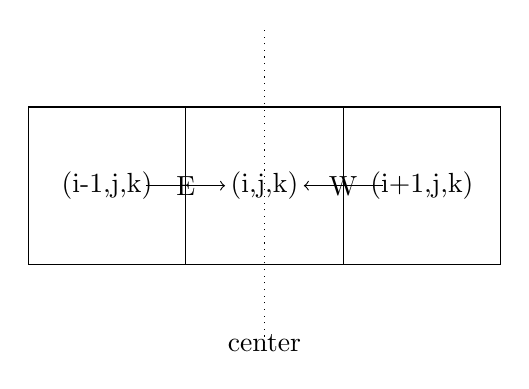
\begin{tikzpicture}
\draw (0,0) rectangle(2,2);
\draw (-2,0) rectangle(2,2);
\draw [->] (-2.5,1) -- (-1.5,1) node(g) at (-2,1) {E};
\draw (1,1) node(a) {(i+1,j,k)};
\draw (-1,1) node(b) {(i,j,k)};
\draw (-3,1) node(c) {(i-1,j,k)};
\draw [dotted](-1,-1) -- (-1,3) node (f) at (-1,-1) {center};
\draw [->] (0.5,1) -- (-0.5,1) node(h) at (0,1) {W};
\draw (-4,0) rectangle(2,2);
\end{tikzpicture}
\caption{streamwise direction}
\end{figure}

\begin{align}
\begin{split}
& u_{i,j,k}^{n+\frac{1}{2},E} = u_{i-\frac{1}{2},j,k}^n + \frac{\Delta x}{2}\frac{\partial u}{\partial x}|_{i-\frac{1}{2},j,k} + \frac{\Delta t}{2}\frac{\partial u}{\partial t}|_{i-\frac{1}{2},j,k}\\
&= u_{i-\frac{1}{2},j,k}^n + \frac{\Delta x}{2} \frac{\partial u}{\partial x} + \frac{\Delta t}{2} \Big( -u\frac{\partial u}{\partial x} -v\frac{\partial u}{\partial y} -w\frac{\partial u}{\partial z} - \frac{1}{\rho}\frac{\partial p}{\partial x} +\frac{1}{\rho}\tau_X\Big) \\
&= \underbrace{u_{i-\frac{1}{2},j,k}^n + \Big(\frac{\Delta x}{2} - \frac{\Delta t}{2} u_{i-\frac{1}{2},j,k}^n\Big)\frac{\partial u}{\partial x}|_{i-\frac{1}{2},j,k}}_\text{$\widehat{u}_{i,j,k}^{n+\frac{1}{2},E}$ normal term} -\underbrace{\frac{\Delta t}{2}v\frac{\partial u}{\partial y} - \frac{\Delta t}{2}w\frac{\partial u}{\partial z}}_\text{transverse term} - \frac{\Delta t}{2}\frac{1}{\rho}\frac{\partial p}{\partial x} + \frac{\Delta t}{2}\frac{1}{\rho}\tau_X \\
\end{split}
\end{align}

\begin{align}
\begin{split}
& u_{i,j,k}^{n+\frac{1}{2},W} = u_{i+\frac{1}{2},j,k}^n - \frac{\Delta x}{2}\frac{\partial u}{\partial x}|_{i+\frac{1}{2},j,k} + \frac{\Delta t}{2}\frac{\partial u}{\partial t}|_{i+\frac{1}{2},j,k}\\
&= u_{i+\frac{1}{2},j,k}^n - \frac{\Delta x}{2} \frac{\partial u}{\partial x} + \frac{\Delta t}{2} \Big( -u\frac{\partial u}{\partial x} -v\frac{\partial u}{\partial y} -w\frac{\partial u}{\partial z} - \frac{1}{\rho}\frac{\partial p}{\partial x} + \frac{1}{\rho}\tau_X\Big) \\
&= \underbrace{u_{i+\frac{1}{2},j,k}^n + \Big(-\frac{\Delta x}{2} - \frac{\Delta t}{2} u_{i+\frac{1}{2},j,k}^n\Big)\frac{\partial u}{\partial x}}_\text{$\widehat{u}_{i,j,k}^{n+\frac{1}{2},W}$ normal term} -\underbrace{\frac{\Delta t}{2}v\frac{\partial u}{\partial y} - \frac{\Delta t}{2}w\frac{\partial u}{\partial z}}_\text{transverse term} - \frac{\Delta t}{2}\frac{1}{\rho}\frac{\partial p}{\partial x} + \frac{\Delta t}{2}\frac{1}{\rho}\tau_X \\
\end{split}
\end{align}


\begin{figure}[!htb]
\centering
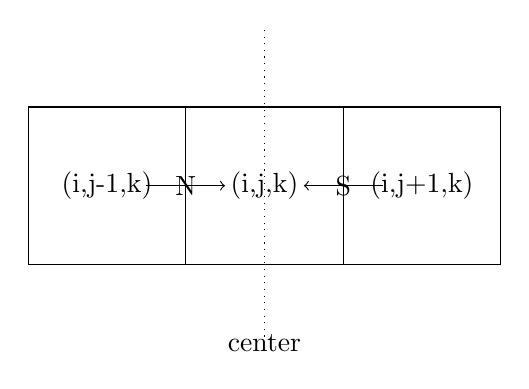
\begin{tikzpicture}
\draw (0,0) rectangle(2,2);
\draw (-2,0) rectangle(2,2);
\draw [->] (-2.5,1) -- (-1.5,1) node(g) at (-2,1) {N};
\draw (1,1) node(a) {(i,j+1,k)};
\draw (-1,1) node(b) {(i,j,k)};
\draw (-3,1) node(c) {(i,j-1,k)};
\draw [dotted](-1,-1) -- (-1,3) node (f) at (-1,-1) {center};
\draw [->] (0.5,1) -- (-0.5,1) node(h) at (0,1) {S};
\draw (-4,0) rectangle(2,2);
\end{tikzpicture}
\caption{spanwise direction}
\end{figure}

\begin{align}
\begin{split}
& v_{i,j,k}^{n+\frac{1}{2},N} = v_{i,j-\frac{1}{2},k}^n + \frac{\Delta y}{2}\frac{\partial v}{\partial y}|_{i,j-\frac{1}{2},k} + \frac{\Delta t}{2}\frac{\partial v}{\partial t}|_{i,j-\frac{1}{2},k}\\
&= v_{i,j-\frac{1}{2},k}^n + \frac{\Delta y}{2} \frac{\partial v}{\partial y}|_{i,j-\frac{1}{2},k} + \frac{\Delta t}{2} \Big( -u\frac{\partial v}{\partial x} -v\frac{\partial v}{\partial y} -w\frac{\partial v}{\partial z} - \frac{1}{\rho}\frac{\partial p}{\partial y} + \frac{1}{\rho}\tau_Y\Big) \\
&= \underbrace{v_{i,j-\frac{1}{2},k}^n + \Big(\frac{\Delta y}{2} - \frac{\Delta t}{2} v_{i,j-\frac{1}{2},k}^n\Big)\frac{\partial v}{\partial y}|_{i,j-\frac{1}{2},k}}_\text{$\widehat{v}_{i,j,k}^{n+\frac{1}{2},N}$ normal term} -\underbrace{\frac{\Delta t}{2}u\frac{\partial v}{\partial x} - \frac{\Delta t}{2}w\frac{\partial v}{\partial z}}_\text{transverse term} - \frac{\Delta t}{2}\frac{1}{\rho}\frac{\partial p}{\partial y} + \frac{\Delta t}{2}\frac{1}{\rho}\tau_Y \\
\end{split}
\end{align}

\begin{align}
\begin{split}
& v_{i,j,k}^{n+\frac{1}{2},S} = v_{i,j+\frac{1}{2},k}^n - \frac{\Delta y}{2}\frac{\partial v}{\partial y}|_{i,j+\frac{1}{2},k} + \frac{\Delta t}{2}\frac{\partial v}{\partial t}|_{i,j+\frac{1}{2},k}\\
&= v_{i,j+\frac{1}{2},k}^n - \frac{\Delta y}{2} \frac{\partial v}{\partial y}|_{i,j+\frac{1}{2},k} + \frac{\Delta t}{2} \Big( -u\frac{\partial v}{\partial x} -v\frac{\partial v}{\partial y} -w\frac{\partial v}{\partial z} - \frac{1}{\rho}\frac{\partial p}{\partial y} + \frac{1}{\rho}\tau_Y\Big) \\
&= \underbrace{v_{i,j+\frac{1}{2},k}^n + \Big(-\frac{\Delta y}{2} - \frac{\Delta t}{2} v_{i,j+\frac{1}{2},k}^n\Big)\frac{\partial v}{\partial y}|_{i,j-\frac{1}{2},k}}_\text{$\widehat{v}_{i,j,k}^{n+\frac{1}{2},S}$ normal term} -\underbrace{\frac{\Delta t}{2}u\frac{\partial v}{\partial x} - \frac{\Delta t}{2}w\frac{\partial v}{\partial z}}_\text{transverse term} - \frac{\Delta t}{2}\frac{1}{\rho}\frac{\partial p}{\partial y} + \frac{\Delta t}{2}\frac{1}{\rho}\tau_Y \\
\end{split}
\end{align}

\begin{figure}[!htb]
\centering
\begin{tikzpicture}
\draw (0,0) rectangle(2,2);
\draw (0,-2) rectangle(2,2);
\draw [->] (1,-2.5) -- (1,-1.5) node(g) at (1,-2) {T};
\draw (1,1) node(a) {(i,j,k+1)};
\draw (1,-1) node(b) {(i,j,k)};
\draw (1,-3) node(c) {(i,j,k-1)};
\draw [dotted](-1,-1) -- (3,-1) node (f) at (-1,-1) {center};
\draw [->] (1,0.5) -- (1,-0.5) node(h) at (1,0) {B};
\draw (0,-4) rectangle(2,2);
\end{tikzpicture}
\caption{vertical direction}
\end{figure}


\begin{align}
\begin{split}
& w_{i,j,k}^{n+\frac{1}{2},T} = w_{i,j,k-\frac{1}{2}}^n + \frac{\Delta z}{2}\frac{\partial w}{\partial z}|_{i,j,k-\frac{1}{2}} + \frac{\Delta t}{2}\frac{\partial w}{\partial t}|_{i,j,k-\frac{1}{2}}\\
&= w_{i,j,k-\frac{1}{2}}^n + \frac{\Delta z}{2} \frac{\partial w}{\partial z}|_{i,j,k-\frac{1}{2}} + \frac{\Delta t}{2} \Big( -u\frac{\partial w}{\partial x} -v\frac{\partial w}{\partial y} -w\frac{\partial w}{\partial z} - \frac{1}{\rho}\frac{\partial p}{\partial z} + \frac{1}{\rho}\tau_Z + g\Big) \\
&= \underbrace{w_{i,j,k-\frac{1}{2}}^n + \Big(\frac{\Delta z}{2} - \frac{\Delta t}{2} w_{i,j,k-\frac{1}{2}}^n\Big)\frac{\partial w}{\partial z}|_{i,j,k-\frac{1}{2}}}_\text{$\widehat{w}_{i,j,k}^{n+\frac{1}{2},T}$ normal term} -\underbrace{\frac{\Delta t}{2}u\frac{\partial w}{\partial x} - \frac{\Delta t}{2}v\frac{\partial w}{\partial y}}_\text{transverse term} - \frac{\Delta t}{2}\frac{1}{\rho}\frac{\partial p}{\partial y} + \frac{\Delta t}{2}\frac{1}{\rho}\tau_Z + \Delta t \cdot g \\
\end{split}
\end{align}

\begin{align}
\begin{split}
& w_{i,j,k}^{n+\frac{1}{2},B} = w_{i,j,k+\frac{1}{2}}^n - \frac{\Delta z}{2}\frac{\partial w}{\partial z}|_{i,j,k+\frac{1}{2}} + \frac{\Delta t}{2}\frac{\partial w}{\partial t}|_{i,j,k+\frac{1}{2}}\\
&= w_{i,j,k-\frac{1}{2}}^n - \frac{\Delta z}{2} \frac{\partial w}{\partial z}|_{i,j,k-\frac{1}{2}} + \frac{\Delta t}{2} \Big( -u\frac{\partial w}{\partial x} -v\frac{\partial w}{\partial y} -w\frac{\partial w}{\partial z} - \frac{1}{\rho}\frac{\partial p}{\partial z} + \frac{1}{\rho}\tau_Z + g\Big) \\
&= \underbrace{w_{i,j,k+\frac{1}{2}}^n + \Big(-\frac{\Delta z}{2} - \frac{\Delta t}{2} w_{i,j,k+\frac{1}{2}}^n\Big)\frac{\partial w}{\partial z}|_{i,j,k+\frac{1}{2}}}_\text{$\widehat{w}_{i,j,k}^{n+\frac{1}{2},B}$ normal term} -\underbrace{\frac{\Delta t}{2}u\frac{\partial w}{\partial x} - \frac{\Delta t}{2}v\frac{\partial w}{\partial y}}_\text{transverse term} - \frac{\Delta t}{2}\frac{1}{\rho}\frac{\partial p}{\partial y} + \frac{\Delta t}{2}\frac{1}{\rho}\tau_Z+ \Delta t \cdot g \\
\end{split}
\end{align}



%----------------------------------------------------------------------------------------
%	SECTION Normal Velocities on Cell Centers
%----------------------------------------------------------------------------------------
\subsubsection{Normal velocities on cell centers}
\begin{equation}
    \widehat{u}_{i,j,k}^{n+\frac{1}{2}, W},
\widehat{u}_{i,j,k}^{n+\frac{1}{2}, E},
\widehat{v}_{i,j,k}^{n+\frac{1}{2}, N},
\widehat{v}_{i,j,k}^{n+\frac{1}{2}, S},
\widehat{w}_{i,j,k}^{n+\frac{1}{2}, B},
\widehat{w}_{i,j,k}^{n+\frac{1}{2}, T}
\end{equation}

Take Direction EAST for example,
\begin{equation}
\widehat{u}_{i,j,k}^{n+\frac{1}{2},E} =
\underbrace{{u_{i-\frac{1}{2},j,k}^n}}_\text{$u^n$} + \Big(\frac{\Delta x}{2} - \frac{\Delta t}{2} u_{i-\frac{1}{2},j,k}^n\Big) \underbrace{\frac{\partial u}{\partial x}}_\text{slope limiter} |_{i-\frac{1}{2},j,k}
\end{equation}


%%%%%%% Figure about Boundary Condition will go to an individual chapter.
\begin{comment}
\begin{figure}[!htb]
\centering
\begin{tikzpicture}
\draw (0,0) rectangle(2,2);
\draw (1,1) node(qs) {5};
\draw (-1,1) node(qasb) {state U2};
\draw (0,-2) rectangle(2,2);
\draw (1,-1) node(qb) {index};
\draw (-1,-1) node(hjg) {state U1};
\draw (0,-4) rectangle(2,2);
\draw (1,-3) node(qc) {4};
\draw (-1,-3) node(adlo) {state U0};
\draw [->] (1.5,-1) -- (2.5,-1) node(qds) at(2,-1) {u};
\draw [dotted] [->] (1.5,-3) -- (2.5,-3) node(qdsfs) at(2,-3) {u=0};
\draw (-3,-2) -- (5,-2) node(ac) at (4,-2) [below]{Lower Neumann B.C.};
\end{tikzpicture}
\caption{stencil in EAST direction Z axis}
\end{figure}
\end{comment}



For slope limiter, we apply a first-order monotonicity slope limiter to the normal derivatives.[09.a second-order projection method for the incompressible navier-stokes equations.pdf] \\
For U-Face, calculate $u_x$, $u_y$, $u_z$ :\\
For V-Face, calculate $v_x$, $v_y$, $v_z$ : \\
For W-Face, calculate $w_x$, $w_y$, $w_z$ : \\


%%%%% Details caclulation will replace here.
\begin{comment}
for $X,Y$ axises, no special treatment due to Periodic Boundary Condition.\\
for $Z$ axis at lower boundary from EAST,
\begin{align}
\begin{split}
    \overline{(\Delta u)}^{(x)}_{i-\frac{1}{2},j,k} &= EBMminmod(\frac{U1.u-0.0}{\frac{dz}{2}}, \frac{U2.u-U1.u}{dz})\\
          &= EBMminmod(\frac{2.0*U1.u}{dz}, \frac{U2.u-U1.u}{dz}) 
\end{split}
\end{align}

for Z axis at upper boundary, it follows the same fashion.
For V-Face, calculating $v_x$, $v_y$, $v_z$, it has the same pattern as calculating U-Face.
For W-Face, calculating $w_z$ at lower boundary
\begin{align}
\begin{split}
    \overline{(\Delta w)}^{(z)}_{i-\frac{1}{2},j,k} &= EBMminmod(\frac{U1.u-0.0}{\frac{dz}{2}}, \frac{U2.u-U1.u}{dz})\\
          &= EBMminmod(\frac{2.0*U1.u}{dz}, \frac{U2.u-U1.u}{dz}) 
\end{split}
\end{align}


When calculating $w-z$ at upper boundary:
\begin{align}
\begin{split}
    \overline{(\Delta w)}^{(z)}_{i-\frac{1}{2},j,k}  &= EBMminmod(\frac{0.0 - U0.u}{dz}, \frac{-U0.u-0.0}{dz}) 
\end{split}
\end{align}
\end{comment}




%----------------------------------------------------------------------------------------
%	SECTION Update Transverse Velocities
%----------------------------------------------------------------------------------------
\subsubsection{Update transverse velocities and more}
Transverse terms on \framebox{U-Face} are
\begin{equation}
    v\frac{\partial u}{\partial y} + w\frac{\partial u}{\partial z}
\end{equation}

we need information for $v$ and $w$ at $(i-\frac{1}{2},j,k)$.\\
Approximate $v_{i-\frac{1}{2},j,k}$ as:
\begin{equation}
v_{i-\frac{1}{2},j,k} =
	\begin{cases}
	= \frac{1}{2}v_{i-\frac{1}{2},j+\frac{1}{2},k}
		\begin{cases}
		\frac{1}{2}v_{i-1,j+\frac{1}{2},k} \\
		\frac{1}{2}v_{i,j+\frac{1}{2},k} \\
		\end{cases}\\
	= \frac{1}{2}v_{i-\frac{1}{2},j-\frac{1}{2},k}
		\begin{cases}
		\frac{1}{2}v_{i-1,j-\frac{1}{2},k} \\
		\frac{1}{2}v_{i,j-\frac{1}{2},k}\\
		\end{cases}\\
	\end{cases}
\end{equation}

and,
\begin{equation}
    \frac{\Delta t}{2}v\frac{\partial u}{\partial y} - \frac{\Delta t}{2}w\frac{\partial u}{\partial z}|_{i-\frac{1}{2},j,k}
\end{equation}
Approximate $\frac{\partial u}{\partial y}$ as:
\begin{equation}
    \frac{\partial u}{\partial y}|_{i-\frac{1}{2},j,k}= 
\end{equation}

on \framebox{V-Face} are
\begin{equation}
    u\frac{\partial v}{\partial x} + w\frac{\partial v}{\partial z}
\end{equation}
on \framebox{W-Faces}are
\begin{equation}
    u\frac{\partial w}{\partial x} + v\frac{\partial w}{\partial y}
\end{equation}



%----------------------------------------------------------------------------------------
%	SECTION Riemann Solver in Upwinding fashion
%----------------------------------------------------------------------------------------
\subsubsection{Upwind scheme}
A Riemann solver will be employed to uniquely determine cell center velocities in an upwind fashion.
\begin{equation}
u_{i,j,k}^{n+\frac{1}{2}} = \verb|Riemann_Solver| \Big( u_{i,j,k}^{n+\frac{1}{2},E}, u_{i,j,k}^{n+\frac{1}{2},W} \Big)
\end{equation}
\begin{equation}
v_{i,j,k}^{n+\frac{1}{2}} = \verb|Riemann_Solver| \Big( v_{i,j,k}^{n+\frac{1}{2},N}, v_{i,j,k}^{n+\frac{1}{2},S} \Big)
\end{equation}
\begin{equation}
w_{i,j,k}^{n+\frac{1}{2}} = \verb|Riemann_Solver| \Big( w_{i,j,k}^{n+\frac{1}{2},T}, w_{i,j,k}^{n+\frac{1}{2},B} \Big)
\end{equation}


%----------------------------------------------------------------------------------------
%	SECTION Cell Face Velocity advected at half time step
%----------------------------------------------------------------------------------------
\subsection{Cell Face Velocity advected at half time step}
\begin{align}
\begin{split}
& u_{i+\frac{1}{2},j,k}^{n+\frac{1}{2}} = u_{i+\frac{1}{2},j,k}^n + \frac{\Delta t}{2}\frac{\partial u}{\partial t}|_{i+\frac{1}{2},j,k}\\
& = u_{i+\frac{1}{2},j,k}^n + \frac{\Delta t}{2} \Big( -u\frac{\partial u}{\partial x} -v\frac{\partial u}{\partial y} -w\frac{\partial u}{\partial z} - \frac{1}{\rho}\frac{\partial p}{\partial x} + \frac{1}{\rho}\tau_X\Big) \\
& = \underbrace{u_{i+\frac{1}{2},j,k}^n + \Big( - \frac{\Delta t}{2} u_{i+\frac{1}{2},j,k}^n\Big)\frac{\partial u}{\partial x}|_{i+\frac{1}{2},j,k}}_\text{$\widehat{u}_{i+\frac{1}{2},j,k}^{n+\frac{1}{2}}$ normal term} -\underbrace{\frac{\Delta t}{2}v\frac{\partial u}{\partial y} - \frac{\Delta t}{2}w\frac{\partial u}{\partial z}}_\text{transverse term} - \frac{\Delta t}{2}\frac{1}{\rho}\frac{\partial p}{\partial x} + \frac{\Delta t}{2}\frac{1}{\rho}\tau_X \\
\end{split}
\end{align}

\begin{align}
\begin{split}
& v_{i,j+\frac{1}{2},k}^{n+\frac{1}{2}} = v_{i,j+\frac{1}{2},k}^n + \frac{\Delta t}{2}\frac{\partial v}{\partial t}|_{i,j+\frac{1}{2},k}\\
& = v_{i,j+\frac{1}{2},k}^n + \frac{\Delta t}{2} \Big( -u\frac{\partial v}{\partial x} -v\frac{\partial v}{\partial y} -w\frac{\partial v}{\partial z} - \frac{1}{\rho}\frac{\partial p}{\partial y} + \frac{1}{\rho}\tau_Y\Big) \\
& = \underbrace{v_{i,j+\frac{1}{2},k}^n + \Big( - \frac{\Delta t}{2} v_{i,j+\frac{1}{2},k}^n\Big)\frac{\partial v}{\partial y}|_{i,j+\frac{1}{2},k}}_\text{$\widehat{v}_{i,j+\frac{1}{2},k}^{n+\frac{1}{2}}$ normal term} -\underbrace{\frac{\Delta t}{2}u\frac{\partial v}{\partial x} - \frac{\Delta t}{2}w\frac{\partial v}{\partial z}}_\text{transverse term} - \frac{\Delta t}{2}\frac{1}{\rho}\frac{\partial p}{\partial y} + \frac{\Delta t}{2}\frac{1}{\rho}\tau_Y \\
\end{split}
\end{align}

\begin{align}
\begin{split}
& w_{i,j,k+\frac{1}{2}}^{n+\frac{1}{2}} = w_{i,j,k+\frac{1}{2}}^n + \frac{\Delta t}{2}\frac{\partial w}{\partial t}|_{i,j,k+\frac{1}{2}}\\
& = w_{i,j,k+\frac{1}{2}}^n + \frac{\Delta t}{2} \Big( -u\frac{\partial w}{\partial x} -v\frac{\partial w}{\partial y} -w\frac{\partial w}{\partial z} - \frac{1}{\rho}\frac{\partial p}{\partial z} + \frac{1}{\rho}\tau_Y + g\Big) \\
& = \underbrace{w_{i,j,k+\frac{1}{2}}^n + \Big( - \frac{\Delta t}{2} w_{i,j,k+\frac{1}{2}}^n\Big)\frac{\partial w}{\partial z}|_{i,j,k+\frac{1}{2}}}_\text{$\widehat{w}_{i,j,k+\frac{1}{2}}^{n+\frac{1}{2}}$ normal term} -\underbrace{\frac{\Delta t}{2}u\frac{\partial w}{\partial x} - \frac{\Delta t}{2}v\frac{\partial w}{\partial y}}_\text{transverse term} - \frac{\Delta t}{2}\frac{1}{\rho}\frac{\partial p}{\partial z} + \frac{\Delta t}{2}\frac{1}{\rho}\tau_Z + \Delta t \cdot g \\
\end{split}
\end{align}



%----------------------------------------------------------------------------------------
%	SECTION MAC-Type Projection - First Poisson Equation for PETSc
%----------------------------------------------------------------------------------------
\subsubsection{MAC-Type Projection - First Poisson Equation for PETSc}
Extrapolate in only time to obtain cell-face velocities $u^{n+\frac{1}{2}}_{i+\frac{1}{2},j,k}$, $v^{n+\frac{1}{2}}_{i,j+\frac{1}{2},k}$,$w^{n+\frac{1}{2}}_{i,j,k+\frac{1}{2}}$ on u-face, v-face and w-face, respectively. This was done in the above section. Now perform a MAC-type projection to enforce the divergence constraint on the face velocities.
\begin{equation}
    \bigtriangledown \cdot U = - \bigtriangledown \cdot \Big( \frac{D}{\rho}\bigtriangledown \rho\Big) := S
\end{equation}

Use the reference paper [47], we solve the following equation for $\Phi$:
\begin{equation}
\Big( D \frac{1}{\rho ^n} G \Phi \Big)_{ijk} = D U^{n+\frac{1}{2}}_{ijk} -S^n_{ijk}
\end{equation}

where 
\begin{equation}
\Big(D \frac{1}{\rho^n} G \Phi \Big)_{ijk}
\end{equation}

can be discretized as a density-weighted compact 7 point stencil, $S$ is defined in the divergence constraint equation above. \\
To begin with, identify compact 7 point stencil:
\begin{equation}
\Phi_{i,j,k-1}, \Phi_{i,j-1,k}, \Phi_{i-1,j,k}, \Phi_{i,j,k}, \Phi_{i+1,j,k}, \Phi_{i,j+1,k}, \Phi_{i,j,k+1}
\end{equation}

so, expand LHS:
\begin{align}
\begin{split}
& D\frac{1}{\rho^n}G\Phi_{i,j,k} = \\
& \frac{1}{\Delta x}\Big(\frac{1}{\rho^n_{i+\frac{1}{2},j,k}}\frac{\Phi_{i+1,j,k} - \Phi_{i,j,k}}{\Delta x} - \frac{1}{\rho^n_{i-\frac{1}{2},j,k}}\frac{\Phi_{i,j,k} - \Phi_{i-1,j,k}}{\Delta x}\Big) \\
& + \frac{1}{\Delta y}\Big(\frac{1}{\rho^n_{i,j+\frac{1}{2},k}}\frac{\Phi_{i,j+1,k} - \Phi_{i,j,k}}{\Delta y} - \frac{1}{\rho^n_{i,j-\frac{1}{2},k}}\frac{\Phi_{i,j,k} - \Phi_{i,j-1,k}}{\Delta y}\Big) \\
& + \frac{1}{\Delta z}\Big(\frac{1}{\rho^n_{i,j,k+\frac{1}{2}}}\frac{\Phi_{i,j,k+1} - \Phi_{i,j,k}}{\Delta z} - \frac{1}{\rho^n_{i,j,k-\frac{1}{2}}}\frac{\Phi_{i,j,k} - \Phi_{i,j,k-1}}{\Delta z}\Big)
\end{split}
\end{align}

Calculate the right hand side $DU^{n+\frac{1}{2}}_{ijk}$ using cell-face velocities:
\begin{align}
\begin{split}
DU^{n+\frac{1}{2}}_{ijk} &= \frac{u^{n+\frac{1}{2}}_{i+\frac{1}{2},j,k} - u^{n+\frac{1}{2}}_{i-\frac{1}{2},j,k}}{\Delta x} + \frac{v^{n+\frac{1}{2}}_{i,j+\frac{1}{2},k} - v^{n+\frac{1}{2}}_{i,j-\frac{1}{2},k}}{\Delta y} + \frac{w^{n+\frac{1}{2}}_{i,j,k+\frac{1}{2}} - w^{n+\frac{1}{2}}_{i,j,k-\frac{1}{2}}}{\Delta z}
\end{split}
\end{align}

Calculate $S^n_{i,j,k}$ using cell face values.\\
Diffusion coefficients $D$ don't evolve in time, so suppress time step notation.\\
Densities $\rho$ are different, involving predictor-corrector step. For predictor step, use the states from old time step $n$. For corrector step, use $n+\frac{1}{2}$.\\
For density, use $\Box$ as time notation.
\begin{equation}
S^n_{i,j,k} = - \Bigg( \frac{\partial}{\partial x} \Big( \frac{D}{\rho}\frac{\partial \rho}{\partial x} \Big)
		      + \frac{\partial}{\partial y} \Big( \frac{D}{\rho}\frac{\partial \rho}{\partial y} \Big) 
		      + \frac{\partial}{\partial z} \Big( \frac{D}{\rho}\frac{\partial \rho}{\partial z} \Big) \Bigg)_{i,j,k}
\end{equation}


$x$-term:
\begin{align}
\begin{split}
& \frac{\partial}{\partial x} \Big( \frac{D}{\rho}\frac{\partial \rho}{\partial x} \Big)_{i,j,k} \\
&= \frac{ (\frac{D}{\rho}\frac{\partial \rho}{\partial x})_{i+\frac{1}{2},j,k} - (\frac{D}{\rho}\frac{\partial \rho}{\partial x})_{i-\frac{1}{2},j,k} }{\Delta x} \\
& = \frac{1}{\Delta x}\frac{D_{i+\frac{1}{2},j,k}}{\rho^{\Box}_{i+\frac{1}{2},j,k}}\cdot \frac{\rho^{\Box}_{i+1,j,k} - \rho^{\Box}_{i,j,k}}{\Delta x}
- \frac{1}{\Delta x}\frac{D_{i-\frac{1}{2},j,k}}{\rho^{\Box}_{i-\frac{1}{2},j,k}}\cdot \frac{\rho^{\Box}_{i,j,k} - \rho^{\Box}_{i-1,j,k}}{\Delta x}\\
\end{split}
\end{align}


$y$-term:
\begin{align}
\begin{split}
& \frac{\partial}{\partial y} \Big( \frac{D}{\rho}\frac{\partial \rho}{\partial y} \Big)_{i,j,k} \\
&= \frac{ (\frac{D}{\rho}\frac{\partial \rho}{\partial y})_{i,j+\frac{1}{2},k} - (\frac{D}{\rho}\frac{\partial \rho}{\partial y})_{i,j-\frac{1}{2},k} }{\Delta y} \\
& = \frac{1}{\Delta y}\frac{D_{i,j+\frac{1}{2},k}}{\rho^{\Box}_{i,j+\frac{1}{2},k}}\cdot \frac{\rho^{\Box}_{i,j+1,k} - \rho^{\Box}_{i,j,k}}{\Delta y}
- \frac{1}{\Delta y}\frac{D_{i,j-\frac{1}{2},k}}{\rho^{\Box}_{i,j-\frac{1}{2},k}}\cdot \frac{\rho^{\Box}_{i,j,k} - \rho^{\Box}_{i,j-1,k}}{\Delta y}\\
\end{split}
\end{align}


$z$-term:
\begin{align}
\begin{split}
& \frac{\partial}{\partial z} \Big( \frac{D}{\rho}\frac{\partial \rho}{\partial z} \Big)_{i,j,k} \\
&= \frac{ (\frac{D}{\rho}\frac{\partial \rho}{\partial z})_{i,j,k+\frac{1}{2}} - (\frac{D}{\rho}\frac{\partial \rho}{\partial z})_{i,j,k-\frac{1}{2}} }{\Delta z} \\
& = \frac{1}{\Delta z}\frac{D_{i,j,k+\frac{1}{2}}}{\rho^{\Box}_{i,j,k+\frac{1}{2}}}\cdot \frac{\rho^{\Box}_{i,j,k+1} - \rho^{\Box}_{i,j,k}}{\Delta z}
    - \frac{1}{\Delta z}\frac{D_{i,j,k-\frac{1}{2}}}{\rho^{\Box}_{i,j,k-\frac{1}{2}}}\cdot \frac{\rho^{\Box}_{i,j,k} - \rho^{\Box}_{i,j,k-1}}{\Delta z}\\
\end{split}
\end{align}

where $D$ and $\rho$ employed in the equations with $\frac{1}{2}$ indices are cell face values. Just average the two neighbor cell center values.\\
When all terms settled, solve the poisson equation with pure Neumann Boundary Condition. This is solved in PETSc.



%----------------------------------------------------------------------------------------
%	SECTION Form The first Coefficient Matrix
%----------------------------------------------------------------------------------------
\subsubsection{Form The First Coefficient Matrix}
\begin{equation}
A \Phi = b
\end{equation}
where $\Phi$s are the unknowns, $A$ is the coefficient matrix; $b$ is known.\\
The details will be given on a seperate chapter in the end.\\




%----------------------------------------------------------------------------------------
%	SECTION Update face velocities
%----------------------------------------------------------------------------------------
\subsubsection{Update face velocities}
New face velocities are:
\begin{equation}
u^{n+\frac{1}{2}}_{i+\frac{1}{2},j,k} \leftarrow u^{n+\frac{1}{2}}_{i+\frac{1}{2},j,k} - \frac{\Phi_{i+1,j,k} - \Phi_{i,j,k}}{\rho^n_{i+\frac{1}{2},j,k} \Delta x}
\end{equation}
\begin{equation}
v^{n+\frac{1}{2}}_{i,j+\frac{1}{2},k} \leftarrow v^{n+\frac{1}{2}}_{i,j+\frac{1}{2},k} - \frac{\Phi_{i,j+1,k} - \Phi_{i,j,k}}{\rho^n_{i,j+\frac{1}{2},k} \Delta y}
\end{equation}
\begin{equation}
w^{n+\frac{1}{2}}_{i,j,k+\frac{1}{2}} \leftarrow w^{n+\frac{1}{2}}_{i,j,k+\frac{1}{2}} - \frac{\Phi_{i,j,k+1} - \Phi_{i,j,k}}{\rho^n_{i,j,k+\frac{1}{2}} \Delta z}
\end{equation}
Notice: code is different. There is a $\Delta t$ term in source term, then cancelled out when calculating new cell face velocity.Check wenlin's thesis equation $(2.14-2.16)$. \\
Notice: $S^n$ is a lagged source term used in the projection, since $\rho^{n+\frac{1}{2}}$ is not available.



%----------------------------------------------------------------------------------------
%	SECTION Scalar on Boundary Condition
%----------------------------------------------------------------------------------------
\begin{comment}
\subsubsection{Treatment for Scalar on Boundary Condition}
For interior cells, just plug in numbers into the equations.\\
For boundary state, the corresponding state is a copy of the cell being looped over along the boundary state direction.\\
More discussion about boundary state will be detailed in Section 3.
\end{comment}


%----------------------------------------------------------------------------------------
%	SECTION Stencil used in MAC method
%----------------------------------------------------------------------------------------
\afterpage{% % defer placement until start of next page
%\subsection{Stencil used in MAC method}
\begin{figure}
\begin{center}
\includegraphics{pdfs/xyplane.pdf}
\caption{Stencil for MAC Grid X-Y plane}
\end{center}
\end{figure}


\begin{figure}
\begin{center}
\includegraphics{pdfs/yzplane.pdf}
\caption{Stencil for MAC Grid Y-Z plane}
\end{center}
\end{figure}


\begin{figure}
\begin{center}
\includegraphics{pdfs/xzplane.pdf}
\caption{Stencil for MAC Grid X-Z plane}
\end{center}
\end{figure}
\clearpage % if needed/desired
}% end of argument of \afterpage



%----------------------------------------------------------------------------------------
%	SECTION Cell-Edge Velocity at half time and half space
%----------------------------------------------------------------------------------------
\subsection{Cell-Edge Velocity at half time and half space}
Extrapolate in time and space to obtain cell-edge velocities.  
\begin{lstlisting}[frame=single]
u and v to vertical edges;
v and w to stream-wise edges;
u and w to span-wise edges.
\end{lstlisting}
An upwind-like scheme as Riemann solver will resolve the ambiguities. There is a 2-D version in reference [82]. The derivation of this section has the same precedure as calculating cell center velocities.\\

Neighbor Cell $I_{nb[7]}$:
\begin{align}
\begin{split}
& ul = u_{i+\frac{1}{2},j-\frac{1}{2},k}^{n+\frac{1}{2},N} = u_{i+\frac{1}{2},j-1,k}^n + \frac{\Delta y}{2}\frac{\partial u}{\partial y} + \frac{\Delta t}{2}\frac{\partial u}{\partial t}\\
&= u_{i+\frac{1}{2},j-1,k}^n + \frac{\Delta y}{2} \frac{\partial u}{\partial y} + \frac{\Delta t}{2} \Big( -u\frac{\partial u}{\partial x} -v\frac{\partial u}{\partial y} -w\frac{\partial u}{\partial z} - \frac{1}{\rho}\frac{\partial p}{\partial x} +\frac{1}{\rho}\tau_X\Big) \\
&= \underbrace{u_{i+\frac{1}{2},j-1,k}^n + \Big(\frac{\Delta y}{2}\frac{\partial u}{\partial y} - \frac{\Delta t}{2} u\frac{\partial u}{\partial x}\Big)}_\text{$\widehat{u}_{i+\frac{1}{2},j-\frac{1}{2},k}^{n+\frac{1}{2},N}$ normal term} -\underbrace{\frac{\Delta t}{2}v\frac{\partial u}{\partial y} - \frac{\Delta t}{2}w\frac{\partial u}{\partial z}}_\text{transverse term} - \frac{\Delta t}{2}\frac{1}{\rho}\frac{\partial p}{\partial x} + \frac{\Delta t}{2}\frac{1}{\rho}\tau_X
\end{split}
\end{align}

\begin{align}
\begin{split}
& ur = u_{i+\frac{1}{2},j-\frac{1}{2},k}^{n+\frac{1}{2},S} = u_{i+\frac{1}{2},j,k}^n - \frac{\Delta y}{2}\frac{\partial u}{\partial y} + \frac{\Delta t}{2}\frac{\partial u}{\partial t}\\
&= u_{i+\frac{1}{2},j,k}^n - \frac{\Delta y}{2} \frac{\partial u}{\partial y} + \frac{\Delta t}{2} \Big( -u\frac{\partial u}{\partial x} -v\frac{\partial u}{\partial y} -w\frac{\partial u}{\partial z} - \frac{1}{\rho}\frac{\partial p}{\partial x} +\frac{1}{\rho}\tau_X\Big) \\
&= \underbrace{u_{i+\frac{1}{2},j,k}^n + \Big(-\frac{\Delta y}{2}\frac{\partial u}{\partial y} - \frac{\Delta t}{2} u\frac{\partial u}{\partial x}\Big)}_\text{$\widehat{u}_{i+\frac{1}{2},j-\frac{1}{2},k}^{n+\frac{1}{2},S}$ normal term} -\underbrace{\frac{\Delta t}{2}v\frac{\partial u}{\partial y} - \frac{\Delta t}{2}w\frac{\partial u}{\partial z}}_\text{transverse term} - \frac{\Delta t}{2}\frac{1}{\rho}\frac{\partial p}{\partial x} + \frac{\Delta t}{2}\frac{1}{\rho}\tau_X
\end{split}
\end{align}

\begin{align}
\begin{split}
& vl = v_{i+\frac{1}{2},j-\frac{1}{2},k}^{n+\frac{1}{2},E} = v_{i,j-\frac{1}{2},k}^n + \frac{\Delta x}{2}\frac{\partial v}{\partial x} + \frac{\Delta t}{2}\frac{\partial v}{\partial t} \\
&= v_{i,j-\frac{1}{2},k}^n + \frac{\Delta x}{2} \frac{\partial v}{\partial x} + \frac{\Delta t}{2} \Big( -u\frac{\partial v}{\partial x} -v\frac{\partial v}{\partial y} -w\frac{\partial v}{\partial z} - \frac{1}{\rho}\frac{\partial p}{\partial y} +\frac{1}{\rho}\tau_Y\Big) \\
&= \underbrace{v_{i,j-\frac{1}{2},k}^n + \Big(\frac{\Delta x}{2}\frac{\partial v}{\partial x} - \frac{\Delta t}{2} v\frac{\partial v}{\partial y}\Big)}_\text{$\widehat{v}_{i+\frac{1}{2},j-\frac{1}{2},k}^{n+\frac{1}{2},E}$ normal term} -\underbrace{\frac{\Delta t}{2}u\frac{\partial v}{\partial x} - \frac{\Delta t}{2}w\frac{\partial v}{\partial z}}_\text{transverse term} - \frac{\Delta t}{2}\frac{1}{\rho}\frac{\partial p}{\partial y} + \frac{\Delta t}{2}\frac{1}{\rho}\tau_Y
\end{split}
\end{align}

\begin{align}
\begin{split}
& vr = v_{i+\frac{1}{2},j-\frac{1}{2},k}^{n+\frac{1}{2},W} = v_{i+1,j-\frac{1}{2},k}^n - \frac{\Delta x}{2}\frac{\partial v}{\partial x} + \frac{\Delta t}{2}\frac{\partial v}{\partial t} \\
&= v_{i+1,j-\frac{1}{2},k}^n - \frac{\Delta x}{2} \frac{\partial v}{\partial x} + \frac{\Delta t}{2} \Big( -u\frac{\partial v}{\partial x} -v\frac{\partial v}{\partial y} -w\frac{\partial v}{\partial z} - \frac{1}{\rho}\frac{\partial p}{\partial y} +\frac{1}{\rho}\tau_Y\Big) \\
&= \underbrace{v_{i+1,j-\frac{1}{2},k}^n + \Big(-\frac{\Delta x}{2}\frac{\partial v}{\partial x} - \frac{\Delta t}{2} v\frac{\partial v}{\partial y}\Big)}_\text{$\widehat{v}_{i+\frac{1}{2},j-\frac{1}{2},k}^{n+\frac{1}{2},W}$ normal term} -\underbrace{\frac{\Delta t}{2}u\frac{\partial v}{\partial x} - \frac{\Delta t}{2}w\frac{\partial v}{\partial z}}_\text{transverse term} - \frac{\Delta t}{2}\frac{1}{\rho}\frac{\partial p}{\partial y} + \frac{\Delta t}{2}\frac{1}{\rho}\tau_Y
\end{split}
\end{align}


Neighbor Cell $I_{nb[8]}$:
\begin{align}
\begin{split}
& ul = u_{i+\frac{1}{2},j+\frac{1}{2},k}^{n+\frac{1}{2},N} = u_{i+\frac{1}{2},j,k}^n + \frac{\Delta y}{2}\frac{\partial u}{\partial y} + \frac{\Delta t}{2}\frac{\partial u}{\partial t} \\
&= u_{i+\frac{1}{2},j,k}^n + \frac{\Delta y}{2} \frac{\partial u}{\partial y} + \frac{\Delta t}{2} \Big( -u\frac{\partial u}{\partial x} -v\frac{\partial u}{\partial y} -w\frac{\partial u}{\partial z} - \frac{1}{\rho}\frac{\partial p}{\partial x} +\frac{1}{\rho}\tau_X\Big) \\
&= \underbrace{u_{i+\frac{1}{2},j,k}^n + \Big(\frac{\Delta y}{2}\frac{\partial u}{\partial y} - \frac{\Delta t}{2} u\frac{\partial u}{\partial x}\Big)}_\text{$\widehat{u}_{i+\frac{1}{2},j+\frac{1}{2},k}^{n+\frac{1}{2},N}$ normal term} -\underbrace{\frac{\Delta t}{2}v\frac{\partial u}{\partial y} - \frac{\Delta t}{2}w\frac{\partial u}{\partial z}}_\text{transverse term} - \frac{\Delta t}{2}\frac{1}{\rho}\frac{\partial p}{\partial x} + \frac{\Delta t}{2}\frac{1}{\rho}\tau_X
\end{split}
\end{align}

\begin{align}
\begin{split}
& ur = u_{i+\frac{1}{2},j+\frac{1}{2},k}^{n+\frac{1}{2},S} = u_{i+\frac{1}{2},j+1,k}^n - \frac{\Delta y}{2}\frac{\partial u}{\partial y} + \frac{\Delta t}{2}\frac{\partial u}{\partial t} \\
&= u_{i+\frac{1}{2},j+1,k}^n - \frac{\Delta y}{2} \frac{\partial u}{\partial y} + \frac{\Delta t}{2} \Big( -u\frac{\partial u}{\partial x} -v\frac{\partial u}{\partial y} -w\frac{\partial u}{\partial z} - \frac{1}{\rho}\frac{\partial p}{\partial x} +\frac{1}{\rho}\tau_X\Big) \\
&= \underbrace{u_{i+\frac{1}{2},j+1,k}^n + \Big(-\frac{\Delta y}{2}\frac{\partial u}{\partial y} - \frac{\Delta t}{2} u\frac{\partial u}{\partial x}\Big)}_\text{$\widehat{u}_{i+\frac{1}{2},j+\frac{1}{2},k}^{n+\frac{1}{2},S}$ normal term} -\underbrace{\frac{\Delta t}{2}v\frac{\partial u}{\partial y} - \frac{\Delta t}{2}w\frac{\partial u}{\partial z}}_\text{transverse term} - \frac{\Delta t}{2}\frac{1}{\rho}\frac{\partial p}{\partial x} + \frac{\Delta t}{2}\frac{1}{\rho}\tau_X
\end{split}
\end{align}

\begin{align}
\begin{split}
& vl = v_{i+\frac{1}{2},j+\frac{1}{2},k}^{n+\frac{1}{2},E} = v_{i,j+\frac{1}{2},k}^n + \frac{\Delta x}{2}\frac{\partial v}{\partial x} + \frac{\Delta t}{2}\frac{\partial u}{\partial t} \\
&= v_{i,j+\frac{1}{2},k}^n + \frac{\Delta x}{2} \frac{\partial v}{\partial x} + \frac{\Delta t}{2} \Big( -u\frac{\partial v}{\partial x} -v\frac{\partial v}{\partial y} -w\frac{\partial v}{\partial z} - \frac{1}{\rho}\frac{\partial p}{\partial y} +\frac{1}{\rho}\tau_Y\Big) \\
&= \underbrace{v_{i,j+\frac{1}{2},k}^n + \Big(\frac{\Delta x}{2}\frac{\partial v}{\partial x} - \frac{\Delta t}{2} v\frac{\partial v}{\partial y}\Big)}_\text{$\widehat{v}_{i+\frac{1}{2},j+\frac{1}{2},k}^{n+\frac{1}{2},E}$ normal term} -\underbrace{\frac{\Delta t}{2}u\frac{\partial v}{\partial x} - \frac{\Delta t}{2}w\frac{\partial v}{\partial z}}_\text{transverse term} - \frac{\Delta t}{2}\frac{1}{\rho}\frac{\partial p}{\partial y} + \frac{\Delta t}{2}\frac{1}{\rho}\tau_Y
\end{split}
\end{align}

\begin{align}
\begin{split}
& vr = v_{i+\frac{1}{2},j+\frac{1}{2},k}^{n+\frac{1}{2},W} = v_{i+1,j+\frac{1}{2},k}^n - \frac{\Delta x}{2}\frac{\partial v}{\partial x} + \frac{\Delta t}{2}\frac{\partial u}{\partial t} \\
&= v_{i+1,j+\frac{1}{2},k}^n - \frac{\Delta x}{2} \frac{\partial v}{\partial x} + \frac{\Delta t}{2} \Big( -u\frac{\partial v}{\partial x} -v\frac{\partial v}{\partial y} -w\frac{\partial v}{\partial z} - \frac{1}{\rho}\frac{\partial p}{\partial y} +\frac{1}{\rho}\tau_Y\Big) \\
&= \underbrace{v_{i+1,j+\frac{1}{2},k}^n + \Big(-\frac{\Delta x}{2}\frac{\partial v}{\partial x} - \frac{\Delta t}{2} v\frac{\partial v}{\partial y}\Big)}_\text{$\widehat{v}_{i+\frac{1}{2},j+\frac{1}{2},k}^{n+\frac{1}{2},W}$ normal term} -\underbrace{\frac{\Delta t}{2}u\frac{\partial v}{\partial x} - \frac{\Delta t}{2}w\frac{\partial v}{\partial z}}_\text{transverse term} - \frac{\Delta t}{2}\frac{1}{\rho}\frac{\partial p}{\partial y} + \frac{\Delta t}{2}\frac{1}{\rho}\tau_Y
\end{split}
\end{align}

Neighbor Cell $I_{nb[9]}$:
\begin{align}
\begin{split}
& ul = u_{i-\frac{1}{2},j+\frac{1}{2},k}^{n+\frac{1}{2},N} = u_{i-\frac{1}{2},j,k}^n + \frac{\Delta y}{2}\frac{\partial u}{\partial y} + \frac{\Delta t}{2}\frac{\partial u}{\partial t} \\
&= u_{i-\frac{1}{2},j,k}^n + \frac{\Delta y}{2} \frac{\partial u}{\partial y} + \frac{\Delta t}{2} \Big( -u\frac{\partial u}{\partial x} -v\frac{\partial u}{\partial y} -w\frac{\partial u}{\partial z} - \frac{1}{\rho}\frac{\partial p}{\partial x} +\frac{1}{\rho}\tau_X\Big) \\
&= \underbrace{u_{i-\frac{1}{2},j,k}^n + \Big(\frac{\Delta y}{2}\frac{\partial u}{\partial y} - \frac{\Delta t}{2} u\frac{\partial u}{\partial x}\Big)}_\text{$\widehat{u}_{i-\frac{1}{2},j+\frac{1}{2},k}^{n+\frac{1}{2},N}$ normal term} -\underbrace{\frac{\Delta t}{2}v\frac{\partial u}{\partial y} - \frac{\Delta t}{2}w\frac{\partial u}{\partial z}}_\text{transverse term} - \frac{\Delta t}{2}\frac{1}{\rho}\frac{\partial p}{\partial x} + \frac{\Delta t}{2}\frac{1}{\rho}\tau_X
\end{split}
\end{align}

\begin{align}
\begin{split}
& ur = u_{i-\frac{1}{2},j+\frac{1}{2},k}^{n+\frac{1}{2},S} = u_{i-\frac{1}{2},j+1,k}^n - \frac{\Delta y}{2}\frac{\partial u}{\partial y} + \frac{\Delta t}{2}\frac{\partial u}{\partial t} \\
&= u_{i-\frac{1}{2},j+1,k}^n - \frac{\Delta y}{2} \frac{\partial u}{\partial y} + \frac{\Delta t}{2} \Big( -u\frac{\partial u}{\partial x} -v\frac{\partial u}{\partial y} -w\frac{\partial u}{\partial z} - \frac{1}{\rho}\frac{\partial p}{\partial x} +\frac{1}{\rho}\tau_X\Big) \\
&= \underbrace{u_{i-\frac{1}{2},j+1,k}^n + \Big(-\frac{\Delta y}{2}\frac{\partial u}{\partial y} - \frac{\Delta t}{2} u\frac{\partial u}{\partial x}\Big)}_\text{$\widehat{u}_{i-\frac{1}{2},j+\frac{1}{2},k}^{n+\frac{1}{2},S}$ normal term} -\underbrace{\frac{\Delta t}{2}v\frac{\partial u}{\partial y} - \frac{\Delta t}{2}w\frac{\partial u}{\partial z}}_\text{transverse term} - \frac{\Delta t}{2}\frac{1}{\rho}\frac{\partial p}{\partial x} + \frac{\Delta t}{2}\frac{1}{\rho}\tau_X
\end{split}
\end{align}

\begin{align}
\begin{split}
& vl = v_{i-\frac{1}{2},j+\frac{1}{2},k}^{n+\frac{1}{2},E} = v_{i-1,j+\frac{1}{2},k}^n + \frac{\Delta x}{2}\frac{\partial v}{\partial x} + \frac{\Delta t}{2}\frac{\partial u}{\partial t}\\
&= v_{i-1,j+\frac{1}{2},k}^n + \frac{\Delta x}{2} \frac{\partial v}{\partial x} + \frac{\Delta t}{2} \Big( -u\frac{\partial v}{\partial x} -v\frac{\partial v}{\partial y} -w\frac{\partial v}{\partial z} - \frac{1}{\rho}\frac{\partial p}{\partial y} +\frac{1}{\rho}\tau_Y\Big) \\
&= \underbrace{v_{i-1,j+\frac{1}{2},k}^n + \Big(\frac{\Delta x}{2}\frac{\partial v}{\partial x} - \frac{\Delta t}{2} v\frac{\partial v}{\partial y}\Big)}_\text{$\widehat{v}_{i-\frac{1}{2},j+\frac{1}{2},k}^{n+\frac{1}{2},E}$ normal term} -\underbrace{\frac{\Delta t}{2}u\frac{\partial v}{\partial x} - \frac{\Delta t}{2}w\frac{\partial v}{\partial z}}_\text{transverse term} - \frac{\Delta t}{2}\frac{1}{\rho}\frac{\partial p}{\partial y} + \frac{\Delta t}{2}\frac{1}{\rho}\tau_Y
\end{split}
\end{align}

\begin{align}
\begin{split}
& vr = v_{i-\frac{1}{2},j+\frac{1}{2},k}^{n+\frac{1}{2},W} = v_{i,j+\frac{1}{2},j,k}^n - \frac{\Delta x}{2}\frac{\partial v}{\partial x} + \frac{\Delta t}{2}\frac{\partial u}{\partial t}\\
&= v_{i,j+\frac{1}{2},k}^n - \frac{\Delta x}{2} \frac{\partial v}{\partial x} + \frac{\Delta t}{2} \Big( -u\frac{\partial v}{\partial x} -v\frac{\partial v}{\partial y} -w\frac{\partial v}{\partial z} - \frac{1}{\rho}\frac{\partial p}{\partial y} +\frac{1}{\rho}\tau_Y\Big) \\
&= \underbrace{v_{i,j+\frac{1}{2},k}^n + \Big(-\frac{\Delta x}{2}\frac{\partial v}{\partial x} - \frac{\Delta t}{2} v\frac{\partial v}{\partial y}\Big)}_\text{$\widehat{v}_{i-\frac{1}{2},j+\frac{1}{2},k}^{n+\frac{1}{2},W}$ normal term} -\underbrace{\frac{\Delta t}{2}u\frac{\partial v}{\partial x} - \frac{\Delta t}{2}w\frac{\partial v}{\partial z}}_\text{transverse term} - \frac{\Delta t}{2}\frac{1}{\rho}\frac{\partial p}{\partial y} + \frac{\Delta t}{2}\frac{1}{\rho}\tau_Y
\end{split}
\end{align}

Neighbor Cell $I_{nb[11]}$:
\begin{align}
\begin{split}
& vl = v_{i,j+\frac{1}{2},k-\frac{1}{2}}^{n+\frac{1}{2},T} = v_{i,j+\frac{1}{2},k-1}^n + \frac{\Delta z}{2}\frac{\partial v}{\partial z} + \frac{\Delta t}{2}\frac{\partial v}{\partial t} \\
&= v_{i,j+\frac{1}{2},k-1}^n + \frac{\Delta z}{2} \frac{\partial v}{\partial z} + \frac{\Delta t}{2} \Big( -u\frac{\partial v}{\partial x} -v\frac{\partial v}{\partial y} -w\frac{\partial v}{\partial z} - \frac{1}{\rho}\frac{\partial p}{\partial y} +\frac{1}{\rho}\tau_Y\Big) \\
&= \underbrace{v_{i,j+\frac{1}{2},k-1}^n + \Big(\frac{\Delta z}{2}\frac{\partial v}{\partial z} - \frac{\Delta t}{2} v\frac{\partial v}{\partial y}\Big)}_\text{$\widehat{v}_{i,j+\frac{1}{2},k-\frac{1}{2}}^{n+\frac{1}{2},T}$ normal term} -\underbrace{\frac{\Delta t}{2}u\frac{\partial v}{\partial x} - \frac{\Delta t}{2}w\frac{\partial v}{\partial z}}_\text{transverse term} - \frac{\Delta t}{2}\frac{1}{\rho}\frac{\partial p}{\partial y} + \frac{\Delta t}{2}\frac{1}{\rho}\tau_Y
\end{split}
\end{align}

\begin{align}
\begin{split}
& vr = v_{i,j+\frac{1}{2},k-\frac{1}{2}}^{n+\frac{1}{2},B} = v_{i,j+\frac{1}{2},k}^n - \frac{\Delta z}{2}\frac{\partial v}{\partial z} + \frac{\Delta t}{2}\frac{\partial v}{\partial t} \\
&= v_{i,j+\frac{1}{2},k}^n - \frac{\Delta z}{2} \frac{\partial v}{\partial z} + \frac{\Delta t}{2} \Big( -u\frac{\partial v}{\partial x} -v\frac{\partial v}{\partial y} -w\frac{\partial v}{\partial z} - \frac{1}{\rho}\frac{\partial p}{\partial y} +\frac{1}{\rho}\tau_Y\Big) \\
&= \underbrace{v_{i,j+\frac{1}{2},k}^n + \Big(-\frac{\Delta z}{2}\frac{\partial v}{\partial z} - \frac{\Delta t}{2} v\frac{\partial v}{\partial y}\Big)}_\text{$\widehat{v}_{i,j+\frac{1}{2},k-\frac{1}{2}}^{n+\frac{1}{2},B}$ normal term} -\underbrace{\frac{\Delta t}{2}u\frac{\partial v}{\partial x} - \frac{\Delta t}{2}w\frac{\partial v}{\partial z}}_\text{transverse term} - \frac{\Delta t}{2}\frac{1}{\rho}\frac{\partial p}{\partial y} + \frac{\Delta t}{2}\frac{1}{\rho}\tau_Y
\end{split}
\end{align}

\begin{align}
\begin{split}
& wl = w_{i,j+\frac{1}{2},k-\frac{1}{2}}^{n+\frac{1}{2},N} = w_{i,j,k-\frac{1}{2}}^n + \frac{\Delta y}{2}\frac{\partial w}{\partial y} + \frac{\Delta t}{2}\frac{\partial w}{\partial t} \\
&= w_{i,j,k-\frac{1}{2}}^n + \frac{\Delta y}{2} \frac{\partial w}{\partial y} + \frac{\Delta t}{2} \Big( -u\frac{\partial w}{\partial x} -v\frac{\partial w}{\partial y} -w\frac{\partial w}{\partial z} - \frac{1}{\rho}\frac{\partial p}{\partial z} +\frac{1}{\rho}\tau_Z + g\Big) \\
&= \underbrace{w_{i,j,k-\frac{1}{2}}^n + \Big(\frac{\Delta y}{2}\frac{\partial w}{\partial y} - \frac{\Delta t}{2} w\frac{\partial w}{\partial z}\Big)}_\text{$\widehat{w}_{i,j+\frac{1}{2},k-\frac{1}{2}}^{n+\frac{1}{2},N}$ normal term} -\underbrace{\frac{\Delta t}{2}u\frac{\partial w}{\partial x} - \frac{\Delta t}{2}v\frac{\partial w}{\partial y}}_\text{transverse term} - \frac{\Delta t}{2}\frac{1}{\rho}\frac{\partial p}{\partial z} + \frac{\Delta t}{2}\frac{1}{\rho}\tau_Z + \frac{\Delta t}{2}g
\end{split}
\end{align}

\begin{align}
\begin{split}
& wr = w_{i,j+\frac{1}{2},k-\frac{1}{2}}^{n+\frac{1}{2},S} = w_{i,j+1,k-\frac{1}{2}}^n - \frac{\Delta y}{2}\frac{\partial w}{\partial y} + \frac{\Delta t}{2}\frac{\partial v}{\partial t} \\
&= w_{i,j+1,k-\frac{1}{2}}^n - \frac{\Delta y}{2} \frac{\partial w}{\partial y} + \frac{\Delta t}{2} \Big( -u\frac{\partial w}{\partial x} -v\frac{\partial w}{\partial y} -w\frac{\partial w}{\partial z} - \frac{1}{\rho}\frac{\partial p}{\partial z} +\frac{1}{\rho}\tau_Z + g\Big) \\
&= \underbrace{w_{i,j+1,k-\frac{1}{2}}^n + \Big(-\frac{\Delta y}{2}\frac{\partial w}{\partial y} - \frac{\Delta t}{2} w\frac{\partial w}{\partial z}\Big)}_\text{$\widehat{w}_{i,j+\frac{1}{2},k-\frac{1}{2}}^{n+\frac{1}{2},S}$ normal term} -\underbrace{\frac{\Delta t}{2}u\frac{\partial w}{\partial x} - \frac{\Delta t}{2}v\frac{\partial w}{\partial y}}_\text{transverse term} - \frac{\Delta t}{2}\frac{1}{\rho}\frac{\partial p}{\partial z} + \frac{\Delta t}{2}\frac{1}{\rho}\tau_Z + \frac{\Delta t}{2}g
\end{split}
\end{align}

Neighbor Cell $I_{nb[12]}$:
\begin{align}
\begin{split}
& vl = v_{i,j+\frac{1}{2},k+\frac{1}{2}}^{n+\frac{1}{2},T} = v_{i,j+\frac{1}{2},k}^n + \frac{\Delta z}{2}\frac{\partial v}{\partial z} + \frac{\Delta t}{2}\frac{\partial v}{\partial t} \\
&= v_{i,j+\frac{1}{2},k}^n + \frac{\Delta z}{2} \frac{\partial v}{\partial z} + \frac{\Delta t}{2} \Big( -u\frac{\partial v}{\partial x} -v\frac{\partial v}{\partial y} -w\frac{\partial v}{\partial z} - \frac{1}{\rho}\frac{\partial p}{\partial y} +\frac{1}{\rho}\tau_Y\Big) \\
&= \underbrace{v_{i,j+\frac{1}{2},k}^n + \Big(\frac{\Delta z}{2}\frac{\partial v}{\partial z} - \frac{\Delta t}{2} v\frac{\partial v}{\partial y}\Big)}_\text{$\widehat{v}_{i,j+\frac{1}{2},k+\frac{1}{2}}^{n+\frac{1}{2},T}$ normal term} -\underbrace{\frac{\Delta t}{2}u\frac{\partial v}{\partial x} - \frac{\Delta t}{2}w\frac{\partial v}{\partial z}}_\text{transverse term} - \frac{\Delta t}{2}\frac{1}{\rho}\frac{\partial p}{\partial y} + \frac{\Delta t}{2}\frac{1}{\rho}\tau_Y
\end{split}
\end{align}

\begin{align}
\begin{split}
& vr = v_{i,j+\frac{1}{2},k+\frac{1}{2}}^{n+\frac{1}{2},B} = v_{i,j+\frac{1}{2},k+1}^n - \frac{\Delta z}{2}\frac{\partial v}{\partial z} + \frac{\Delta t}{2}\frac{\partial v}{\partial t} \\
&= v_{i,j+\frac{1}{2},k+1}^n - \frac{\Delta z}{2} \frac{\partial v}{\partial z} + \frac{\Delta t}{2} \Big( -u\frac{\partial v}{\partial x} -v\frac{\partial v}{\partial y} -w\frac{\partial v}{\partial z} - \frac{1}{\rho}\frac{\partial p}{\partial y} +\frac{1}{\rho}\tau_Y\Big) \\
&= \underbrace{v_{i,j+\frac{1}{2},k+1}^n + \Big(-\frac{\Delta z}{2}\frac{\partial v}{\partial z} - \frac{\Delta t}{2} v\frac{\partial v}{\partial y}\Big)}_\text{$\widehat{v}_{i,j+\frac{1}{2},k+\frac{1}{2}}^{n+\frac{1}{2},B}$ normal term} -\underbrace{\frac{\Delta t}{2}u\frac{\partial v}{\partial x} - \frac{\Delta t}{2}w\frac{\partial v}{\partial z}}_\text{transverse term} - \frac{\Delta t}{2}\frac{1}{\rho}\frac{\partial p}{\partial y} + \frac{\Delta t}{2}\frac{1}{\rho}\tau_Y
\end{split}
\end{align}

\begin{align}
\begin{split}
& wl = w_{i,j+\frac{1}{2},k+\frac{1}{2}}^{n+\frac{1}{2},N} = w_{i,j,k+\frac{1}{2}}^n + \frac{\Delta y}{2}\frac{\partial w}{\partial y} + \frac{\Delta t}{2}\frac{\partial v}{\partial t} \\
&= w_{i,j,k+\frac{1}{2}}^n + \frac{\Delta y}{2} \frac{\partial w}{\partial y} + \frac{\Delta t}{2} \Big( -u\frac{\partial w}{\partial x} -v\frac{\partial w}{\partial y} -w\frac{\partial w}{\partial z} - \frac{1}{\rho}\frac{\partial p}{\partial z} +\frac{1}{\rho}\tau_Z + g\Big) \\
&= \underbrace{w_{i,j,k+\frac{1}{2}}^n + \Big(\frac{\Delta y}{2}\frac{\partial w}{\partial y} - \frac{\Delta t}{2} w\frac{\partial w}{\partial z}\Big)}_\text{$\widehat{w}_{i,j+\frac{1}{2},k+\frac{1}{2}}^{n+\frac{1}{2},N}$ normal term} -\underbrace{\frac{\Delta t}{2}u\frac{\partial w}{\partial x} - \frac{\Delta t}{2}v\frac{\partial w}{\partial y}}_\text{transverse term} - \frac{\Delta t}{2}\frac{1}{\rho}\frac{\partial p}{\partial z} + \frac{\Delta t}{2}\frac{1}{\rho}\tau_Z + \frac{\Delta t}{2}g
\end{split}
\end{align}

\begin{align}
\begin{split}
& wr = w_{i,j+\frac{1}{2},k+\frac{1}{2}}^{n+\frac{1}{2},S} = w_{i,j+1,k+\frac{1}{2}}^n - \frac{\Delta y}{2}\frac{\partial w}{\partial y} + \frac{\Delta t}{2}\frac{\partial v}{\partial t} \\
&= w_{i,j+1,k+\frac{1}{2}}^n - \frac{\Delta y}{2} \frac{\partial w}{\partial y} + \frac{\Delta t}{2} \Big( -u\frac{\partial w}{\partial x} -v\frac{\partial w}{\partial y} -w\frac{\partial w}{\partial z} - \frac{1}{\rho}\frac{\partial p}{\partial z} +\frac{1}{\rho}\tau_Z + g\Big) \\
&= \underbrace{w_{i,j+1,k+\frac{1}{2}}^n + \Big(-\frac{\Delta y}{2}\frac{\partial w}{\partial y} - \frac{\Delta t}{2} w\frac{\partial w}{\partial z}\Big)}_\text{$\widehat{w}_{i,j+\frac{1}{2},k+\frac{1}{2}}^{n+\frac{1}{2},S}$ normal term} -\underbrace{\frac{\Delta t}{2}u\frac{\partial w}{\partial x} - \frac{\Delta t}{2}v\frac{\partial w}{\partial y}}_\text{transverse term} - \frac{\Delta t}{2}\frac{1}{\rho}\frac{\partial p}{\partial z} + \frac{\Delta t}{2}\frac{1}{\rho}\tau_Z + \frac{\Delta t}{2}g
\end{split}
\end{align}


Neighbor Cell $I_{nb[13]}$:
\begin{align}
\begin{split}
& vl = v_{i,j-\frac{1}{2},k+\frac{1}{2}}^{n+\frac{1}{2},T} = v_{i,j-\frac{1}{2},k}^n + \frac{\Delta z}{2}\frac{\partial v}{\partial z} + \frac{\Delta t}{2}\frac{\partial v}{\partial t} \\
&= v_{i,j-\frac{1}{2},k}^n + \frac{\Delta z}{2} \frac{\partial v}{\partial z} + \frac{\Delta t}{2} \Big( -u\frac{\partial v}{\partial x} -v\frac{\partial v}{\partial y} -w\frac{\partial v}{\partial z} - \frac{1}{\rho}\frac{\partial p}{\partial y} +\frac{1}{\rho}\tau_Y\Big) \\
&= \underbrace{v_{i,j-\frac{1}{2},k}^n + \Big(\frac{\Delta z}{2}\frac{\partial v}{\partial z} - \frac{\Delta t}{2} v\frac{\partial v}{\partial y}\Big)}_\text{$\widehat{v}_{i,j-\frac{1}{2},k+\frac{1}{2}}^{n+\frac{1}{2},T}$ normal term} -\underbrace{\frac{\Delta t}{2}u\frac{\partial v}{\partial x} - \frac{\Delta t}{2}w\frac{\partial v}{\partial z}}_\text{transverse term} - \frac{\Delta t}{2}\frac{1}{\rho}\frac{\partial p}{\partial y} + \frac{\Delta t}{2}\frac{1}{\rho}\tau_Y
\end{split}
\end{align}

\begin{align}
\begin{split}
& vr = v_{i,j-\frac{1}{2},k+\frac{1}{2}}^{n+\frac{1}{2},B} = v_{i,j-\frac{1}{2},k+1}^n - \frac{\Delta z}{2}\frac{\partial v}{\partial z} + \frac{\Delta t}{2}\frac{\partial v}{\partial t} \\
&= v_{i,j-\frac{1}{2},k+1}^n - \frac{\Delta z}{2} \frac{\partial v}{\partial z} + \frac{\Delta t}{2} \Big( -u\frac{\partial v}{\partial x} -v\frac{\partial v}{\partial y} -w\frac{\partial v}{\partial z} - \frac{1}{\rho}\frac{\partial p}{\partial y} +\frac{1}{\rho}\tau_Y\Big) \\
&= \underbrace{v_{i,j-\frac{1}{2},k+1}^n + \Big(-\frac{\Delta z}{2}\frac{\partial v}{\partial z} - \frac{\Delta t}{2} v\frac{\partial v}{\partial y}\Big)}_\text{$\widehat{v}_{i,j-\frac{1}{2},k+\frac{1}{2}}^{n+\frac{1}{2},B}$ normal term} -\underbrace{\frac{\Delta t}{2}u\frac{\partial v}{\partial x} - \frac{\Delta t}{2}w\frac{\partial v}{\partial z}}_\text{transverse term} - \frac{\Delta t}{2}\frac{1}{\rho}\frac{\partial p}{\partial y} + \frac{\Delta t}{2}\frac{1}{\rho}\tau_Y
\end{split}
\end{align}

\begin{align}
\begin{split}
& wl = w_{i,j-\frac{1}{2},k+\frac{1}{2}}^{n+\frac{1}{2},N} = w_{i,j-1,k+\frac{1}{2}}^n + \frac{\Delta y}{2}\frac{\partial w}{\partial y} + \frac{\Delta t}{2}\frac{\partial v}{\partial t} \\
&= w_{i,j-1,k+\frac{1}{2}}^n + \frac{\Delta y}{2} \frac{\partial w}{\partial y} + \frac{\Delta t}{2} \Big( -u\frac{\partial w}{\partial x} -v\frac{\partial w}{\partial y} -w\frac{\partial w}{\partial z} - \frac{1}{\rho}\frac{\partial p}{\partial z} +\frac{1}{\rho}\tau_Z + g\Big) \\
&= \underbrace{w_{i,j-1,k+\frac{1}{2}}^n + \Big(\frac{\Delta y}{2}\frac{\partial w}{\partial y} - \frac{\Delta t}{2} w\frac{\partial w}{\partial z}\Big)}_\text{$\widehat{w}_{i,j-\frac{1}{2},k+\frac{1}{2}}^{n+\frac{1}{2},N}$ normal term} -\underbrace{\frac{\Delta t}{2}u\frac{\partial w}{\partial x} - \frac{\Delta t}{2}v\frac{\partial w}{\partial y}}_\text{transverse term} - \frac{\Delta t}{2}\frac{1}{\rho}\frac{\partial p}{\partial z} + \frac{\Delta t}{2}\frac{1}{\rho}\tau_Z + \frac{\Delta t}{2}g
\end{split}
\end{align}

\begin{align}
\begin{split}
& wr = w_{i,j-\frac{1}{2},k+\frac{1}{2}}^{n+\frac{1}{2},S} = w_{i,j,k+\frac{1}{2}}^n + \frac{\Delta y}{2}\frac{\partial w}{\partial y} + \frac{\Delta t}{2}\frac{\partial v}{\partial t} \\
&= w_{i,j,k+\frac{1}{2}}^n - \frac{\Delta y}{2} \frac{\partial w}{\partial y} + \frac{\Delta t}{2} \Big( -u\frac{\partial w}{\partial x} -v\frac{\partial w}{\partial y} -w\frac{\partial w}{\partial z} - \frac{1}{\rho}\frac{\partial p}{\partial z} +\frac{1}{\rho}\tau_Z + g\Big) \\
&= \underbrace{w_{i,j,k+\frac{1}{2}}^n + \Big(-\frac{\Delta y}{2}\frac{\partial w}{\partial y} - \frac{\Delta t}{2} w\frac{\partial w}{\partial z}\Big)}_\text{$\widehat{w}_{i,j-\frac{1}{2},k+\frac{1}{2}}^{n+\frac{1}{2},S}$ normal term} -\underbrace{\frac{\Delta t}{2}u\frac{\partial w}{\partial x} - \frac{\Delta t}{2}v\frac{\partial w}{\partial y}}_\text{transverse term} - \frac{\Delta t}{2}\frac{1}{\rho}\frac{\partial p}{\partial z} + \frac{\Delta t}{2}\frac{1}{\rho}\tau_Z + \frac{\Delta t}{2}g
\end{split}
\end{align}


Neighbor Cell $I_{nb[15]}$:
\begin{align}
\begin{split}
& wl = w_{i+\frac{1}{2},j,k-\frac{1}{2}}^{n+\frac{1}{2},E} = w_{i,j,k-\frac{1}{2}}^n + \frac{\Delta x}{2}\frac{\partial w}{\partial x} + \frac{\Delta t}{2}\frac{\partial w}{\partial t} \\
&= w_{i,j,k-\frac{1}{2}}^n + \frac{\Delta x}{2} \frac{\partial w}{\partial x} + \frac{\Delta t}{2} \Big( -u\frac{\partial w}{\partial x} -v\frac{\partial w}{\partial y} -w\frac{\partial w}{\partial z} - \frac{1}{\rho}\frac{\partial p}{\partial z} +\frac{1}{\rho}\tau_Z + g\Big) \\
&= \underbrace{w_{i,j,k-\frac{1}{2}}^n + \Big(\frac{\Delta x}{2}\frac{\partial w}{\partial x} - \frac{\Delta t}{2} w\frac{\partial w}{\partial z}\Big)}_\text{$\widehat{w}_{i+\frac{1}{2},j,k-\frac{1}{2}}^{n+\frac{1}{2},E}$ normal term} -\underbrace{\frac{\Delta t}{2}u\frac{\partial w}{\partial x} - \frac{\Delta t}{2}v\frac{\partial w}{\partial y}}_\text{transverse term} - \frac{\Delta t}{2}\frac{1}{\rho}\frac{\partial p}{\partial z} + \frac{\Delta t}{2}\frac{1}{\rho}\tau_Z + \frac{\Delta t}{2}g
\end{split}
\end{align}

\begin{align}
\begin{split}
& wr = w_{i+\frac{1}{2},j,k-\frac{1}{2}}^{n+\frac{1}{2},W} = w_{i+1,j,k-\frac{1}{2}}^n - \frac{\Delta x}{2}\frac{\partial w}{\partial x} + \frac{\Delta t}{2}\frac{\partial w}{\partial t} \\
&= w_{i+1,j,k-\frac{1}{2}}^n - \frac{\Delta x}{2} \frac{\partial w}{\partial x} + \frac{\Delta t}{2} \Big( -u\frac{\partial w}{\partial x} -v\frac{\partial w}{\partial y} -w\frac{\partial w}{\partial z} - \frac{1}{\rho}\frac{\partial p}{\partial z} +\frac{1}{\rho}\tau_Z + g\Big) \\
&= \underbrace{w_{i+1,j,k-\frac{1}{2}}^n + \Big(-\frac{\Delta x}{2}\frac{\partial w}{\partial x} - \frac{\Delta t}{2} w\frac{\partial w}{\partial z}\Big)}_\text{$\widehat{w}_{i+\frac{1}{2},j,k-\frac{1}{2}}^{n+\frac{1}{2},W}$ normal term} -\underbrace{\frac{\Delta t}{2}u\frac{\partial w}{\partial x} - \frac{\Delta t}{2}v\frac{\partial w}{\partial y}}_\text{transverse term} - \frac{\Delta t}{2}\frac{1}{\rho}\frac{\partial p}{\partial z} + \frac{\Delta t}{2}\frac{1}{\rho}\tau_Z + \frac{\Delta t}{2}g
\end{split}
\end{align}

\begin{align}
\begin{split}
& ul = u_{i+\frac{1}{2},j,k-\frac{1}{2}}^{n+\frac{1}{2},T} = u_{i+\frac{1}{2},j,k-1}^n + \frac{\Delta z}{2}\frac{\partial u}{\partial z} + \frac{\Delta t}{2}\frac{\partial u}{\partial t} \\
&= u_{i+\frac{1}{2},j,k-1}^n + \frac{\Delta z}{2} \frac{\partial u}{\partial z} + \frac{\Delta t}{2} \Big( -u\frac{\partial u}{\partial x} -v\frac{\partial u}{\partial y} -w\frac{\partial u}{\partial z} - \frac{1}{\rho}\frac{\partial p}{\partial x} +\frac{1}{\rho}\tau_X\Big) \\
&= \underbrace{u_{i+\frac{1}{2},j,k-1}^n + \Big(\frac{\Delta z}{2}\frac{\partial u}{\partial z} - \frac{\Delta t}{2} u\frac{\partial u}{\partial x}\Big)}_\text{$\widehat{u}_{i+\frac{1}{2},j,k-\frac{1}{2}}^{n+\frac{1}{2},T}$ normal term} -\underbrace{\frac{\Delta t}{2}v\frac{\partial u}{\partial y} - \frac{\Delta t}{2}w\frac{\partial u}{\partial z}}_\text{transverse term} - \frac{\Delta t}{2}\frac{1}{\rho}\frac{\partial p}{\partial x} + \frac{\Delta t}{2}\frac{1}{\rho}\tau_X
\end{split}
\end{align}

\begin{align}
\begin{split}
& ur = u_{i+\frac{1}{2},j,k-\frac{1}{2}}^{n+\frac{1}{2},B} = u_{i+\frac{1}{2},j,k}^n - \frac{\Delta z}{2}\frac{\partial u}{\partial z} + \frac{\Delta t}{2}\frac{\partial u}{\partial t} \\
&= u_{i+\frac{1}{2},j,k}^n - \frac{\Delta z}{2} \frac{\partial u}{\partial z} + \frac{\Delta t}{2} \Big( -u\frac{\partial u}{\partial x} -v\frac{\partial u}{\partial y} -w\frac{\partial u}{\partial z} - \frac{1}{\rho}\frac{\partial p}{\partial x} +\frac{1}{\rho}\tau_X\Big) \\
&= \underbrace{u_{i+\frac{1}{2},j,k}^n + \Big(-\frac{\Delta z}{2}\frac{\partial u}{\partial z} - \frac{\Delta t}{2} u\frac{\partial u}{\partial x}\Big)}_\text{$\widehat{u}_{i+\frac{1}{2},j,k-\frac{1}{2}}^{n+\frac{1}{2},B}$ normal term} -\underbrace{\frac{\Delta t}{2}v\frac{\partial u}{\partial y} - \frac{\Delta t}{2}w\frac{\partial u}{\partial z}}_\text{transverse term} - \frac{\Delta t}{2}\frac{1}{\rho}\frac{\partial p}{\partial x} + \frac{\Delta t}{2}\frac{1}{\rho}\tau_X
\end{split}
\end{align}


Neighbor Cell $I_{nb[16]}$:
\begin{align}
\begin{split}
& wl = w_{i+\frac{1}{2},j,k+\frac{1}{2}}^{n+\frac{1}{2},E} = w_{i,j,k+\frac{1}{2}}^n + \frac{\Delta x}{2}\frac{\partial w}{\partial x} + \frac{\Delta t}{2}\frac{\partial w}{\partial t} \\
&= w_{i,j,k+\frac{1}{2}}^n + \frac{\Delta x}{2} \frac{\partial w}{\partial x} + \frac{\Delta t}{2} \Big( -u\frac{\partial w}{\partial x} -v\frac{\partial w}{\partial y} -w\frac{\partial w}{\partial z} - \frac{1}{\rho}\frac{\partial p}{\partial z} +\frac{1}{\rho}\tau_Z + g\Big) \\
&= \underbrace{w_{i,j,k+\frac{1}{2}}^n + \Big(\frac{\Delta x}{2}\frac{\partial w}{\partial x} - \frac{\Delta t}{2} w\frac{\partial w}{\partial z}\Big)}_\text{$\widehat{w}_{i+\frac{1}{2},j,k+\frac{1}{2}}^{n+\frac{1}{2},E}$ normal term} -\underbrace{\frac{\Delta t}{2}u\frac{\partial w}{\partial x} - \frac{\Delta t}{2}v\frac{\partial w}{\partial y}}_\text{transverse term} - \frac{\Delta t}{2}\frac{1}{\rho}\frac{\partial p}{\partial z} + \frac{\Delta t}{2}\frac{1}{\rho}\tau_Z + \frac{\Delta t}{2}g
\end{split}
\end{align}

\begin{align}
\begin{split}
& wr = w_{i+\frac{1}{2},j,k+\frac{1}{2}}^{n+\frac{1}{2},W} = w_{i+1,j,k+\frac{1}{2}}^n - \frac{\Delta x}{2}\frac{\partial w}{\partial x} + \frac{\Delta t}{2}\frac{\partial w}{\partial t} \\
&= w_{i+1,j,k+\frac{1}{2}}^n - \frac{\Delta x}{2} \frac{\partial w}{\partial x} + \frac{\Delta t}{2} \Big( -u\frac{\partial w}{\partial x} -v\frac{\partial w}{\partial y} -w\frac{\partial w}{\partial z} - \frac{1}{\rho}\frac{\partial p}{\partial z} +\frac{1}{\rho}\tau_Z + g\Big) \\
&= \underbrace{w_{i+1,j,k+\frac{1}{2}}^n + \Big(-\frac{\Delta x}{2}\frac{\partial w}{\partial x} - \frac{\Delta t}{2} w\frac{\partial w}{\partial z}\Big)}_\text{$\widehat{w}_{i+\frac{1}{2},j,k+\frac{1}{2}}^{n+\frac{1}{2},W}$ normal term} -\underbrace{\frac{\Delta t}{2}u\frac{\partial w}{\partial x} - \frac{\Delta t}{2}v\frac{\partial w}{\partial y}}_\text{transverse term} - \frac{\Delta t}{2}\frac{1}{\rho}\frac{\partial p}{\partial z} + \frac{\Delta t}{2}\frac{1}{\rho}\tau_Z + \frac{\Delta t}{2}g
\end{split}
\end{align}

\begin{align}
\begin{split}
& ul = u_{i+\frac{1}{2},j,k+\frac{1}{2}}^{n+\frac{1}{2},T} = u_{i+\frac{1}{2},j,k}^n + \frac{\Delta z}{2}\frac{\partial u}{\partial z} + \frac{\Delta t}{2}\frac{\partial w}{\partial t} \\
&= u_{i+\frac{1}{2},j,k}^n + \frac{\Delta z}{2} \frac{\partial u}{\partial z} + \frac{\Delta t}{2} \Big( -u\frac{\partial u}{\partial x} -v\frac{\partial u}{\partial y} -w\frac{\partial u}{\partial z} - \frac{1}{\rho}\frac{\partial p}{\partial x} +\frac{1}{\rho}\tau_X\Big) \\
&= \underbrace{u_{i+\frac{1}{2},j,k}^n + \Big(\frac{\Delta z}{2}\frac{\partial u}{\partial z} - \frac{\Delta t}{2} u\frac{\partial u}{\partial x}\Big)}_\text{$\widehat{u}_{i+\frac{1}{2},j,k+\frac{1}{2}}^{n+\frac{1}{2},T}$ normal term} -\underbrace{\frac{\Delta t}{2}v\frac{\partial u}{\partial y} - \frac{\Delta t}{2}w\frac{\partial u}{\partial z}}_\text{transverse term} - \frac{\Delta t}{2}\frac{1}{\rho}\frac{\partial p}{\partial x} + \frac{\Delta t}{2}\frac{1}{\rho}\tau_X
\end{split}
\end{align}

\begin{align}
\begin{split}
& ur = u_{i+\frac{1}{2},j,k+\frac{1}{2}}^{n+\frac{1}{2},B} = u_{i+\frac{1}{2},j,k+1}^n - \frac{\Delta z}{2}\frac{\partial u}{\partial z} + \frac{\Delta t}{2}\frac{\partial w}{\partial t} \\
&= u_{i+\frac{1}{2},j,k+1}^n - \frac{\Delta z}{2} \frac{\partial u}{\partial z} + \frac{\Delta t}{2} \Big( -u\frac{\partial u}{\partial x} -v\frac{\partial u}{\partial y} -w\frac{\partial u}{\partial z} - \frac{1}{\rho}\frac{\partial p}{\partial x} +\frac{1}{\rho}\tau_X\Big) \\
&= \underbrace{u_{i+\frac{1}{2},j,k+1}^n + \Big(-\frac{\Delta z}{2}\frac{\partial u}{\partial z} - \frac{\Delta t}{2} u\frac{\partial u}{\partial x}\Big)}_\text{$\widehat{u}_{i+\frac{1}{2},j,k+\frac{1}{2}}^{n+\frac{1}{2},B}$ normal term} -\underbrace{\frac{\Delta t}{2}v\frac{\partial u}{\partial y} - \frac{\Delta t}{2}w\frac{\partial u}{\partial z}}_\text{transverse term} - \frac{\Delta t}{2}\frac{1}{\rho}\frac{\partial p}{\partial x} + \frac{\Delta t}{2}\frac{1}{\rho}\tau_X
\end{split}
\end{align}


Neighbor Cell $I_{nb[17]}$:
\begin{align}
\begin{split}
& wl = w_{i-\frac{1}{2},j,k+\frac{1}{2}}^{n+\frac{1}{2},E} = w_{i-1,j,k+\frac{1}{2}}^n + \frac{\Delta x}{2}\frac{\partial w}{\partial x} + \frac{\Delta t}{2}\frac{\partial w}{\partial t} \\
&= w_{i-1,j,k+\frac{1}{2}}^n + \frac{\Delta x}{2} \frac{\partial w}{\partial x} + \frac{\Delta t}{2} \Big( -u\frac{\partial w}{\partial x} -v\frac{\partial w}{\partial y} -w\frac{\partial w}{\partial z} - \frac{1}{\rho}\frac{\partial p}{\partial z} +\frac{1}{\rho}\tau_Z + g\Big) \\
&= \underbrace{w_{i-1,j,k+\frac{1}{2}}^n + \Big(\frac{\Delta x}{2}\frac{\partial w}{\partial x} - \frac{\Delta t}{2} w\frac{\partial w}{\partial z}\Big)}_\text{$\widehat{w}_{i-\frac{1}{2},j,k+\frac{1}{2}}^{n+\frac{1}{2},E}$ normal term} -\underbrace{\frac{\Delta t}{2}u\frac{\partial w}{\partial x} - \frac{\Delta t}{2}v\frac{\partial w}{\partial y}}_\text{transverse term} - \frac{\Delta t}{2}\frac{1}{\rho}\frac{\partial p}{\partial z} + \frac{\Delta t}{2}\frac{1}{\rho}\tau_Z + \frac{\Delta t}{2}g
\end{split}
\end{align}

\begin{align}
\begin{split}
& wr = w_{i-\frac{1}{2},j,k+\frac{1}{2}}^{n+\frac{1}{2},W} = w_{i,j,k+\frac{1}{2}}^n - \frac{\Delta x}{2}\frac{\partial w}{\partial x} + \frac{\Delta t}{2}\frac{\partial w}{\partial t} \\
&= w_{i,j,k+\frac{1}{2}}^n - \frac{\Delta x}{2} \frac{\partial w}{\partial x} + \frac{\Delta t}{2} \Big( -u\frac{\partial w}{\partial x} -v\frac{\partial w}{\partial y} -w\frac{\partial w}{\partial z} - \frac{1}{\rho}\frac{\partial p}{\partial z} +\frac{1}{\rho}\tau_Z + g\Big) \\
&= \underbrace{w_{i,j,k+\frac{1}{2}}^n + \Big(-\frac{\Delta x}{2}\frac{\partial w}{\partial x} - \frac{\Delta t}{2} w\frac{\partial w}{\partial z}\Big)}_\text{$\widehat{w}_{i-\frac{1}{2},j,k+\frac{1}{2}}^{n+\frac{1}{2},W}$ normal term} -\underbrace{\frac{\Delta t}{2}u\frac{\partial w}{\partial x} - \frac{\Delta t}{2}v\frac{\partial w}{\partial y}}_\text{transverse term} - \frac{\Delta t}{2}\frac{1}{\rho}\frac{\partial p}{\partial z} + \frac{\Delta t}{2}\frac{1}{\rho}\tau_Z + \frac{\Delta t}{2}g
\end{split}
\end{align}

\begin{align}
\begin{split}
& ul = u_{i-\frac{1}{2},j,k+\frac{1}{2}}^{n+\frac{1}{2},T} = u_{i-\frac{1}{2},j,k}^n + \frac{\Delta z}{2}\frac{\partial u}{\partial z} + \frac{\Delta t}{2}\frac{\partial u}{\partial t} \\
&= u_{i-\frac{1}{2},j,k}^n + \frac{\Delta z}{2} \frac{\partial u}{\partial z} + \frac{\Delta t}{2} \Big( -u\frac{\partial u}{\partial x} -v\frac{\partial u}{\partial y} -w\frac{\partial u}{\partial z} - \frac{1}{\rho}\frac{\partial p}{\partial x} +\frac{1}{\rho}\tau_X\Big) \\
&= \underbrace{u_{i-\frac{1}{2},j,k}^n + \Big(\frac{\Delta z}{2}\frac{\partial u}{\partial z} - \frac{\Delta t}{2} u\frac{\partial u}{\partial x}\Big)}_\text{$\widehat{u}_{i-\frac{1}{2},j,k+\frac{1}{2}}^{n+\frac{1}{2},T}$ normal term} -\underbrace{\frac{\Delta t}{2}v\frac{\partial u}{\partial y} - \frac{\Delta t}{2}w\frac{\partial u}{\partial z}}_\text{transverse term} - \frac{\Delta t}{2}\frac{1}{\rho}\frac{\partial p}{\partial x} + \frac{\Delta t}{2}\frac{1}{\rho}\tau_X
\end{split}
\end{align}

\begin{align}
\begin{split}
& ur = u_{i-\frac{1}{2},j,k+\frac{1}{2}}^{n+\frac{1}{2},B} = u_{i-\frac{1}{2},j,k+1}^n - \frac{\Delta z}{2}\frac{\partial u}{\partial z} + \frac{\Delta t}{2}\frac{\partial u}{\partial t} \\
&= u_{i-\frac{1}{2},j,k+1}^n - \frac{\Delta z}{2} \frac{\partial u}{\partial z} + \frac{\Delta t}{2} \Big( -u\frac{\partial u}{\partial x} -v\frac{\partial u}{\partial y} -w\frac{\partial u}{\partial z} - \frac{1}{\rho}\frac{\partial p}{\partial x} +\frac{1}{\rho}\tau_X\Big) \\
&= \underbrace{u_{i-\frac{1}{2},j,k+1}^n + \Big(-\frac{\Delta z}{2}\frac{\partial u}{\partial z} - \frac{\Delta t}{2} u\frac{\partial u}{\partial x}\Big)}_\text{$\widehat{u}_{i-\frac{1}{2},j,k+\frac{1}{2}}^{n+\frac{1}{2},B}$ normal term} -\underbrace{\frac{\Delta t}{2}v\frac{\partial u}{\partial y} - \frac{\Delta t}{2}w\frac{\partial u}{\partial z}}_\text{transverse term} - \frac{\Delta t}{2}\frac{1}{\rho}\frac{\partial p}{\partial x} + \frac{\Delta t}{2}\frac{1}{\rho}\tau_X
\end{split}
\end{align}



%----------------------------------------------------------------------------------------
%	SECTION Riemann Solver for Cell-Edge Velocities
%----------------------------------------------------------------------------------------
\subsubsection{Riemann Solver for Cell-Edge Velocities}




%----------------------------------------------------------------------------------------
%	SECTION Convection Term
%----------------------------------------------------------------------------------------
\subsection{Convection Term}
Using cell-center and cell-edge velocities, we compute
\begin{equation}
\Big((U \cdot \bigtriangledown )U \Big)^{n+\frac{1}{2}}
\end{equation}


Expand on u-face, v-face and w-face, respectively. \\
\framebox{U-Face}:
\begin{align}
\begin{split}
& \Big(uu_x + vu_y + wu_z \Big)^{n+\frac{1}{2}}_{i+\frac{1}{2},j,k} \\
& = \frac{u^{n+\frac{1}{2}}_{i+1,j,k} + u^{n+\frac{1}{2}}_{ijk}}{2} \cdot \frac{u^{n+\frac{1}{2}}_{i+1,j,k}-u^{n+\frac{1}{2}}_{ijk}}{\Delta x}\\
&+ \frac{v^{n+\frac{1}{2}}_{i+\frac{1}{2},j+\frac{1}{2},k} + v^{n+\frac{1}{2}}_{i+\frac{1}{2},j-\frac{1}{2},k}}{2} \cdot \frac{u^{n+\frac{1}{2}}_{i+\frac{1}{2},j+\frac{1}{2},k} - u^{n+\frac{1}{2}}_{i+\frac{1}{2},j-\frac{1}{2},k}}{\Delta y}\\
& + \frac{w^{n+\frac{1}{2}}_{i+\frac{1}{2},j,k+\frac{1}{2}} + w^{n+\frac{1}{2}}_{i+\frac{1}{2},j,k-\frac{1}{2}}}{2} \cdot \frac{u^{n+\frac{1}{2}}_{i+\frac{1}{2},j,k+\frac{1}{2}}-u^{n+\frac{1}{2}}_{i+\frac{1}{2},j,k-\frac{1}{2}}}{\Delta z}
\end{split}
\end{align}

\framebox{V-Face}:
\begin{align}
\begin{split}
& \Big( uv_x + vv_y + wv_z \Big)^{n+\frac{1}{2}}_{i,j+\frac{1}{2},k} \\
& = \frac{u^{n+\frac{1}{2}}_{i+\frac{1}{2},j+\frac{1}{2},k} + u^{n+\frac{1}{2}}_{i-\frac{1}{2},j+\frac{1}{2},k}}{2} \cdot \frac{v^{n+\frac{1}{2}}_{i+\frac{1}{2},j+\frac{1}{2},k} - v^{n+\frac{1}{2}}_{i-\frac{1}{2},j+\frac{1}{2},k}}{\Delta x}\\
& + \frac{v^{n+\frac{1}{2}}_{i,j+1,k} + v^{n+\frac{1}{2}}_{ijk}}{2} \cdot \frac{v^{n+\frac{1}{2}}_{i,j+1,k} - v^{n+\frac{1}{2}}_{ijk}}{\Delta y}\\
& + \frac{w^{n+\frac{1}{2}}_{i,j+\frac{1}{2},k+\frac{1}{2}} + w^{n+\frac{1}{2}}_{i,j+\frac{1}{2},k-\frac{1}{2}}}{2} \cdot \frac{v^{n+\frac{1}{2}}_{i,j+\frac{1}{2},k+\frac{1}{2}} - v^{n+\frac{1}{2}}_{i,j+\frac{1}{2},k-\frac{1}{2}}}{\Delta z}
\end{split}
\end{align}


\framebox{W-Face}:
\begin{align}
\begin{split}
& \Big( uw_x + vw_y + ww_z\Big)^{n+\frac{1}{2}}_{i,j,k+\frac{1}{2}} \\
& = \frac{u^{n+\frac{1}{2}}_{i+\frac{1}{2},j,k+\frac{1}{2}} + u^{n+\frac{1}{2}}_{i-\frac{1}{2},j,k+\frac{1}{2}}}{2} \cdot \frac{w^{n+\frac{1}{2}}_{i+\frac{1}{2},j,k+\frac{1}{2}} - w^{n+\frac{1}{2}}_{i-\frac{1}{2},j,k+\frac{1}{2}}}{\Delta x}\\
& + \frac{v^{n+\frac{1}{2}}_{i,j+\frac{1}{2},k+\frac{1}{2}} + v^{n+\frac{1}{2}}_{i,j-\frac{1}{2},k+\frac{1}{2}}}{2} \cdot \frac{w^{n+\frac{1}{2}}_{i,j+\frac{1}{2},k+\frac{1}{2}} - w^{n+\frac{1}{2}}_{i,j-\frac{1}{2},k+\frac{1}{2}}}{\Delta y}\\
& + \frac{w^{n+\frac{1}{2}}_{i,j,k+1} + w^{n+\frac{1}{2}}_{i,j,k}}{2} \cdot \frac{w^{n+\frac{1}{2}}_{i,j,k+1} - w^{n+\frac{1}{2}}_{i,j,k}}{\Delta z}
\end{split}
\end{align}





%----------------------------------------------------------------------------------------
%	SECTION Density and Concentration at half time and half space
%----------------------------------------------------------------------------------------
\subsection{Density and Concentration Advected in half time and half space}
Calculating cell-face density and concentration of a single cell in time and space give:\\


\framebox{WEST FACE}:
\begin{align}
\begin{split}
& \rho_{i-\frac{1}{2},j,k}^{n+\frac{1}{2}, E} = \rho_{i-1,j,k}^n + \frac{\Delta x}{2} \frac{\partial \rho}{\partial x} + \frac{\Delta t}{2} \frac{\partial \rho}{\partial t} \\
& = \rho_{i,j,k}^{n} + \frac{\Delta x}{2} \frac{\partial \rho}{\partial x} + \frac{\Delta t}{2} \Big( -u\frac{\partial \rho}{\partial x} - v\frac{\partial \rho}{\partial y} - w\frac{\partial \rho}{\partial z} - \rho \bigtriangledown \cdot U \Big) \\
& = \rho_{i,j,k}^{n} + \big( \frac{\Delta x}{2} - \frac{\Delta t}{2}u\big)\frac{\partial \rho}{\partial x} + \frac{\Delta t}{2} \big( - v\frac{\partial \rho}{\partial y} - w\frac{\partial \rho}{\partial z} \big) + \frac{\Delta t}{2} (-\rho \bigtriangledown \cdot U)
\end{split}
\end{align}

\begin{align}
\begin{split}
& \rho_{i-\frac{1}{2},j,k}^{n+\frac{1}{2}, W} = \rho_{i,j,k}^n - \frac{\Delta x}{2} \frac{\partial \rho}{\partial x} + \frac{\Delta t}{2} \frac{\partial \rho}{\partial t} \\
& = \rho_{i,j,k}^{n} - \frac{\Delta x}{2} \frac{\partial \rho}{\partial x} + \frac{\Delta t}{2} \Big( -u\frac{\partial \rho}{\partial x} - v\frac{\partial \rho}{\partial y} - w\frac{\partial \rho}{\partial z} - \rho \bigtriangledown \cdot U \Big) \\
& = \rho_{i,j,k}^{n} + \big( -\frac{\Delta x}{2} - \frac{\Delta t}{2}u\big)\frac{\partial \rho}{\partial x} + \frac{\Delta t}{2} \big( - v\frac{\partial \rho}{\partial y} - w\frac{\partial \rho}{\partial z} \big) + \frac{\Delta t}{2} (-\rho \bigtriangledown \cdot U)
\end{split}
\end{align}

\begin{align}
\begin{split}
& C_{i-\frac{1}{2},j,k}^{n+\frac{1}{2}, E} = C_{i-1,j,k}^n + \frac{\Delta x}{2} \frac{\partial C}{\partial x} + \frac{\Delta t}{2} \frac{\partial C}{\partial t} \\
&= C_{i,j,k}^{n} + \frac{\Delta x}{2} \frac{\partial C}{\partial x} + \frac{\Delta t}{2} \Big( -u\frac{\partial C}{\partial x} - v\frac{\partial C}{\partial y} - w\frac{\partial C}{\partial z} + \frac{1}{\rho} \bigtriangledown \cdot( \rho D \bigtriangledown C) \Big) \\
&= C_{i,j,k}^{n} + \Big( \frac{\Delta x}{2} - \frac{\Delta t}{2}u\Big)\frac{\partial C}{\partial x} + \frac{\Delta t}{2} \Big( -v\frac{\partial C}{\partial y} -w\frac{\partial C}{\partial z} \big) + \frac{\Delta t}{2} \Big( \frac{1}{\rho} \bigtriangledown \cdot( \rho D \bigtriangledown C)\Big)
\end{split}
\end{align}

\begin{align}
\begin{split}
& C_{i-\frac{1}{2},j,k}^{n+\frac{1}{2}, W} = C_{i,j,k}^n - \frac{\Delta x}{2} \frac{\partial C}{\partial x} + \frac{\Delta t}{2} \frac{\partial C}{\partial t} \\
&= C_{i,j,k}^{n} - \frac{\Delta x}{2} \frac{\partial C}{\partial x} + \frac{\Delta t}{2} \Big( -u\frac{\partial C}{\partial x} - v\frac{\partial C}{\partial y} - w\frac{\partial C}{\partial z} + \frac{1}{\rho} \bigtriangledown \cdot( \rho D \bigtriangledown C) \Big) \\
&= C_{i,j,k}^{n} + \Big( -\frac{\Delta x}{2} - \frac{\Delta t}{2}u\Big)\frac{\partial C}{\partial x} + \frac{\Delta t}{2} \Big( -v\frac{\partial C}{\partial y} -w\frac{\partial C}{\partial z} \big) + \frac{\Delta t}{2} \Big( \frac{1}{\rho} \bigtriangledown \cdot( \rho D \bigtriangledown C)\Big)\\ 
\end{split}
\end{align}


\framebox{EAST FACE}:
\begin{align}
\begin{split}
& \rho_{i+\frac{1}{2},j,k}^{n+\frac{1}{2},E} = \rho_{i,j,k}^n + \frac{\Delta x}{2} \frac{\partial \rho}{\partial x} + \frac{\Delta t}{2} \frac{\partial \rho}{\partial t} \\
& = \rho_{i,j,k}^{n} + \frac{\Delta x}{2} \frac{\partial \rho}{\partial x} + \frac{\Delta t}{2} \Big( -u\frac{\partial \rho}{\partial x} - v\frac{\partial \rho}{\partial y} - w\frac{\partial \rho}{\partial z} - \rho \bigtriangledown \cdot U \Big) \\
& = \rho_{i,j,k}^{n} + \big( \frac{\Delta x}{2} - \frac{\Delta t}{2}u\big)\frac{\partial \rho}{\partial x} + \frac{\Delta t}{2} \big( - v\frac{\partial \rho}{\partial y} - w\frac{\partial \rho}{\partial z} \big) + \frac{\Delta t}{2} (-\rho \bigtriangledown \cdot U)
\end{split}
\end{align}

\begin{align}
\begin{split}
& \rho_{i+\frac{1}{2},j,k}^{n+\frac{1}{2},W} = \rho_{i+1,j,k}^n - \frac{\Delta x}{2} \frac{\partial \rho}{\partial x} + \frac{\Delta t}{2} \frac{\partial \rho}{\partial t} \\
& = \rho_{i+1,j,k}^{n} - \frac{\Delta x}{2} \frac{\partial \rho}{\partial x} + \frac{\Delta t}{2} \Big( -u\frac{\partial \rho}{\partial x} - v\frac{\partial \rho}{\partial y} - w\frac{\partial \rho}{\partial z} - \rho \bigtriangledown \cdot U \Big) \\
& = \rho_{i+1,j,k}^{n} + \big( -\frac{\Delta x}{2} - \frac{\Delta t}{2}u\big)\frac{\partial \rho}{\partial x} + \frac{\Delta t}{2} \big( - v\frac{\partial \rho}{\partial y} - w\frac{\partial \rho}{\partial z} \big) + \frac{\Delta t}{2} (-\rho \bigtriangledown \cdot U)
\end{split}
\end{align}

\begin{align}
\begin{split}
& C_{i+\frac{1}{2},j,k}^{n+\frac{1}{2},E} = C_{i,j,k}^n + \frac{\Delta x}{2} \frac{\partial C}{\partial x} + \frac{\Delta t}{2} \frac{\partial C}{\partial t} \\
&= C_{i,j,k}^{n} + \frac{\Delta x}{2} \frac{\partial C}{\partial x} + \frac{\Delta t}{2} \Big( -u\frac{\partial C}{\partial x} - v\frac{\partial C}{\partial y} - w\frac{\partial C}{\partial z} + \frac{1}{\rho} \bigtriangledown \cdot( \rho D \bigtriangledown C) \Big) \\
&= C_{i,j,k}^{n} + \Big( \frac{\Delta x}{2} - \frac{\Delta t}{2}u\Big)\frac{\partial C}{\partial x} + \frac{\Delta t}{2} \Big( -v\frac{\partial C}{\partial y} -w\frac{\partial C}{\partial z} \big) + \frac{\Delta t}{2} \Big( \frac{1}{\rho} \bigtriangledown \cdot( \rho D \bigtriangledown C)\Big)
\end{split}
\end{align}

\begin{align}
\begin{split}
& C_{i+\frac{1}{2},j,k}^{n+\frac{1}{2},W} = C_{i+1,j,k}^n - \frac{\Delta x}{2} \frac{\partial C}{\partial x} + \frac{\Delta t}{2} \frac{\partial C}{\partial t} \\
&= C_{i+1,j,k}^{n} - \frac{\Delta x}{2} \frac{\partial C}{\partial x} + \frac{\Delta t}{2} \Big( -u\frac{\partial C}{\partial x} - v\frac{\partial C}{\partial y} - w\frac{\partial C}{\partial z} + \frac{1}{\rho} \bigtriangledown \cdot( \rho D \bigtriangledown C) \Big) \\
&= C_{i+1,j,k}^{n} + \Big( -\frac{\Delta x}{2} - \frac{\Delta t}{2}u\Big)\frac{\partial C}{\partial x} + \frac{\Delta t}{2} \Big( -v\frac{\partial C}{\partial y} -w\frac{\partial C}{\partial z} \big) + \frac{\Delta t}{2} \Big( \frac{1}{\rho} \bigtriangledown \cdot( \rho D \bigtriangledown C)\Big)
\end{split}
\end{align}

\framebox{SOUTH FACE}:
\begin{align}
\begin{split}
& \rho_{i,j-\frac{1}{2},k}^{n+\frac{1}{2},N} = \rho_{i,j-1,k}^n + \frac{\Delta y}{2} \frac{\partial \rho}{\partial y} + \frac{\Delta t}{2} \frac{\partial \rho}{\partial t} \\
& = \rho_{i,j-1,k}^{n} + \frac{\Delta y}{2} \frac{\partial \rho}{\partial y} + \frac{\Delta t}{2} \Big( -u\frac{\partial \rho}{\partial x} - v\frac{\partial \rho}{\partial y} - w\frac{\partial \rho}{\partial z} - \rho \bigtriangledown \cdot U \Big) \\
& = \rho_{i,j-1,k}^{n} + \big( \frac{\Delta y}{2} - \frac{\Delta t}{2}v\big)\frac{\partial \rho}{\partial y} + \frac{\Delta t}{2} \big( - u\frac{\partial \rho}{\partial x} - w\frac{\partial \rho}{\partial z} \big) + \frac{\Delta t}{2} (-\rho \bigtriangledown \cdot U)
\end{split}
\end{align}

\begin{align}
\begin{split}
& \rho_{i,j-\frac{1}{2},k}^{n+\frac{1}{2},S} = \rho_{i,j,k}^n - \frac{\Delta y}{2} \frac{\partial \rho}{\partial y} + \frac{\Delta t}{2} \frac{\partial \rho}{\partial t} \\
& = \rho_{i,j,k}^{n} - \frac{\Delta y}{2} \frac{\partial \rho}{\partial y} + \frac{\Delta t}{2} \Big( -u\frac{\partial \rho}{\partial x} - v\frac{\partial \rho}{\partial y} - w\frac{\partial \rho}{\partial z} - \rho \bigtriangledown \cdot U \Big) \\
& = \rho_{i,j,k}^{n} + \big( -\frac{\Delta y}{2} - \frac{\Delta t}{2}v\big)\frac{\partial \rho}{\partial y} + \frac{\Delta t}{2} \big( - u\frac{\partial \rho}{\partial x} - w\frac{\partial \rho}{\partial z} \big) + \frac{\Delta t}{2} (-\rho \bigtriangledown \cdot U)
\end{split}
\end{align}

\begin{align}
\begin{split}
& C_{i,j-\frac{1}{2},k}^{n+\frac{1}{2},N} = C_{i,j-1,k}^n + \frac{\Delta y}{2} \frac{\partial C}{\partial y} + \frac{\Delta t}{2} \frac{\partial C}{\partial t} \\
&= C_{i,j-1,k}^{n} + \frac{\Delta y}{2} \frac{\partial C}{\partial y} + \frac{\Delta t}{2} \Big( -u\frac{\partial C}{\partial x} - v\frac{\partial C}{\partial y} - w\frac{\partial C}{\partial z} + \frac{1}{\rho} \bigtriangledown \cdot( \rho D \bigtriangledown C) \Big) \\
&= C_{i,j-1,k}^{n} + \Big( \frac{\Delta y}{2} - \frac{\Delta t}{2}v\Big)\frac{\partial C}{\partial y} + \frac{\Delta t}{2} \Big( -u\frac{\partial C}{\partial x} -w\frac{\partial C}{\partial z} \big) + \frac{\Delta t}{2} \Big( \frac{1}{\rho} \bigtriangledown \cdot( \rho D \bigtriangledown C)\Big)
\end{split}
\end{align}

\begin{align}
\begin{split}
& C_{i,j-\frac{1}{2},k}^{n+\frac{1}{2},S} = C_{i,j,k}^n - \frac{\Delta y}{2} \frac{\partial C}{\partial y} + \frac{\Delta t}{2} \frac{\partial C}{\partial t} \\
&= C_{i,j,k}^{n} - \frac{\Delta y}{2} \frac{\partial C}{\partial y} + \frac{\Delta t}{2} \Big( -u\frac{\partial C}{\partial x} - v\frac{\partial C}{\partial y} - w\frac{\partial C}{\partial z} + \frac{1}{\rho} \bigtriangledown \cdot( \rho D \bigtriangledown C) \Big) \\
&= C_{i,j-1,k}^{n} + \Big( -\frac{\Delta y}{2} - \frac{\Delta t}{2}v\Big)\frac{\partial C}{\partial y} + \frac{\Delta t}{2} \Big( -u\frac{\partial C}{\partial x} -w\frac{\partial C}{\partial z} \big) + \frac{\Delta t}{2} \Big( \frac{1}{\rho} \bigtriangledown \cdot( \rho D \bigtriangledown C)\Big)
\end{split}
\end{align}


\framebox{NORTH FACE}:
\begin{align}
\begin{split}
& \rho_{i,j+\frac{1}{2},k}^{n+\frac{1}{2},N} = \rho_{i,j,k}^n + \frac{\Delta y}{2} \frac{\partial \rho}{\partial y} + \frac{\Delta t}{2} \frac{\partial \rho}{\partial t} \\
& = \rho_{i,j,k}^{n} + \frac{\Delta y}{2} \frac{\partial \rho}{\partial y} + \frac{\Delta t}{2} \Big( -u\frac{\partial \rho}{\partial x} - v\frac{\partial \rho}{\partial y} - w\frac{\partial \rho}{\partial z} - \rho \bigtriangledown \cdot U \Big) \\
& = \rho_{i,j,k}^{n} + \big( \frac{\Delta y}{2} - \frac{\Delta t}{2}v\big)\frac{\partial \rho}{\partial y} + \frac{\Delta t}{2} \big( - u\frac{\partial \rho}{\partial x} - w\frac{\partial \rho}{\partial z} \big) + \frac{\Delta t}{2} (-\rho \bigtriangledown \cdot U)
\end{split}
\end{align}

\begin{align}
\begin{split}
& \rho_{i,j+\frac{1}{2},k}^{n+\frac{1}{2},S} = \rho_{i,j+1,k}^n - \frac{\Delta y}{2} \frac{\partial \rho}{\partial y} + \frac{\Delta t}{2} \frac{\partial \rho}{\partial t} \\
& = \rho_{i,j+1,k}^{n} - \frac{\Delta y}{2} \frac{\partial \rho}{\partial y} + \frac{\Delta t}{2} \Big( -u\frac{\partial \rho}{\partial x} - v\frac{\partial \rho}{\partial y} - w\frac{\partial \rho}{\partial z} - \rho \bigtriangledown \cdot U \Big) \\
& = \rho_{i,j+1,k}^{n} + \big( -\frac{\Delta y}{2} - \frac{\Delta t}{2}v\big)\frac{\partial \rho}{\partial y} + \frac{\Delta t}{2} \big( - u\frac{\partial \rho}{\partial x} - w\frac{\partial \rho}{\partial z} \big) + \frac{\Delta t}{2} (-\rho \bigtriangledown \cdot U)
\end{split}
\end{align}

\begin{align}
\begin{split}
& C_{i,j+\frac{1}{2},k}^{n+\frac{1}{2},N} = C_{i,j,k}^n + \frac{\Delta y}{2} \frac{\partial C}{\partial y} + \frac{\Delta t}{2} \frac{\partial C}{\partial t} \\
&= C_{i,j,k}^{n} + \frac{\Delta y}{2} \frac{\partial C}{\partial y} + \frac{\Delta t}{2} \Big( -u\frac{\partial C}{\partial x} - v\frac{\partial C}{\partial y} - w\frac{\partial C}{\partial z} + \frac{1}{\rho} \bigtriangledown \cdot( \rho D \bigtriangledown C) \Big) \\
&= C_{i,j,k}^{n} + \Big( \frac{\Delta y}{2} - \frac{\Delta t}{2}v\Big)\frac{\partial C}{\partial y} + \frac{\Delta t}{2} \Big( -u\frac{\partial C}{\partial x} -w\frac{\partial C}{\partial z} \big) + \frac{\Delta t}{2} \Big( \frac{1}{\rho} \bigtriangledown \cdot( \rho D \bigtriangledown C)\Big)
\end{split}
\end{align}

\begin{align}
\begin{split}
& C_{i,j+\frac{1}{2},k}^{n+\frac{1}{2},S} = C_{i,j+1,k}^n - \frac{\Delta y}{2} \frac{\partial C}{\partial y} + \frac{\Delta t}{2} \frac{\partial C}{\partial t} \\
&= C_{i,j+1,k}^{n} - \frac{\Delta y}{2} \frac{\partial C}{\partial y} + \frac{\Delta t}{2} \Big( -u\frac{\partial C}{\partial x} - v\frac{\partial C}{\partial y} - w\frac{\partial C}{\partial z} + \frac{1}{\rho} \bigtriangledown \cdot( \rho D \bigtriangledown C) \Big) \\
&= C_{i,j+1,k}^{n} + \Big( -\frac{\Delta y}{2} - \frac{\Delta t}{2}v\Big)\frac{\partial C}{\partial y} + \frac{\Delta t}{2} \Big( -u\frac{\partial C}{\partial x} -w\frac{\partial C}{\partial z} \big) + \frac{\Delta t}{2} \Big( \frac{1}{\rho} \bigtriangledown \cdot( \rho D \bigtriangledown C)\Big)
\end{split}
\end{align}


\framebox{LOWER FACE}:
\begin{align}
\begin{split}
& \rho_{i,j,k-\frac{1}{2}}^{n+\frac{1}{2},T} = \rho_{i,j,k-1}^n + \frac{\Delta z}{2} \frac{\partial \rho}{\partial z} + \frac{\Delta t}{2} \frac{\partial \rho}{\partial t} \\
& = \rho_{i,j,k-1}^{n} + \frac{\Delta z}{2} \frac{\partial \rho}{\partial z} + \frac{\Delta t}{2} \Big( -u\frac{\partial \rho}{\partial x} - v\frac{\partial \rho}{\partial y} - w\frac{\partial \rho}{\partial z} - \rho \bigtriangledown \cdot U \Big) \\
& = \rho_{i,j,k-1}^{n} + \big( \frac{\Delta z}{2} - \frac{\Delta t}{2}w\big)\frac{\partial \rho}{\partial z} + \frac{\Delta t}{2} \big( - u\frac{\partial \rho}{\partial x} - v\frac{\partial \rho}{\partial y} \big) + \frac{\Delta t}{2} (-\rho \bigtriangledown \cdot U)
\end{split}
\end{align}

\begin{align}
\begin{split}
& \rho_{i,j,k-\frac{1}{2}}^{n+\frac{1}{2},B} = \rho_{i,j,k}^n - \frac{\Delta z}{2} \frac{\partial \rho}{\partial z} + \frac{\Delta t}{2} \frac{\partial \rho}{\partial t} \\
& = \rho_{i,j,k}^{n} - \frac{\Delta z}{2} \frac{\partial \rho}{\partial z} + \frac{\Delta t}{2} \Big( -u\frac{\partial \rho}{\partial x} - v\frac{\partial \rho}{\partial y} - w\frac{\partial \rho}{\partial z} - \rho \bigtriangledown \cdot U \Big) \\
& = \rho_{i,j,k}^{n} + \big( -\frac{\Delta z}{2} - \frac{\Delta t}{2}w\big)\frac{\partial \rho}{\partial z} + \frac{\Delta t}{2} \big( - u\frac{\partial \rho}{\partial x} - v\frac{\partial \rho}{\partial y} \big) + \frac{\Delta t}{2} (-\rho \bigtriangledown \cdot U)
\end{split}
\end{align}

\begin{align}
\begin{split}
& C_{i,j,k-\frac{1}{2}}^{n+\frac{1}{2},T} = C_{i,j,k-1}^n + \frac{\Delta z}{2} \frac{\partial C}{\partial z} + \frac{\Delta t}{2} \frac{\partial C}{\partial t} \\
& = C_{i,j,k-1}^{n} + \frac{\Delta z}{2} \frac{\partial C}{\partial z} + \frac{\Delta t}{2} \Big( -u\frac{\partial C}{\partial x} - v\frac{\partial C}{\partial y} - w\frac{\partial C}{\partial z} + \frac{1}{\rho} \bigtriangledown \cdot( \rho D \bigtriangledown C) \Big) \\
& = C_{i,j,k-1}^{n} + \Big( \frac{\Delta z}{2} - \frac{\Delta t}{2}w\Big)\frac{\partial C}{\partial z} + \frac{\Delta t}{2} \Big( -u\frac{\partial C}{\partial x} -v\frac{\partial C}{\partial y} \big) + \frac{\Delta t}{2} \Big( \frac{1}{\rho} \bigtriangledown \cdot( \rho D \bigtriangledown C)\Big)
\end{split}
\end{align}

\begin{align}
\begin{split}
& C_{i,j,k-\frac{1}{2}}^{n+\frac{1}{2},B} = C_{i,j,k}^n - \frac{\Delta z}{2} \frac{\partial C}{\partial z} + \frac{\Delta t}{2} \frac{\partial C}{\partial t} \\
& = C_{i,j,k}^{n} - \frac{\Delta z}{2} \frac{\partial C}{\partial z} + \frac{\Delta t}{2} \Big( -u\frac{\partial C}{\partial x} - v\frac{\partial C}{\partial y} - w\frac{\partial C}{\partial z} + \frac{1}{\rho} \bigtriangledown \cdot( \rho D \bigtriangledown C) \Big) \\
& = C_{i,j,k}^{n} + \Big( -\frac{\Delta z}{2} - \frac{\Delta t}{2}w\Big)\frac{\partial C}{\partial z} + \frac{\Delta t}{2} \Big( -u\frac{\partial C}{\partial x} -v\frac{\partial C}{\partial y} \big) + \frac{\Delta t}{2} \Big( \frac{1}{\rho} \bigtriangledown \cdot( \rho D \bigtriangledown C)\Big)
\end{split}
\end{align}

\framebox{UPPER FACE}:
\begin{align}
\begin{split}
& \rho_{i,j,k+\frac{1}{2}}^{n+\frac{1}{2},T} = \rho_{i,j,k}^n + \frac{\Delta z}{2} \frac{\partial \rho}{\partial z} + \frac{\Delta t}{2} \frac{\partial \rho}{\partial t} \\
& = \rho_{i,j,k}^{n} + \frac{\Delta z}{2} \frac{\partial \rho}{\partial z} + \frac{\Delta t}{2} \Big( -u\frac{\partial \rho}{\partial x} - v\frac{\partial \rho}{\partial y} - w\frac{\partial \rho}{\partial z} - \rho \bigtriangledown \cdot U \Big) \\
& = \rho_{i,j,k}^{n} + \big( \frac{\Delta z}{2} - \frac{\Delta t}{2}w\big)\frac{\partial \rho}{\partial z} + \frac{\Delta t}{2} \big( - u\frac{\partial \rho}{\partial x} - v\frac{\partial \rho}{\partial y} \big) + \frac{\Delta t}{2} (-\rho \bigtriangledown \cdot U)
\end{split}
\end{align}

\begin{align}
\begin{split}
& \rho_{i,j,k+\frac{1}{2}}^{n+\frac{1}{2},B} = \rho_{i,j,k+1}^n - \frac{\Delta z}{2} \frac{\partial \rho}{\partial z} + \frac{\Delta t}{2} \frac{\partial \rho}{\partial t} \\
& = \rho_{i,j,k+1}^{n} - \frac{\Delta z}{2} \frac{\partial \rho}{\partial z} + \frac{\Delta t}{2} \Big( -u\frac{\partial \rho}{\partial x} - v\frac{\partial \rho}{\partial y} - w\frac{\partial \rho}{\partial z} - \rho \bigtriangledown \cdot U \Big) \\
& = \rho_{i,j,k+1}^{n} + \big( -\frac{\Delta z}{2} - \frac{\Delta t}{2}w\big)\frac{\partial \rho}{\partial z} + \frac{\Delta t}{2} \big( - u\frac{\partial \rho}{\partial x} - v\frac{\partial \rho}{\partial y} \big) + \frac{\Delta t}{2} (-\rho \bigtriangledown \cdot U)
\end{split}
\end{align}

\begin{align}
\begin{split}
& C_{i,j,k+\frac{1}{2}}^{n+\frac{1}{2},T} = C_{i,j,k}^n + \frac{\Delta z}{2} \frac{\partial C}{\partial z} + \frac{\Delta t}{2} \frac{\partial C}{\partial t} \\
& = C_{i,j,k}^{n} + \frac{\Delta z}{2} \frac{\partial C}{\partial z} + \frac{\Delta t}{2} \Big( -u\frac{\partial C}{\partial x} - v\frac{\partial C}{\partial y} - w\frac{\partial C}{\partial z} + \frac{1}{\rho} \bigtriangledown \cdot( \rho D \bigtriangledown C) \Big) \\
& = C_{i,j,k}^{n} + \Big( \frac{\Delta z}{2} - \frac{\Delta t}{2}w\Big)\frac{\partial C}{\partial z} + \frac{\Delta t}{2} \Big( -u\frac{\partial C}{\partial x} -v\frac{\partial C}{\partial y} \big) + \frac{\Delta t}{2} \Big( \frac{1}{\rho} \bigtriangledown \cdot( \rho D \bigtriangledown C)\Big)
\end{split}
\end{align}

\begin{align}
\begin{split}
& C_{i,j,k+\frac{1}{2}}^{n+\frac{1}{2},B} = C_{i,j,k+1}^n - \frac{\Delta z}{2} \frac{\partial C}{\partial z} + \frac{\Delta t}{2} \frac{\partial C}{\partial t} \\
& = C_{i,j,k+1}^{n} - \frac{\Delta z}{2} \frac{\partial C}{\partial z} + \frac{\Delta t}{2} \Big( -u\frac{\partial C}{\partial x} - v\frac{\partial C}{\partial y} - w\frac{\partial C}{\partial z} + \frac{1}{\rho} \bigtriangledown \cdot( \rho D \bigtriangledown C) \Big) \\
& = C_{i,j,k+1}^{n} + \Big( -\frac{\Delta z}{2} - \frac{\Delta t}{2}w\Big)\frac{\partial C}{\partial z} + \frac{\Delta t}{2} \Big( -u\frac{\partial C}{\partial x} -v\frac{\partial C}{\partial y} \big) + \frac{\Delta t}{2} \Big( \frac{1}{\rho} \bigtriangledown \cdot( \rho D \bigtriangledown C)\Big)
\end{split}
\end{align}




Riemann Solver to determine unique densities on each face:\\
For the Riemann Solver, left state is reserved at left slot.
\begin{equation}
\rho^{n+\frac{1}{2}}_{i-\frac{1}{2},j,k} = \verb|Riemann_Solver|(\rho^{n+\frac{1}{2},E}_{i-\frac{1}{2},j,k}, \rho^{n+\frac{1}{2},W}_{i-\frac{1}{2},j,k})
\end{equation}

\begin{equation}
\rho^{n+\frac{1}{2}}_{i+\frac{1}{2},j,k} = \verb|Riemann_Solver|(\rho^{n+\frac{1}{2},E}_{i+\frac{1}{2},j,k}, \rho^{n+\frac{1}{2},W}_{i+\frac{1}{2},j,k})
\end{equation}

\begin{equation}
\rho^{n+\frac{1}{2}}_{i,j-\frac{1}{2},k} = \verb|Riemann_Solver|(\rho^{n+\frac{1}{2},N}_{i+\frac{1}{2},j,k}, \rho^{n+\frac{1}{2},S}_{i+\frac{1}{2},j,k})
\end{equation}

\begin{equation}
\rho^{n+\frac{1}{2}}_{i,j+\frac{1}{2},k} = \verb|Riemann_Solver|(\rho^{n+\frac{1}{2},N}_{i+\frac{1}{2},j,k}, \rho^{n+\frac{1}{2},S}_{i+\frac{1}{2},j,k})
\end{equation}

\begin{equation}
\rho^{n+\frac{1}{2}}_{i,j,k-\frac{1}{2}} = \verb|Riemann_Solver|(\rho^{n+\frac{1}{2},T}_{i+\frac{1}{2},j,k}, \rho^{n+\frac{1}{2},B}_{i+\frac{1}{2},j,k})
\end{equation}

\begin{equation}
\rho^{n+\frac{1}{2}}_{i,j,k+\frac{1}{2}} = \verb|Riemann_Solver|(\rho^{n+\frac{1}{2},T}_{i+\frac{1}{2},j,k}, \rho^{n+\frac{1}{2},B}_{i+\frac{1}{2},j,k})
\end{equation}

Same for concentration on each face:
\begin{equation}
C^{n+\frac{1}{2}}_{i-\frac{1}{2},j,k} = \verb|Riemann_Solver|(C^{n+\frac{1}{2},E}_{i-\frac{1}{2},j,k}, C^{n+\frac{1}{2},W}_{i-\frac{1}{2},j,k})
\end{equation}

\begin{equation}
C^{n+\frac{1}{2}}_{i+\frac{1}{2},j,k} = \verb|Riemann_Solver|(C^{n+\frac{1}{2},E}_{i+\frac{1}{2},j,k}, C^{n+\frac{1}{2},W}_{i+\frac{1}{2},j,k})
\end{equation}

\begin{equation}
C^{n+\frac{1}{2}}_{i,j-\frac{1}{2},k} = \verb|Riemann_Solver|(C^{n+\frac{1}{2},N}_{i+\frac{1}{2},j,k}, C^{n+\frac{1}{2},S}_{i+\frac{1}{2},j,k})
\end{equation}

\begin{equation}
C^{n+\frac{1}{2}}_{i,j+\frac{1}{2},k} = \verb|Riemann_Solver|(C^{n+\frac{1}{2},N}_{i+\frac{1}{2},j,k}, C^{n+\frac{1}{2},S}_{i+\frac{1}{2},j,k})
\end{equation}

\begin{equation}
C^{n+\frac{1}{2}}_{i,j,k-\frac{1}{2}} = \verb|Riemann_Solver|(C^{n+\frac{1}{2},T}_{i+\frac{1}{2},j,k}, C^{n+\frac{1}{2},B}_{i+\frac{1}{2},j,k})
\end{equation}

\begin{equation}
C^{n+\frac{1}{2}}_{i,j,k+\frac{1}{2}} = \verb|Riemann_Solver|(C^{n+\frac{1}{2},T}_{i+\frac{1}{2},j,k}, C^{n+\frac{1}{2},B}_{i+\frac{1}{2},j,k})
\end{equation}




%----------------------------------------------------------------------------------------
%	SECTION Compute Mass Flux with Cell-Face Velocities and Densities
%----------------------------------------------------------------------------------------
\subsubsection{Compute Mass Flux with Cell-Face Velocities and Densities}
Advection part of continuity equation is
\begin{align}
\begin{split}
& \bigtriangledown \cdot(\rho U)^{n+\frac{1}{2}}_{i,j,k} = \frac{(\rho u)^{n+\frac{1}{2}}_{i+\frac{1}{2},j,k} - (\rho u)^{n+\frac{1}{2}}_{i-\frac{1}{2},j,k}}{\Delta x} \\
& + \frac{(\rho v)^{n+\frac{1}{2}}_{i,j+\frac{1}{2},k} - (\rho v)^{n+\frac{1}{2}}_{i,j-\frac{1}{2},k}}{\Delta y} + \frac{(\rho w)^{n+\frac{1}{2}}_{i,j,k+\frac{1}{2}} - (\rho w)^{n+\frac{1}{2}}_{i,j,k-\frac{1}{2}}}{\Delta z}
\end{split}
\end{align}

same of concentration equation is
\begin{align}
\begin{split}
& \bigtriangledown(D \cdot \rho \bigtriangledown C)^{n+\frac{1}{2}}_{i,j,k} \\ 
& = \frac{1}{\Delta x}((D\rho\frac{\partial C}{\partial x})^{n+\frac{1}{2}}_{i+\frac{1}{2},j,k} - (D\rho\frac{\partial C}{\partial x})^{n+\frac{1}{2}}_{i-\frac{1}{2},j,k}) \\
& + \frac{1}{\Delta y}((D\rho\frac{\partial C}{\partial y})^{n+\frac{1}{2}}_{i,j+\frac{1}{2},k} - (D\rho\frac{\partial C}{\partial y})^{n+\frac{1}{2}}_{i,j-\frac{1}{2},k}) \\
& + \frac{1}{\Delta z}((D\rho\frac{\partial C}{\partial z})^{n+\frac{1}{2}}_{i,j,k+\frac{1}{2}} - (D\rho\frac{\partial C}{\partial z})^{n+\frac{1}{2}}_{i,j,k-\frac{1}{2}})
\end{split}
\end{align}

and
\begin{align}
\begin{split}
& \bigtriangledown C \cdot U = \bigtriangledown \cdot(CU)_{i,j,k} - C\bigtriangledown \cdot U \\
& = \frac{1}{\Delta x}(C^{n+\frac{1}{2}}_{i+\frac{1}{2},j,k}u^{n+\frac{1}{2}}_{i+\frac{1}{2},j,k} - C^{n+\frac{1}{2}}_{i-\frac{1}{2},j,k}u^{n+\frac{1}{2}}_{i-\frac{1}{2},j,k}) + \frac{1}{\Delta y}(C^{n+\frac{1}{2}}_{i,j+\frac{1}{2},k}v^{n+\frac{1}{2}}_{i,j+\frac{1}{2},k} - C^{n+\frac{1}{2}}_{i,j-\frac{1}{2},k}v^{n+\frac{1}{2}}_{i,j-\frac{1}{2},k}) \\
& + \frac{1}{\Delta z}(C^{n+\frac{1}{2}}_{i,j,k+\frac{1}{2}}w^{n+\frac{1}{2}}_{i,j,k+\frac{1}{2}} - C^{n+\frac{1}{2}}_{i,j,k-\frac{1}{2}}w^{n+\frac{1}{2}}_{i,j,k-\frac{1}{2}}) - \frac{1}{6}\sum_{face} C_{I_{nb[face]}} \bigtriangledown \cdot U
\end{split}
\end{align}


Now update density to the new time level:
\begin{equation}
\rho^{n+1}_{i,j,k} = \rho^n_{i,j,k} - \Delta t \bigtriangledown \cdot(\rho U)^{n+\frac{1}{2}}_{i,j,k}
\end{equation}

concentration:
\begin{equation}
C^{n+1}_{i,j,k} = C^n_{i,j,k} + \frac{\Delta t}{\rho}\bigtriangledown \cdot (\rho D \bigtriangledown C)^{n+\frac{1}{2}}_{i,j,k} - \Delta t (\bigtriangledown C \cdot U)^{n+\frac{1}{2}}_{i,j,k}
\end{equation}



%----------------------------------------------------------------------------------------
%	SECTION Advection- Diffusion equation with Coefficient Matrix for PETSc
%----------------------------------------------------------------------------------------
\subsection{Advection-Diffusion Equation with Coefficient Matrix for PETSc}
Compute an intermediate velocity field $U^* = (u^*, v^*, w^*)$, which is an approximation to $U^{n+1}$, but usually does not satisfy the divergence constraint.
\begin{align}
\begin{split}
U^{*} = U^n + \Delta t \Bigg[ -\Big( (U \cdot \bigtriangledown) U\Big)^{n+\frac{1}{2}} + \vec{g} 
-\frac{1}{\rho^{n+\frac{1}{2}}} \bigtriangledown p^{n-\frac{1}{2}} + \frac{1}{\rho^{n+\frac{1}{2}}} \frac{\bigtriangledown \cdot \tau^{*} + \bigtriangledown \cdot \tau^{n}}{2} \Bigg]
\end{split}
\end{align}

Rearrange the equation to yield better matrix formulation
\begin{align}
\begin{split}
U^{*} - \frac{\Delta t \bigtriangledown \cdot \tau^{*}}{2\rho^{n+\frac{1}{2}}} &= U^n + \Delta t \Bigg[ -\Big( (U \cdot \bigtriangledown) U\Big)^{n+\frac{1}{2}} + \vec{g} 
-\frac{1}{\rho^{n+\frac{1}{2}}} \bigtriangledown p^{n-\frac{1}{2}} + \frac{\bigtriangledown \cdot \tau^{n}}{2\rho^{n+\frac{1}{2}}} \Bigg]
\end{split}
\end{align}


Expand the equation on u-face, v-face and w-face respectively.\\
Here, $\bigtriangledown \cdot \tau^*$ use information of $(\mu^{n+1}, U^*$), while $\bigtriangledown\cdot \tau^n$ just take $(\mu^n, U^n)$.
Densities at half time step are accurately calculated by 
\begin{equation}
\rho^{n + \frac{1}{2}} = \frac{1}{2} \Big( \rho^n + \rho^{n+1}\Big)
\end{equation}
Coefficient matrix represents as:
\begin{equation}
  \begin{pmatrix}
    \cdot & \cdot &     &     &   &  &\\
    	&  & \cdot &     &   &  &\\
        &  &  &  &   &  &\\
        &     &  & & &  &\\
        &     &   &  &  &  & \\
        &     &   &  &     &  & \\
    \cdot & \cdot &     &     &     & &
  \end{pmatrix}
  %\dottedcolumn{10}{u_{I*3}^*}{w_{I_{max}*3+2}^*}=\dottedcolumn{10}{B_{I*3}}{B_{I_{max}*3+2}}
  \vec{X} = \vec{B}
\end{equation}


where velocity vector is
\begin{equation}
\vec{X} =
\begin{pmatrix}
u^*_{i_{min}+\frac{1}{2},j_{min},k_{min}}\\ v^*_{i_{min},j_{min}+\frac{1}{2},k_{min}}\\ w^*_{i_{min},j_{min},k_{min}+\frac{1}{2}} \\\vdots \\ u^*_{i+\frac{1}{2},j,k} \\ v^*_{i,j+\frac{1}{2},j} \\w^*_{i,j,k+\frac{1}{2}}  \\\vdots \\ w^*_{i_{max},j_{max},k_{max}+\frac{1}{2}}
\end{pmatrix}
=
\begin{pmatrix}
X^*_{\Big[I_{min}*3\Big]}\\ X^*_{\Big[I_{min}*3+1\Big]}\\ X^*_{\Big[I_{min}*3+2\Big]} \\\vdots \\ X^*_{\Big[I*3\Big]} \\ X^*_{\Big[I*3+1\Big]} \\ X^*_{\Big[I*3+2\Big]}  \\\vdots \\ X^*_{\Big[I_{max}*3+2\Big]}
\end{pmatrix}
\end{equation}


and 
\begin{equation}
\vec{B}=
\begin{pmatrix}
B_{\Big[I_{min}*3\Big]}\\ B_{\Big[I_{min}*3+1\Big]}\\ B_{\Big[I_{min}*3+2\Big]} \\\vdots \\ B_{\Big[I*3\Big]} \\ B_{\Big[I*3+1\Big]} \\ B_{\Big[I*3+2\Big]}  \\\vdots \\ B_{\Big[I_{max}*3+2\Big]}
\end{pmatrix}
\end{equation}




%----------------------------------------------------------------------------------------
%	SECTION Expand the Equation on U-Face
%----------------------------------------------------------------------------------------
\subsubsection{Expand the equation on U-Face}
\begin{align}
\begin{split}
u^{*} - \frac{\Delta t  \tau_X^{*}}{2\rho^{n+\frac{1}{2}}_{i+\frac{1}{2},j,k}} &= u^n + \Delta t \Bigg[ -\Big( (U \cdot \bigtriangledown) u\Big)^{n+\frac{1}{2}}
-\frac{1}{\rho^{n+\frac{1}{2}}_{i+\frac{1}{2},j,k}}  (\frac{\partial p}{\partial x})^{n-\frac{1}{2}} + \frac{ \tau_X^{n}}{2\rho^{n+\frac{1}{2}}_{i+\frac{1}{2},j,k}} \Bigg]
\end{split}
\end{align}

Take the left hand side, which also form the entries of coefficient diffusion matrix:
\begin{align}
\begin{split}
& u^{*} - \frac{\Delta t  \tau_X^{*}}{2\rho^{n+\frac{1}{2}}_{i+\frac{1}{2},j,k}} = u^{*} \\
& -\frac{\Delta t}{2\rho^{n+\frac{1}{2}}_{i+\frac{1}{2},j,k}} \Bigg[ \Big(\frac{4}{3}\mu^{n+1} u^*_x \Big)_x + \Big(\mu^{n+1} u^*_y\Big)_y + \Big(\mu^{n+1} u^*_z\Big)_z + \Big(\mu^{n+1} v^*_x \Big)_y + \Big(\mu^{n+1} w^*_x\Big)_z - \frac{2}{3}\Big(\mu^{n+1}(v^*_y + w^*_z)\Big)_x \Bigg]
\end{split}
\end{align}

In order to group $u^*$ together, require:
\begin{align}
\begin{split}
& \Big(\frac{4}{3}\mu^{n+1} u^*_x \Big)_x + \Big(\mu^{n+1} u^*_y\Big)_y + \Big(\mu^{n+1} u^*_z\Big)_z |_{i+\frac{1}{2},j,k} \\
& = \frac{4}{3} \frac{(\mu^{n+1} u_x^*)|_{i+1,j,k} - (\mu^{n+1} u^*_x)|_{i,j,k}}{\Delta x} + \frac{(\mu^{n+1} u^*_y)|_{i+\frac{1}{2},j+\frac{1}{2},k} - (\mu^{n+1} u^*_y)|_{i+\frac{1}{2},j-\frac{1}{2},k}}{\Delta y} \\
& + \frac{(\mu^{n+1}u^*_z)|_{i+\frac{1}{2},j,k+\frac{1}{2}} - (\mu^{n+1} u^*_{z})|_{i+\frac{1}{2},j,k-\frac{1}{2}}}{\Delta z}\\
& = \frac{4}{3} \frac{1}{\Delta x} \Big( \mu^{n+1}_{i+1,j,k} \frac{u^*_{i+\frac{3}{2},j,k} - u^*_{i+\frac{1}{2},j,k}}{\Delta x} - \mu^{n+1}_{i,j,k} \frac{u^*_{i+\frac{1}{2},j,k}-u^*_{i-\frac{1}{2},j,k}}{\Delta x} \Big) \\
& +  \frac{1}{\Delta y} \Big( \mu^{n+1}_{i+\frac{1}{2},j+\frac{1}{2},k} \frac{u^*_{i+\frac{1}{2},j+1,k} - u^*_{i+\frac{1}{2},j,k}}{\Delta y} - \mu^{n+1}_{i+\frac{1}{2},j-\frac{1}{2},k}\frac{u^*_{i+\frac{1}{2},j,k} - u^*_{i+\frac{1}{2},j-1,k}}{\Delta y} \Big) \\
& + \frac{1}{\Delta z} \Big( \mu^{n+1}_{i+\frac{1}{2},j,k+\frac{1}{2}}\frac{u^*_{i+\frac{1}{2},j,k+1} - u^*_{i+\frac{1}{2},j,k}}{\Delta z} - \mu^{n+1}_{i+\frac{1}{2},j,k-\frac{1}{2}}\frac{u^*_{i+\frac{1}{2},j,k} - u^*_{i+\frac{1}{2},j,k-1}}{\Delta z} \Big)\\
& = \frac{4\mu^{n+1}_1}{3\Delta x \Delta x}u^*_{i+\frac{3}{2},j,k} - \frac{4\mu^{n+1}_1}{3\Delta x \Delta x}u^*_{i+\frac{1}{2},j,k} - \frac{4\mu^{n+1}_0}{3\Delta x \Delta x}u^*_{i+\frac{1}{2},j,k} + \frac{4\mu^{n+1}_0}{3\Delta x \Delta x}u^*_{i-\frac{1}{2},j,k}\\
& + \frac{\mu^{n+1}_3}{\Delta y \Delta y}u^*_{i+\frac{1}{2},j+1,k} - \frac{\mu^{n+1}_3}{\Delta y \Delta y}u^*_{i+\frac{1}{2},j,k} - \frac{\mu^{n+1}_2}{\Delta y \Delta y}u^*_{i+\frac{1}{2},j,k} + \frac{\mu^{n+1}_2}{\Delta y \Delta y}u^*_{i+\frac{1}{2},j-1,k}\\
& + \frac{\mu^{n+1}_5}{\Delta z \Delta z}u^*_{i+\frac{1}{2},j,k+1} - \frac{\mu^{n+1}_5}{\Delta z \Delta z}u^*_{i+\frac{1}{2},j,k} - \frac{\mu^{n+1}_4}{\Delta z \Delta z}u^*_{i+\frac{1}{2},j,k} + \frac{\mu^{n+1}_4}{\Delta z \Delta z}u^*_{i+\frac{1}{2},j,k-1}
\end{split}
\end{align}

Coefficients are:
\begin{align}
\begin{split}
& A_{\Big[I*3,I_{nb[0]}*3\Big]} = C_{\Big[u^*_{i-\frac{1}{2},j,k}\Big]} = \frac{2 \Delta t \mu^{n+1}_0}{3 \rho^{n+\frac{1}{2}}_{i+\frac{1}{2},j,k} \Delta x \Delta x} \\
& A_{\Big[I*3,I_{nb[1]}*3\Big]} = C_{\Big[u^*_{i+\frac{3}{2},j,k}\Big]} = \frac{2 \Delta t \mu^{n+1}_1}{3 \rho^{n+\frac{1}{2}}_{i+\frac{1}{2},j,k} \Delta x \Delta x} \\
& A_{\Big[I*3,I_{nb[2]}*3\Big]} = C_{\Big[u^*_{i+\frac{1}{2},j-1,k}\Big]} = \frac{ \Delta t \mu^{n+1}_2}{2 \rho^{n+\frac{1}{2}}_{i+\frac{1}{2},j,k} \Delta y \Delta y} \\
& A_{\Big[I*3,I_{nb[3]}*3\Big]} = C_{\Big[u^*_{i+\frac{1}{2},j+1,k}\Big]} = \frac{ \Delta t \mu^{n+1}_3}{2 \rho^{n+\frac{1}{2}}_{i+\frac{1}{2},j,k} \Delta y \Delta y} \\
& A_{\Big[I*3,I_{nb[4]}*3\Big]} = C_{\Big[u^*_{i+\frac{1}{2},j,k-1}\Big]} = \frac{ \Delta t \mu^{n+1}_4}{2 \rho^{n+\frac{1}{2}}_{i+\frac{1}{2},j,k} \Delta z \Delta z} \\
& A_{\Big[I*3,I_{nb[5]}*3\Big]} = C_{\Big[u^*_{i+\frac{1}{2},j,k+1}\Big]} = \frac{ \Delta t \mu^{n+1}_5}{2 \rho^{n+\frac{1}{2}}_{i+\frac{1}{2},j,k} \Delta z \Delta z} 
\end{split}
\end{align}

\begin{equation}
A_{[I*3,I*3]} = C_{\Big[u^*_{i+\frac{1}{2},j,k}\Big]}
\end{equation}


For $v^*$, require:
\begin{align}
\begin{split}
& \Big(\mu^{n+1} v^*_x \Big)_y - \frac{2}{3} \Big( \mu^{n+1} v^*_y \Big)_x |_{i+\frac{1}{2},j,k} \\
& = \frac{1}{\Delta y} \Big( (\mu^{n+1} v^*_x)|_{i+\frac{1}{2},j+\frac{1}{2},k} - (\mu^{n+1}v^*_x)|_{i+\frac{1}{2},j-\frac{1}{2},k}\Big) - \frac{2}{3 \Delta x} \Big( (\mu^{n+1}v^*_y)|_{i+1,j,k} - (\mu^{n+1}v^*_y)|_{i,j,k}\Big) \\
& = \frac {1}{\Delta y} \Big ( \mu^{n+1}_{i+\frac{1}{2},j+\frac{1}{2},k}\frac{v^*_{i+1,j+\frac{1}{2},k} - v^*_{i,j+\frac{1}{2},k}}{\Delta x} - \mu^{n+1}_{i+\frac{1}{2},j-\frac{1}{2},k}\frac{v^*_{i+1,j-\frac{1}{2},k} - v^*_{i,j-\frac{1}{2},k}}{\Delta x} \Big) \\
& - \frac{2}{3}\frac{1}{\Delta x} \Big( \mu^{n+1}_{i+1,j,k}\frac{v^*_{i+1,j+\frac{1}{2},k} - v^*_{i+1,j-\frac{1}{2},k}}{\Delta y} - \mu^{n+1}_{i,j,k}\frac{v^*_{i,j+\frac{1}{2},k} - v^*_{i,j-\frac{1}{2},k}}{\Delta y} \Big)\\
& = \frac{1}{\Delta y}\Big(\mu^{n+1}_{i+\frac{1}{2},j+\frac{1}{2},k}\frac{v^*_{i+1,j+\frac{1}{2},k}-v^*_{i,j+\frac{1}{2},k}}{\Delta x} - \mu^{n+1}_{i+\frac{1}{2},j-\frac{1}{2},k}\frac{v^*_{i+1,j-\frac{1}{2},k} - v^*_{i,j-\frac{1}{2},k}}{\Delta x}\Big) \\
& - \frac{2}{3\Delta x}\Big(\mu^{n+1}_{i+1,j,k}\frac{v^*_{i+1,j+\frac{1}{2},k} - v^*_{i+1,j-\frac{1}{2},k}}{\Delta y} - \mu^{n+1}_{i,j,k}\frac{v^*_{i,j+\frac{1}{2},k} - v^*_{i,j-\frac{1}{2},k}}{\Delta y}\Big) \\
& = \frac{\mu^{n+1}_3}{\Delta x \Delta y}v^*_{i+1,j+\frac{1}{2},k} - \frac{\mu^{n+1}_3}{\Delta x \Delta y}v^*_{i,j+\frac{1}{2},k} -\frac{\mu^{n+1}_2}{\Delta x \Delta y}v^*_{i+1,j-\frac{1}{2},k} + \frac{\mu^{n+1}_2}{\Delta x \Delta y}v^*_{i,j-\frac{1}{2},k} \\
& - \frac{2\mu^{n+1}_1}{3\Delta x \Delta y}v^*_{i+1,j+\frac{1}{2},k} + \frac{2\mu^{n+1}_1}{3\Delta x \Delta y}v^*_{i+1,j-\frac{1}{2},k} + \frac{2\mu^{n+1}_0}{3\Delta x \Delta y}v^*_{i,j+\frac{1}{2},k} -\frac{2\mu^{n+1}_0}{3\Delta x \Delta y}v^*_{i,j-\frac{1}{2},k}
\end{split}
\end{align}

Coefficients are:
\begin{align}
\begin{split}
& A_{\Big[I*3,I*3+1\Big]} = C_{\Big[v^*_{i,j+\frac{1}{2},k}\Big]} = -\frac{\Delta t \mu^{n+1}_3}{2\rho^{n+\frac{1}{2}}_{i+\frac{1}{2},j,k} \Delta x \Delta y} + \frac{\Delta t \mu^{n+1}_0}{3\rho^{n+1/2}_{i+\frac{1}{2},j,k} \Delta x \Delta y} \\
& A_{\Big[I*3,I_{nb[1]}*3+1\Big]} = C_{\Big[v^*_{i+1,j+\frac{1}{2},k}\Big]} = \frac{\Delta \mu^{n+1}_3}{2 \rho^{n+1/2}_{i+\frac{1}{2},j,k} \Delta x \Delta y} - \frac{\Delta t \mu^{n+1}_1}{3 \rho^{n+1/2}_{i+\frac{1}{2},j,k} \Delta x \Delta y} \\
& A_{\Big[I*3,I_{nb[7]}*3+1\Big]} = C_{\Big[v^*_{i+1,j-\frac{1}{2},k}\Big]} = -\frac{\Delta t \mu^{n+1}_2}{2 \rho^{n+1/2}_{i+\frac{1}{2},j,k} \Delta x \Delta y} + \frac{\Delta t \mu^{n+1}_1}{3 \rho^{n+1/2}_{i+\frac{1}{2},j,k} \Delta x \Delta y} \\
& A_{\Big[I*3,I_{nb[2]}*3+1\Big]} = C_{\Big[v^*_{i,j-\frac{1}{2},k}\Big]} = \frac{\Delta t \mu^{n+1}_2}{2 \rho^{n+1/2}_{i+\frac{1}{2},j,k} \Delta x \Delta y} - \frac{\Delta t \mu^{n+1}_0}{3 \rho^{n+1/2}_{i+\frac{1}{2},j,k} \Delta x \Delta y}
\end{split}
\end{align}

For $w^*$, require:
\begin{align}
\begin{split}
& \Big( \mu^{n+1}w^*_x \Big)_z -\frac{2}{3} \Big( \mu^{n+1}w^*_z\Big)_x |_{i+\frac{1}{2},j,k}\\
& = \frac{1}{\Delta z} \Big((\mu^{n+1}w^*_x)|_{i+\frac{1}{2},j,k+\frac{1}{2}} - (\mu^{n+1}w^*_x)|_{i+\frac{1}{2},j,k-\frac{1}{2}}\Big)  -\frac{2}{3\Delta x}\Big( (\mu^{n+1}w^*_z)|_{i+1,j,k} - (\mu^{n+1}w^*_z)|_{i,j,k} \Big) \\
& = \frac{1}{\Delta z}\Big( \mu^{n+1}_{i+\frac{1}{2},j,k+\frac{1}{2}}\frac{w^*_{i+1,j,k+\frac{1}{2}} - w^*_{i,j,k+\frac{1}{2}}}{\Delta x}-\mu^{n+1}_{i+\frac{1}{2},j,k-\frac{1}{2}}\frac{w^*_{i+1,j,k-\frac{1}{2}} - w^*_{i,j,k-\frac{1}{2}}}{\Delta x} \Big) \\
& -\frac{2}{3\Delta x}\Big(\mu^{n+1}_{i+1,j,k}\frac{w^*_{i+1,j,k+\frac{1}{2}}- w^*_{i+1,j,k-\frac{1}{2}}}{\Delta z} - \mu^{n+1}_{i,j,k} \frac{w^*_{i,j,k+\frac{1}{2}}-w^*_{i,j,k-\frac{1}{2}}}{\Delta z}\Big) \\
& = \frac{\mu^{n+1}_5}{\Delta x \Delta z}w^*_{i+1,j,k+\frac{1}{2}} - \frac{\mu^{n+1}_5}{\Delta x \Delta z}w^*_{i,j,k+\frac{1}{2}} -\frac{\mu^{n+1}_4}{\Delta x \Delta z}w^*_{i+1,j,k-\frac{1}{2}} + \frac{\mu^{n+1}_4}{\Delta x \Delta z}w^*_{i,j,k-\frac{1}{2}}\\
& -\frac{2\mu^{n+1}_1}{3\Delta x \Delta z}w^*_{i+1,j,k+\frac{1}{2}} + \frac{2\mu^{n+1}_1}{3\Delta x \Delta z}w^*_{i+1,j,k-\frac{1}{2}} + \frac{2\mu^{n+1}_0}{3\Delta x \Delta z}w^*_{i,j,k+\frac{1}{2}} - \frac{2\mu^{n+1}_0}{3\Delta x \Delta z}w^*_{i,j,k-\frac{1}{2}}
\end{split}
\end{align}

The coefficients are:
\begin{align}
\begin{split}
& A_{\Big[I*3,I*3+2\Big]} = C_{\Big[w^*_{i,j,k+\frac{1}{2}}\Big]} = -\frac{\Delta t\mu^{n+1}_5}{2\rho^{n+1/2}_{i+\frac{1}{2},j,k} \Delta x \Delta z} + \frac{\Delta t\mu^{n+1}_0}{3\rho^{n+1/2}_{i+\frac{1}{2},j,k} \Delta x \Delta z} \\
& A_{\Big[I*3,I_{nb[1]}*3+2\Big]} = C_{\Big[w^*_{i+1,j,k+\frac{1}{2}}\Big]} = \frac{\Delta t \mu^{n+1}_5}{2\rho^{n+1/2}_{i+\frac{1}{2},j,k} \Delta x \Delta z} - \frac{\Delta t\mu^{n+1}_1}{3\rho^{n+1/2}_{i+\frac{1}{2},j,k} \Delta x \Delta z} \\
& A_{\Big[I*3,I_{nb[4]}*3+2\Big]} = C_{\Big[w^*_{i,j,k-\frac{1}{2}}\Big]} = \frac{\Delta t \mu^{n+1}_4}{2\rho^{n+1/2}_{i+\frac{1}{2},j,k} \Delta x \Delta z} - \frac{\Delta t \mu^{n+1}_0}{3\rho^{n+1/2}_{i+\frac{1}{2},j,k} \Delta x\Delta z} \\
& A_{\Big[I*3,I_{nb[15]}*3+2\Big]} = C_{\Big[w^*_{i+1,j,k-\frac{1}{2}}\Big]} = -\frac{\Delta t \mu^{n+1}_4}{2\rho^{n+1/2}_{i+\frac{1}{2},j,k} \Delta x \Delta z} + \frac{\Delta t \mu^{n+1}_1}{3\rho^{n+1/2}_{i+\frac{1}{2},j,k} \Delta x\Delta z}
\end{split}
\end{align}

Now the right hand side need attention:
\begin{align}
\begin{split}
& B_{[I*3]} \\
& = u^n_{i+\frac{1}{2},j,k} + \Delta t \Bigg[ -\Big( (U \cdot \bigtriangledown) u\Big)^{n+\frac{1}{2}}
 -\frac{1}{\rho^{n+\frac{1}{2}}_{i+\frac{1}{2},j,k}} (\frac{\partial p}{\partial x})^{n-\frac{1}{2}} + \frac{\tau^{n}_X}{2\rho^{n+\frac{1}{2}}_{i+\frac{1}{2},j,k}} \Bigg] \\
& = u^n_{i+\frac{1}{2},j,k} + \frac{\Delta t}{2\rho^{n+\frac{1}{2}}_{i+\frac{1}{2},j,k}}\tau^n_X - \Delta t\Big( (U \cdot \bigtriangledown) u\Big)^{n+\frac{1}{2}}_{i+\frac{1}{2},j,k} - \frac{\Delta t}{\rho^{n+\frac{1}{2}}_{i+\frac{1}{2},j,k}} (\frac{\partial p}{\partial x})^{n-\frac{1}{2}}_{i+\frac{1}{2},j,k}\\
\end{split}
\end{align}



%----------------------------------------------------------------------------------------
%	SECTION Expand the Equation on V-Face
%----------------------------------------------------------------------------------------
\subsubsection{Expand the Equation on V-Face}
\begin{align}
\begin{split}
v^{*} - \frac{\Delta t  \tau_Y^{*}}{2\rho^{n+\frac{1}{2}}_{i,j+\frac{1}{2},k}} &= v^n + \Delta t \Bigg[ -\Big( (U \cdot \bigtriangledown) v\Big)^{n+\frac{1}{2}}
-\frac{1}{\rho^{n+\frac{1}{2}}_{i,j+\frac{1}{2},k}}  (\frac{\partial p}{\partial y})^{n-\frac{1}{2}} + \frac{ \tau_Y^{n}}{2\rho^{n+\frac{1}{2}}_{i,j+\frac{1}{2},k}} \Bigg]
\end{split}
\end{align}

Take the left hand side, which also form the entries of coefficient diffusion matrix:
\begin{align}
\begin{split}
& v^{*} - \frac{\Delta t  \tau_Y^{*}}{2\rho^{n+\frac{1}{2}}_{i,j+\frac{1}{2},k}} = v^{*} \\
& -\frac{\Delta t}{2\rho^{n+\frac{1}{2}}_{i,j+\frac{1}{2},k}} \Bigg[ \Big(\mu^{n+1} v^*_x\Big)_x + \Big(\frac{4}{3}\mu^{n+1} v^*_y \Big)_y  + \Big(\mu^{n+1} v^*_z\Big)_z + \Big(\mu^{n+1} u^*_y \Big)_x + \Big(\mu^{n+1} w^*_y\Big)_z - \frac{2}{3}\Big(\mu^{n+1}(u^*_x + w^*_z)\Big)_y \Bigg]
\end{split}
\end{align}


In order to group $v^*$ together, require:
\begin{align}
\begin{split}
& \Big(\mu^{n+1} v^*_x\Big)_x + \Big(\frac{4}{3}\mu^{n+1} v^*_y \Big)_y  + \Big(\mu^{n+1} v^*_z\Big)_z |_{i,j+\frac{1}{2},k} \\
& =  \frac{(\mu^{n+1} v_x^*)|_{i+\frac{1}{2},j+\frac{1}{2},k} - (\mu^{n+1} v^*_x)|_{i-\frac{1}{2},j+\frac{1}{2},k}}{\Delta x} + \frac{4}{3} \frac{(\mu^{n+1} v^*_y)|_{i,j+1,k} - (\mu^{n+1} v^*_y)|_{i,j,k}}{\Delta y} \\
& + \frac{(\mu^{n+1}v^*_z)|_{i,j+\frac{1}{2},k+\frac{1}{2}} - (\mu^{n+1} v^*_{z})|_{i,j+\frac{1}{2},k-\frac{1}{2}}}{\Delta z}\\
& = \frac{1}{\Delta x} \Big( \mu^{n+1}_{i+\frac{1}{2},j+\frac{1}{2},k} \frac{v^*_{i+1,j+\frac{1}{2},k} - v^*_{i,j+\frac{1}{2},k}}{\Delta x} - \mu^{n+1}_{i-\frac{1}{2},j+\frac{1}{2},k}\frac{v^*_{i,j+\frac{1}{2},k} - v^*_{i-1,j+\frac{1}{2},k}}{\Delta x} \Big) \\
& +\frac{4}{3} \frac{1}{\Delta y} \Big( \mu^{n+1}_{i,j+1,k} \frac{v^*_{i,j+\frac{3}{2},k} - v^*_{i+\frac{1}{2},j,k}}{\Delta y} - \mu^{n+1}_{i,j,k} \frac{v^*_{i,j+\frac{1}{2},k}-v^*_{i,j-\frac{1}{2},k}}{\Delta y} \Big) \\ 
& + \frac{1}{\Delta z} \Big( \mu^{n+1}_{i,j+\frac{1}{2},k+\frac{1}{2}}\frac{v^*_{i,j+\frac{1}{2},k+1} - v^*_{i,j+\frac{1}{2},k}}{\Delta z} - \mu^{n+1}_{i,j+\frac{1}{2},k-\frac{1}{2}}\frac{v^*_{i,j+\frac{1}{2},k} - v^*_{i,j+\frac{1}{2},k-1}}{\Delta z} \Big)\\
& = \frac{\mu^{n+1}_1}{\Delta x \Delta x} v^*_{i+1,j+\frac{1}{2},k} - \frac{\mu^{n+1}_1}{\Delta x \Delta x}v^*_{i,j+\frac{1}{2},k} - \frac{\mu^{n+1}_0}{\Delta x \Delta x}v^*_{i,j+\frac{1}{2},k} + \frac{\mu^{n+1}_0}{\Delta x \Delta x}v^*_{i-1,j+\frac{1}{2},k}\\
& + \frac{4\mu^{n+1}_3}{3\Delta y \Delta y}v^*_{i,j+\frac{3}{2},k} -\frac{4\mu^{n+1}_3}{3\Delta y \Delta y}v^*_{i,j+\frac{1}{2},k} -\frac{4\mu^{n+1}_2}{3\Delta y \Delta y}v^*_{i,j+\frac{1}{2},k} + \frac{4\mu^{n+1}_2}{3\Delta y \Delta y}v^*_{i,j-\frac{1}{2},k} \\
& + \frac{\mu^{n+1}_5}{\Delta z \Delta z}v^*_{i,j+\frac{1}{2},k+1} - \frac{\mu^{n+1}_5}{\Delta z \Delta z}v^*_{i,j+\frac{1}{2},k} - \frac{\mu^{n+1}_4}{\Delta z \Delta z}v^*_{i,j+\frac{1}{2},k} + \frac{\mu^{n+1}_4}{\Delta z \Delta z}v^*_{i,j+\frac{1}{2},k-1}
\end{split}
\end{align}

Collect the coefficient of $v^*$, multiply by $\frac{\Delta t}{2 \rho^{n+\frac{1}{2}}_{i,j+\frac{1}{2},k}}$, sort by index of $\mu$ and give:
\begin{align}
\begin{split}
& A_{\Big[I*3+1,I_{nb[0]}*3+1\Big]} = C_{\Big[v^*_{i-1,j+\frac{1}{2},k}\Big]} = \frac{ \Delta t \mu^{n+1}_0}{2 \rho^{n+\frac{1}{2}}_{i,j+\frac{1}{2},k} \Delta x \Delta x} \\
& A_{\Big[I*3+1,I_{nb[1]}*3+1\Big]} = C_{\Big[v^*_{i+1,j+\frac{1}{2},k}\Big]} = \frac{ \Delta t \mu^{n+1}_1}{2 \rho^{n+\frac{1}{2}}_{i,j+\frac{1}{2},k} \Delta x \Delta x} \\
& A_{\Big[I*3+1,I_{nb[2]}*3+1\Big]} = C_{\Big[v^*_{i,j-\frac{1}{2},k}\Big]} = \frac{2\Delta t \mu^{n+1}_2}{3 \rho^{n+\frac{1}{2}}_{i,j+\frac{1}{2},k} \Delta y \Delta y} \\
& A_{\Big[I*3+1,I_{nb[3]}*3+1\Big]} = C_{\Big[v^*_{i,j+\frac{3}{2},k}\Big]} = \frac{2\Delta t \mu^{n+1}_3}{3 \rho^{n+\frac{1}{2}}_{i,j+\frac{1}{2},k} \Delta y \Delta y} \\
& A_{\Big[I*3+1,I_{nb[4]}*3+1\Big]} = C_{\Big[v^*_{i,j+\frac{1}{2},k-1}\Big]} = \frac{ \Delta t \mu^{n+1}_4}{2 \rho^{n+\frac{1}{2}}_{i,j+\frac{1}{2},k} \Delta z \Delta z} \\
& A_{\Big[I*3+1,I_{nb[5]}*3+1\Big]} = C_{\Big[v^*_{i,j+\frac{1}{2},k+1}\Big]} = \frac{ \Delta t \mu^{n+1}_5}{2 \rho^{n+\frac{1}{2}}_{i,j+\frac{1}{2},k} \Delta z \Delta z} 
\end{split}
\end{align}

\begin{equation}
A_{[I*3+1,I*3+1]} = C_{\Big[v^*_{i,j+\frac{1}{2},k}\Big]}
\end{equation}


For $u^*$, require:
\begin{align}
\begin{split}
& \Big(\mu^{n+1} u^*_y \Big)_x - \frac{2}{3} \Big( \mu^{n+1} u^*_x \Big)_y |_{i,j+\frac{1}{2},k} \\
& = \frac{1}{\Delta x} \Big( (\mu^{n+1} u^*_y)|_{i+\frac{1}{2},j+\frac{1}{2},k} - (\mu^{n+1}u^*_y)|_{i-\frac{1}{2},j+\frac{1}{2},k}\Big) - \frac{2}{3 \Delta y} \Big( (\mu^{n+1}u^*_x)|_{i,j+1,k} - (\mu^{n+1}u^*_x)|_{i,j,k}\Big) \\
& = \frac {1}{\Delta x} \Big ( \mu^{n+1}_{i+\frac{1}{2},j+\frac{1}{2},k}\frac{u^*_{i+\frac{1}{2},j+1,k} - u^*_{i+\frac{1}{2},j,k}}{\Delta y} - \mu^{n+1}_{i-\frac{1}{2},j+\frac{1}{2},k}\frac{u^*_{i-\frac{1}{2},j+1,k} - u^*_{i-\frac{1}{2},j,k}}{\Delta y} \Big) \\
& - \frac{2}{3}\frac{1}{\Delta y} \Big( \mu^{n+1}_{i,j+1,k}\frac{u^*_{i+\frac{1}{2},j+1,k} - u^*_{i-\frac{1}{2},j+1,k}}{\Delta x} - \mu^{n+1}_{i,j,k}\frac{u^*_{i+\frac{1}{2},j,k} - u^*_{i-\frac{1}{2},j,k}}{\Delta x} \Big)\\
& = \frac{\mu^{n+1}_1}{\Delta x \Delta y}u^*_{i+\frac{1}{2},j+1,k} - \frac{\mu^{n+1}_1}{\Delta x \Delta y}u^*_{i+\frac{1}{2},j,k} - \frac{\mu^{n+1}_0}{\Delta x \Delta y}u^*_{i-\frac{1}{2},j+1,k} + \frac{\mu^{n+1}_0}{\Delta x \Delta y}u^*_{i-\frac{1}{2},j,k} \\
& - \frac{2}{3} \frac{\mu^{n+1}_3}{\Delta x \Delta y}u^*_{i+\frac{1}{2},j+1,k} + \frac{2}{3} \frac{\mu^{n+1}_3}{\Delta x \Delta y}u^*_{i-\frac{1}{2},j+1,k} + \frac{2}{3} \frac{\mu^{n+1}_2}{\Delta x \Delta y}u^*_{i+\frac{1}{2},j,k} - \frac{2}{3}\frac{\mu^{n+1}_2}{\Delta x \Delta y}u^*_{i-\frac{1}{2},j,k}\\
\end{split}
\end{align}

The coefficients multiplied by $\frac{\Delta t}{2\rho^{n+\frac{1}{2}}_{i,j+\frac{1}{2},k}}$ are:
\begin{align}
\begin{split}
& A_{\Big[I*3+1,I*3\Big]} = C_{\Big[u^*_{i+\frac{1}{2},j,k}\Big]} = -\frac{\Delta t \mu^{n+1}_1}{2\rho^{n+\frac{1}{2}}_{i,j+\frac{1}{2},k}\Delta x \Delta y} + \frac{\Delta t \mu^{n+1}_2}{3\rho^{n+\frac{1}{2}}_{i,j+\frac{1}{2},k} \Delta x \Delta y}  \\
& A_{\Big[I*3+1,I_{nb[0]}*3\Big]} = C_{\Big[u^*_{i-\frac{1}{2},j,k}\Big]} = \frac{\Delta t \mu^{n+1}_0}{2\rho^{n+\frac{1}{2}}_{i,j+\frac{1}{2},k} \Delta x \Delta y} - \frac{\Delta t \mu^{n+1}_2}{3\rho^{n+\frac{1}{2}}_{i,j+\frac{1}{2},k} \Delta x \Delta y} \\
& A_{\Big[I*3+1,I_{nb[9]}*3\Big]} = C_{\Big[u^*_{i-\frac{1}{2},j+1,k}\Big]} = -\frac{\Delta t \mu^{n+1}_0}{2\rho^{n+\frac{1}{2}}_{i,j+\frac{1}{2},k}\Delta x \Delta y} + \frac{\Delta t \mu^{n+1}_3}{3\rho^{n+\frac{1}{2}}_{i,j+\frac{1}{2},k}\Delta x \Delta y}\\
& A_{\Big[I*3+1,I_{nb[3]}*3\Big]} = C_{\Big[u^*_{i+\frac{1}{2},j+1,k}\Big]} = \frac{\Delta t \mu^{n+1}_1}{2\rho^{n+\frac{1}{2}}_{i,j+\frac{1}{2},k}\Delta x \Delta y} - \frac{\Delta t \mu^{n+1}_3}{3\rho^{n+\frac{1}{2}}_{i,j+\frac{1}{2},k}\Delta x \Delta y}
\end{split}
\end{align}

For $w^*$, require:
\begin{align}
\begin{split}
& \Big(\mu^{n+1}w^*_y \Big)_z - \frac{2}{3} \Big( \mu^{n+1}w^*_z \Big)_y |_{i,j+\frac{1}{2},k} \\
& = \frac{1}{\Delta z} \Big((\mu^{n+1}w^*_y)|_{i,j+\frac{1}{2},k+\frac{1}{2}} - (\mu^{n+1}w^*_y)|_{i,j+\frac{1}{2},k-\frac{1}{2}}\Big) - \frac{2}{3\Delta y} \Big( (\mu^{n+1}w^*_z)|_{i,j+1,k} - (\mu^{n+1}w^*_z)|_{i,j,k}\Big) \\
& = \frac{1}{\Delta z} \Big(\mu^{n+1}_{i,j+\frac{1}{2},k+\frac{1}{2}}\frac{w^*_{i,j+1,k+\frac{1}{2}} - w^*_{i,j,k+\frac{1}{2}}}{\Delta y} - \mu^{n+1}_{i,j+\frac{1}{2},k-\frac{1}{2}}\frac{w^*_{i,j+1,k-\frac{1}{2}}-w^*_{i,j,k-\frac{1}{2}}}{\Delta y}\Big) \\
& - \frac{2}{3\Delta y}\Big(\mu^{n+1}_{i,j+1,k}\frac{w^*_{i,j+1,k+\frac{1}{2}} - w^*_{i,j+1,k-\frac{1}{2}}}{\Delta z} - \mu^{n+1}_{i,j,k}\frac{w^*_{i,j,k+\frac{1}{2}} - w^*_{i,j,k-\frac{1}{2}}}{\Delta z} \Big) \\
& = \frac{\mu^{n+1}_5}{\Delta y \Delta z}w^*_{i,j+1,k+\frac{1}{2}} -\frac{\mu^{n+1}_5}{\Delta y \Delta z}w^*_{i,j,k+\frac{1}{2}} - \frac{\mu^{n+1}_4}{\Delta y \Delta z}w^*_{i,j+1,k-\frac{1}{2}} + \frac{\mu^{n+1}_4}{\Delta y \Delta z} w^*_{i,j,k-\frac{1}{2}} \\
& - \frac{2\mu^{n+1}_3}{3\Delta y \Delta z}w^*_{i,j+1,k+\frac{1}{2}} + \frac{2\mu^{n+1}_3}{3\Delta y \Delta z}w^*_{i,j+1,k-\frac{1}{2}} + \frac{2\mu^{n+1}_2}{3\Delta y \Delta z}w^*_{i,j,k+\frac{1}{2}} -\frac{2\mu^{n+1}_2}{3\Delta y \Delta z}w^*_{i,j,k-\frac{1}{2}}
\end{split}
\end{align}

The coefficients multiplied by $\frac{\Delta t}{2\rho^{n+\frac{1}{2}}_{i,j+\frac{1}{2},k}}$ are:
\begin{align}
\begin{split}
& A_{\Big[I*3+1,I*3+2\Big]} = C_{\Big[w^*_{i,j,k+\frac{1}{2}}\Big]} = -\frac{\Delta t \mu^{n+1}_5}{2\rho^{n+\frac{1}{2}}_{i,j+\frac{1}{2},k}} + \frac{\Delta t \mu^{n+1}_2}{3\rho^{n+\frac{1}{2}}_{i,j+\frac{1}{2},k}\Delta y \Delta z}\\
& A_{\Big[I*3+1,I_{nb[11]}*3+2\Big]} = C_{\Big[w^*_{i,j+1,k-\frac{1}{2}}\Big]} = -\frac{\Delta t \mu^{n+1}_4}{2\rho^{n+\frac{1}{2}}_{i,j+\frac{1}{2},k}\Delta y \Delta z} + \frac{\Delta t \mu^{n+1}_3}{3\rho^{n+\frac{1}{2}}_{i,j+\frac{1}{2},k}\Delta y \Delta z} \\
& A_{\Big[I*3+1,I_{nb[3]}*3+2\Big]} = C_{\Big[w^*_{i,j+1,k+\frac{1}{2}}\Big]} = \frac{\Delta t \mu^{n+1}_5}{2\rho^{n+\frac{1}{2}}_{i,j+\frac{1}{2},k}\Delta y \Delta z} - \frac{\Delta t \mu^{n+1}_3}{3\rho^{n+\frac{1}{2}}_{i,j+\frac{1}{2},k}\Delta y \Delta z}\\
& A_{\Big[I*3+1,I_{nb[4]}*3+2\Big]} = C_{\Big[w^*_{i,j,k-\frac{1}{2}}\Big]} = \frac{\Delta t \mu^{n+1}_4}{2\rho^{n+\frac{1}{2}}\Delta y \Delta z} - \frac{\Delta t \mu^{n+1}_2}{3\rho^{n+\frac{1}{2}}_{i,j+\frac{1}{2},k}\Delta y \Delta z}
\end{split}
\end{align}

Now the right hand side need attention:
\begin{align}
\begin{split}
& B_{[I*3+1]}\\
& = v^n_{i,j+\frac{1}{2},k} + \Delta t \Bigg[ -\Big( (U \cdot \bigtriangledown) v\Big)^{n+\frac{1}{2}}
 -\frac{1}{\rho^{n+\frac{1}{2}}_{i,j+\frac{1}{2},k}} (\frac{\partial p}{\partial y})^{n-\frac{1}{2}} + \frac{\tau^{n}_Y}{2\rho^{n+\frac{1}{2}}_{i,j+\frac{1}{2},k}} \Bigg] \\
& = v^n_{i,j+\frac{1}{2},k} + \frac{\Delta t}{2\rho^{n+\frac{1}{2}}_{i,j+\frac{1}{2},k}}\tau^{n}_Y -\Delta t \Big( (U \cdot \bigtriangledown) v\Big)^{n+\frac{1}{2}}_{i,j+\frac{1}{2},k} - \frac{\Delta t}{\rho^{n+\frac{1}{2}}_{i,j+\frac{1}{2},k}}(\frac{\partial p}{\partial y})^{n-\frac{1}{2}}_{i,j+\frac{1}{2},k}\\
\end{split}
\end{align}




%----------------------------------------------------------------------------------------
%	SECTION Expand the Equation W-Face
%----------------------------------------------------------------------------------------
\subsubsection{Expand the Equation on W-Face}

\begin{align}
\begin{split}
w^{*} - \frac{\Delta t  \tau_Z^{*}}{2\rho^{n+\frac{1}{2}}_{i,j,k+\frac{1}{2}}} &= w^n + \Delta t \Bigg[ -\Big( (U \cdot \bigtriangledown) w\Big)^{n+\frac{1}{2}} + g
-\frac{1}{\rho^{n+\frac{1}{2}}_{i,j,k+\frac{1}{2}}}  (\frac{\partial p}{\partial z})^{n-\frac{1}{2}} + \frac{ \tau_Z^{n}}{2\rho^{n+\frac{1}{2}}_{i,j,k+\frac{1}{2}}} \Bigg]
\end{split}
\end{align}


Take the left hand side, which also form the entries of coefficient diffusion matrix:
\begin{align}
\begin{split}
& w^{*} - \frac{\Delta t  \tau_Z^{*}}{2\rho^{n+\frac{1}{2}}_{i,j,k+\frac{1}{2}}} = w^{*} \\
& -\frac{\Delta t}{2\rho^{n+\frac{1}{2}}_{i,j+\frac{1}{2},k}} \Bigg[ \Big(\mu^{n+1} w^*_x\Big)_x + \Big(\mu^{n+1} w^*_y \Big)_y  + \frac{4}{3}\Big(\mu^{n+1} w^*_z\Big)_z + \Big(\mu^{n+1} u^*_z \Big)_x + \Big(\mu^{n+1} v^*_z\Big)_y - \frac{2}{3}\Big(\mu^{n+1}(u^*_x + v^*_y)\Big)_z \Bigg]
\end{split}
\end{align}

In order to group $w^*$ together, require:
\begin{align}
\begin{split}
& \Big(\mu^{n+1} w^*_x\Big)_x + \Big(\mu^{n+1} w^*_y \Big)_y  + \frac{4}{3}\Big(\mu^{n+1} w^*_z\Big)_z |_{i,j,k+\frac{1}{2}} \\
& = \frac{1}{\Delta x}\Big((\mu^{n+1}w^*_x)|_{i+\frac{1}{2},j,k+\frac{1}{2}} - (\mu^{n+1}w^*_x)|_{i-\frac{1}{2},j,k+\frac{1}{2}}\Big) \\
& + \frac{1}{\Delta y}\Big((\mu^{n+1}w^*_y)|_{i,j+\frac{1}{2},k+\frac{1}{2}} - (\mu^{n+1}w^*_y)|_{i,j-\frac{1}{2},k+\frac{1}{2}}\Big) \\
& + \frac{4}{3\Delta z}\Big((\mu^{n+1}w^*_z)|_{i,j,k+1} - (\mu^{n+1}w^*_z)|_{i,j,k}\Big) \\
& = \frac{1}{\Delta x}\Big(\mu^{n+1}_{i+\frac{1}{2},j,k+\frac{1}{2}}\frac{w^*_{i+1,j,k+\frac{1}{2}}-w^*_{i,j,k+\frac{1}{2}}}{\Delta x} - \mu^{n+1}_{i-\frac{1}{2},j,k+\frac{1}{2}}\frac{w^*_{i,j,k+\frac{1}{2}}-w^*_{i-1,j,k+\frac{1}{2}}}{\Delta x} \Big) \\
& + \frac{1}{\Delta y}\Big(\mu^{n+1}_{i,j+\frac{1}{2},k+\frac{1}{2}}\frac{w^*_{i,j+1,k+\frac{1}{2}}-w^*_{i,j,k+\frac{1}{2}}}{\Delta y} - \mu^{n+1}_{i,j-\frac{1}{2},k+\frac{1}{2}}\frac{w^*_{i,j,k+\frac{1}{2}}-w^*_{i,j-1,k+\frac{1}{2}}}{\Delta y}\Big) \\
& + \frac{4}{3\Delta z}\Big(\mu^{n+1}_{i,j,k+1}\frac{w^*_{i,j,k+\frac{3}{2}}-w^*_{i,j,k+\frac{1}{2}}}{\Delta z} - \mu^{n+1}_{i,j,k}\frac{w^*_{i,j,k+\frac{1}{2}}-w^*_{i,j,k-\frac{1}{2}}}{\Delta z}\Big) \\
& = \frac{\mu^{n+1}_1}{\Delta x \Delta x}w^*_{i+1,j,k+\frac{1}{2}} - \frac{\mu^{n+1}_1}{\Delta x \Delta x}w^*_{i,j,k+\frac{1}{2}} -\frac{\mu^{n+1}_0}{\Delta x \Delta x}w^*_{i,j,k+\frac{1}{2}} + \frac{\mu^{n+1}_0}{\Delta x \Delta x}w^*_{i-1,j,k+\frac{1}{2}} \\
& + \frac{\mu^{n+1}_3}{\Delta y \Delta y}w^*_{i,j+1,k+\frac{1}{2}} -\frac{\mu^{n+1}_3}{\Delta y \Delta y}w^*_{i,j,k+\frac{1}{2}} - \frac{\mu^{n+1}_2}{\Delta y \Delta y}w^*_{i,j,k+\frac{1}{2}} + \frac{\mu^{n+1}_2}{\Delta y \Delta y}w^*_{i,j-1,k+\frac{1}{2}}\\
& + \frac{4\mu^{n+1}_5}{3\Delta z \Delta z}w^*_{i,j,k+\frac{3}{2}} - \frac{4\mu^{n+1}_5}{3\Delta z \Delta z}w^*_{i,j,k+\frac{1}{2}} - \frac{4\mu^{n+1}_4}{3\Delta z \Delta z}w^*_{i,j,k+\frac{1}{2}} + \frac{4\mu^{n+1}_4}{3\Delta z \Delta z}w^*_{i,j,k-\frac{1}{2}}
\end{split}
\end{align}


Collect the coefficient of $w^*$, multiply by $\frac{\Delta t}{2 \rho^{n+\frac{1}{2}}_{i,j,k+\frac{1}{2}}}$, sort by index of $\mu$ and give:
\begin{align}
\begin{split}
& A_{\Big[I*3+2,I_{nb[0]}*3+2\Big]} = C_{\Big[w^*_{i-1,j,k+\frac{1}{2}}\Big]} = \frac{ \Delta t \mu^{n+1}_0}{2 \rho^{n+\frac{1}{2}}_{i,j,k+\frac{1}{2}} \Delta x \Delta x} \\
& A_{\Big[I*3+2,I_{nb[1]}*3+2\Big]} = C_{\Big[w^*_{i+1,j,k+\frac{1}{2}}\Big]} = \frac{ \Delta t \mu^{n+1}_1}{2 \rho^{n+\frac{1}{2}}_{i,j,k+\frac{1}{2}} \Delta x \Delta x} \\
& A_{\Big[I*3+2,I_{nb[2]}*3+2\Big]} = C_{\Big[w^*_{i,j-1,k+\frac{1}{2}}\Big]} = \frac{2\Delta t \mu^{n+1}_2}{3 \rho^{n+\frac{1}{2}}_{i,j,k+\frac{1}{2}} \Delta y \Delta y} \\
& A_{\Big[I*3+2,I_{nb[3]}*3+2\Big]} = C_{\Big[w^*_{i,j+1,k+\frac{1}{2}}\Big]} = \frac{2\Delta t \mu^{n+1}_3}{3 \rho^{n+\frac{1}{2}}_{i,j,k+\frac{1}{2}} \Delta y \Delta y} \\
& A_{\Big[I*3+2,I_{nb[4]}*3+2\Big]} = C_{\Big[w^*_{i,j,k-\frac{1}{2}}\Big]} = \frac{ \Delta t \mu^{n+1}_4}{2 \rho^{n+\frac{1}{2}}_{i,j,k+\frac{1}{2}} \Delta z \Delta z} \\
& A_{\Big[I*3+2,I_{nb[5]}*3+2\Big]} = C_{\Big[w^*_{i,j,k+\frac{3}{2}}\Big]} = \frac{ \Delta t \mu^{n+1}_5}{2 \rho^{n+\frac{1}{2}}_{i,j,k+\frac{1}{2}} \Delta z \Delta z} 
\end{split}
\end{align}

\begin{equation}
A_{[I*3+2,I*3+2]} = C_{\Big[w^*_{i,j,k+\frac{1}{2}}\Big]}
\end{equation}


For $u^*$, require:
\begin{align}
\begin{split}
& \Big(\mu^{n+1}u^*_z\Big)_x - \frac{2}{3}\Big(\mu^{n+1}u^*_x\Big)_z |_{i,j,k+\frac{1}{2}} \\
& = \frac{1}{\Delta x}\Big((\mu^{n+1}u^*_z)|_{i+\frac{1}{2},j,k+\frac{1}{2}} - (\mu^{n+1}u^*_z)|_{i-\frac{1}{2},j,k+\frac{1}{2}}\Big) -\frac{2}{3\Delta z}\Big((\mu^{n+1}u^*_x)|_{i,j,k+1} - (\mu^{n+1}u^*_z)|_{i,j,k}\Big) \\
& = \frac{1}{\Delta x}\Big(\mu^{n+1}_{i+\frac{1}{2},j,k+\frac{1}{2}}\frac{u^*_{i+\frac{1}{2},j,k+1}-u^*_{i+\frac{1}{2},j,k}}{\Delta z} -\mu^{n+1}_{i-\frac{1}{2},j,k+\frac{1}{2}}\frac{u^*_{i-\frac{1}{2},j,k+1}-u^*_{i-\frac{1}{2},j,k}}{\Delta z} \Big)\\
& -\frac{2}{3\Delta z}\Big(\mu^{n+1}_{i,j,k+1}\frac{u^*_{i+\frac{1}{2},j,k+1}-u^*_{i-\frac{1}{2},j,k+1}}{\Delta x} - \mu^{n+1}_{i,j,k}\frac{u^*_{i+\frac{1}{2},j,k}-u^*_{i-\frac{1}{2},j,k}}{\Delta x} \Big)\\
& = \frac{\mu^{n+1}_1}{\Delta x \Delta z}u^*_{i+\frac{1}{2},j,k+1} - \frac{\mu^{n+1}_1}{\Delta x \Delta z}u^*_{i+\frac{1}{2},j,k} - \frac{\mu^{n+1}_0}{\Delta x \Delta z}u^*_{i-\frac{1}{2},j,k+1} + \frac{\mu^{n+1}_0}{\Delta x \Delta z}u^*_{i-\frac{1}{2},j,k} \\
& - \frac{2\mu^{n+1}_5}{3\Delta x \Delta z}u^*_{i+\frac{1}{2},j,k+1} + \frac{2\mu^{n+1}_5}{3\Delta x \Delta z} u^*_{i-\frac{1}{2},j,k+1} + \frac{2\mu^{n+1}_4}{3\Delta x \Delta z}u^*_{i+\frac{1}{2},j,k} - \frac{2\mu^{n+1}_4}{3\Delta x \Delta z}u^*_{i-\frac{1}{2},j,k}
\end{split}
\end{align}

The coefficients multiplied by $\frac{\Delta t}{2\rho^{n+\frac{1}{2}}_{i,j,k+\frac{1}{2}}}$ are:
\begin{align}
\begin{split}
& A_{\Big[I*3+2,I*3\Big]} = C_{\Big[u^*_{i+\frac{1}{2},j,k}\Big]} = -\frac{\Delta t \mu^{n+1}_1}{2\rho^{n+\frac{1}{2}}_{i,j,k+\frac{1}{2}}\Delta x \Delta z} + \frac{\Delta t \mu^{n+1}_4}{3\rho^{n+\frac{1}{2}}_{i,j,k+\frac{1}{2}} \Delta x \Delta z}  \\
& A_{\Big[I*3+2,I_{nb[0]}*3\Big]} = C_{\Big[u^*_{i-\frac{1}{2},j,k}\Big]} = \frac{\Delta t \mu^{n+1}_0}{2\rho^{n+\frac{1}{2}}_{i,j,k+\frac{1}{2}} \Delta x \Delta z} - \frac{\Delta t \mu^{n+1}_4}{3\rho^{n+\frac{1}{2}}_{i,j,k+\frac{1}{2}} \Delta x \Delta z} \\
& A_{\Big[I*3+2,I_{nb[17]}*3\Big]} = C_{\Big[u^*_{i-\frac{1}{2},j,k+1}\Big]} = -\frac{\Delta t \mu^{n+1}_0}{2\rho^{n+\frac{1}{2}}_{i,j,k+\frac{1}{2}}\Delta x \Delta z} + \frac{\Delta t \mu^{n+1}_5}{3\rho^{n+\frac{1}{2}}_{i,j,k+\frac{1}{2}}\Delta x \Delta z}\\
& A_{\Big[I*3+2,I_{nb[5]}*3\Big]} = C_{\Big[u^*_{i+\frac{1}{2},j,k+1}\Big]} = \frac{\Delta t \mu^{n+1}_1}{2\rho^{n+\frac{1}{2}}_{i,j,k+\frac{1}{2}}\Delta x \Delta z} - \frac{\Delta t \mu^{n+1}_5}{3\rho^{n+\frac{1}{2}}_{i,j,k+\frac{1}{2}}\Delta x \Delta z} \\
\end{split}
\end{align}

For $v^*$, require:
\begin{align}
\begin{split}
& \Big(\mu^{n+1}v^*_z\Big)_y - \frac{2}{3}\Big(\mu^{n+1}v^*_y\Big)_z|_{i,j,k+\frac{1}{2}} \\
& = \frac{1}{\Delta y} \Big((\mu^{n+1}v^*_z)|_{i,j+\frac{1}{2},k+\frac{1}{2}} - (\mu^{n+1}v^*_z)|_{i,j-\frac{1}{2},k+\frac{1}{2}}\Big) -\frac{2}{3\Delta z}\Big((\mu^{n+1}v^*_y)|_{i,j,k+1} - (\mu^{n+1}v^*_y)|_{i,j,k}\Big) \\
& = \frac{1}{\Delta y}\Big(\mu^{n+1}_{i,j+\frac{1}{2},k+\frac{1}{2}}\frac{v^*_{i,j+\frac{1}{2},k+1}-v^*_{i,j+\frac{1}{2},k}}{\Delta z}-\mu^{n+1}_{i,j-\frac{1}{2},k+\frac{1}{2}}\frac{v^*_{i,j-\frac{1}{2},k+1}-v^*_{i,j-\frac{1}{2},k}}{\Delta z}\Big) \\
& -\frac{2}{3\Delta z}\Big(\mu^{n+1}_{i,j,k+1}\frac{v^*_{i,j+\frac{1}{2},k+1}-v^*_{i,j-\frac{1}{2},k+1}}{\Delta y} - \mu^{n+1}_{i,j,k}\frac{v^*_{i,j+\frac{1}{2},k}-v^*_{i,j-\frac{1}{2},k}}{\Delta y}\Big) \\
& = \frac{\mu^{n+1}_3}{\Delta y \Delta z}v^*_{i,j+\frac{1}{2},k+1} - \frac{\mu^{n+1}_3}{\Delta y \Delta z}v^*_{i,j+\frac{1}{2},k} -\frac{\mu^{n+1}_2}{\Delta y \Delta z}v^*_{i,j-\frac{1}{2},k+1} + \frac{\mu^{n+1}_2}{\Delta y \Delta z}v^*_{i,j-\frac{1}{2},k} \\
& -\frac{2\mu^{n+1}_5}{3\Delta y \Delta z}v^*_{i,j+\frac{1}{2},k+1} + \frac{2\mu^{n+1}_5}{3\Delta y \Delta z}v^*_{i,j-\frac{1}{2},k+1} + \frac{2\mu^{n+1}_4}{3\Delta y \Delta z}v^*_{i,j+\frac{1}{2},k} - \frac{2\mu^{n+1}_4}{3\Delta y \Delta z}v^*_{i,j-\frac{1}{2},k}
\end{split}
\end{align}

The coefficients multiplied by $\frac{\Delta t}{2\rho^{n+\frac{1}{2}}_{i,j,k+\frac{1}{2}}}$ are:
\begin{align}
\begin{split}
& A_{\Big[I*3+2,I*3+1\Big]} = C_{\Big[v^*_{i,j+\frac{1}{2},k}\Big]} = -\frac{\Delta t\mu^{n+1}_3}{2\rho^{n+\frac{1}{2}}_{i,j+\frac{1}{2},k}} + \frac{\Delta t\mu^{n+1}_4}{3\rho^{n+\frac{1}{2}}_{i,j+\frac{1}{2},k}\Delta y \Delta z}\\
& A_{\Big[I*3+2,I_{nb[13]}*3+1\Big]} = C_{\Big[v^*_{i,j-\frac{1}{2},k+1}\Big]} = -\frac{\Delta t\mu^{n+1}_2}{2\rho^{n+\frac{1}{2}}_{i,j+\frac{1}{2},k}\Delta y \Delta z} + \frac{\Delta t\mu^{n+1}_5}{3\rho^{n+\frac{1}{2}}_{i,j+\frac{1}{2},k}\Delta y \Delta z} \\
& A_{\Big[I*3+2,I_{nb[2]}*3+1\Big]} = C_{\Big[v^*_{i,j-\frac{1}{2},k}\Big]} = \frac{\Delta t\mu^{n+1}_2}{2\rho^{n+\frac{1}{2}}_{i,j+\frac{1}{2},k}\Delta y \Delta z} - \frac{\Delta t\mu^{n+1}_4}{3\rho^{n+\frac{1}{2}}_{i,j+\frac{1}{2},k}\Delta y \Delta z}\\
& A_{\Big[I*3+2,I_{nb[5]}*3+1\Big]} = C_{\Big[v^*_{i,j+\frac{1}{2},k+1}\Big]} = \frac{\Delta t\mu^{n+1}_3}{2\rho^{n+\frac{1}{2}}\Delta y \Delta z} - \frac{\Delta t\mu^{n+1}_5}{3\rho^{n+\frac{1}{2}}_{i,j+\frac{1}{2},k}\Delta y \Delta z}
\end{split}
\end{align}

Now the right hand side need attention:
\begin{align}
\begin{split}
& B_{[I*3+2]}\\
& = w^n_{i,j,k+\frac{1}{2}} + \Delta t \Bigg[ -\Big( (U \cdot \bigtriangledown) w\Big)^{n+\frac{1}{2}} + g
 -\frac{1}{\rho^{n+\frac{1}{2}}_{i,j,k+\frac{1}{2}}} (\frac{\partial p}{\partial z})^{n-\frac{1}{2}} + \frac{\tau^{n}_Z}{2\rho^{n+\frac{1}{2}}_{i,j,k+\frac{1}{2}}} \Bigg]\\
& = w^n_{i,j,k+\frac{1}{2}} + \frac{\Delta t}{2\rho^{n+\frac{1}{2}}_{i,j,k+\frac{1}{2}}}\tau^{n}_Z + \Delta t \cdot g - \Delta t \Big( (U \cdot \bigtriangledown) w\Big)^{n+\frac{1}{2}}_{i,j,k+\frac{1}{2}} - \frac{\Delta t}{\rho^{n+\frac{1}{2}}_{i,j,k+\frac{1}{2}}} (\frac{\partial p}{\partial z})^{n-\frac{1}{2}}_{i,j,k+\frac{1}{2}}\\
\end{split}
\end{align}



%----------------------------------------------------------------------------------------
%	SECTION Stencil on Each Face
%----------------------------------------------------------------------------------------
\subsubsection{Stencil on Each Face}

For $U$-face:
\begin{equation}
\begin{smallmatrix}
I_{nb[4]}*3,I_{nb[15]}*3  & I_{nb[2]}*3,I_{nb[7]}*3 & I_{nb[0]}*3, I*3, I_{nb[1]}*3 & I_{nb[3]}*3 & I_{nb[5]}*3 \\
\framebox{(i,j,k-1)}\framebox{(i+1,j,k-1)}\cdots & \framebox{(i,j-1,k)}\framebox{(i+1,j-1,k)}\cdots & \framebox{(i-1,j,k)}\framebox{(i,j,k)}\framebox{(i+1,j,k)} & \cdots \framebox{(i,j+1,k)} & \cdots \framebox{(i,j,k+1)}\cdots \\
\end{smallmatrix}
\end{equation}

For $V$-face:
\begin{equation}
\begin{smallmatrix}
I_{nb[4]}*3+1 & I_{nb[11]}*3+1 & I_{nb[2]}*3+1 & I_{nb[0]}*3+1,I*3+1,I_{nb[1]}*3+1 & I_{nb[9]}*3+1,I_{nb[3]}*3+1 & I_{nb[5]}*3+1 \\
\framebox{(i,j,k-1)}\cdots&\framebox{(i,j+1,k-1)}\cdots &\framebox{(i,j-1,k)}\cdots &\framebox{(i-1,j,k)}\framebox{(i,j,k)}\framebox{(i+1,j,k)} \cdots& \framebox{(i-1,j+1,k)}\framebox{(i,j+1,k)}\cdots & \framebox{i,j,k+1}\cdots \\
\end{smallmatrix}
\end{equation}

For $W$-face:
\begin{equation}
\begin{smallmatrix}
I_{nb[4]}*3+2 & I_{nb[2]}*3+2 & I_{nb[0]}*3+2, I*3+2, I_{nb[1]}*3+2 & I_{nb[3]}*3+2 & I_{nb[13]}*3+2 & I_{nb[17]}*3+2,I_{nb[5]}*3+2 \\
\framebox{(i,j,k-1)}\cdots & \framebox{(i,j-1,k)}\cdots & \framebox{(i-1,j,k)}\framebox{(i,j,k)}\framebox{(i+1,j,k)}\cdots & \framebox{i,j+1,k}\cdots & \framebox{(i,j-1,k+1)}\cdots & \framebox{(i-1,j,k+1)}\framebox{(i,j,k+1)}\cdots \\
\end{smallmatrix}
\end{equation}




%----------------------------------------------------------------------------------------
%	SECTION Loop over from MIN to MAX for velocities
%----------------------------------------------------------------------------------------
\subsubsection{Loop over from MIN to MAX for velocities}

Consider all possible cases.\\
\framebox{case 1}: $i = i_{min}$, $j = j_{min}$ and $k = k_{min}$.\\






%----------------------------------------------------------------------------------------
%	SECTION MAC-Type Projection - Another Poisson Equation for PETSc
%----------------------------------------------------------------------------------------
\subsubsection{MAC-Type Projection - Another Poisson Equation for PETSc}
Perform another MAC projection to enforce the divergence constraint on $U^{n+1}$.
\begin{equation}
\Big( D \frac{1}{\rho ^{n+\frac{1}{2}}} G \Phi \Big)_{ijk} = D U^{*}_{ijk} -S^{n+1}_{ijk}
\end{equation}

where
\begin{align}
\begin{split}
DU^{*}_{ijk} &= \frac{u^{*}_{i+\frac{1}{2},j,k} - u^{*}_{i-\frac{1}{2},j,k}}{\Delta x} + \frac{v^{*}_{i,j+\frac{1}{2},k} - v^{*}_{i,j-\frac{1}{2},k}}{\Delta y} + \frac{w^{*}_{i,j,k+\frac{1}{2}} - w^{*}_{i,j,k-\frac{1}{2}}}{\Delta z}
\end{split}
\end{align}

and
\begin{align}
\begin{split}
& S^{n+1}_{i,j,k} = - \Bigg( \frac{\partial}{\partial x} \Big( \frac{D}{\rho}\frac{\partial \rho}{\partial x} \Big)
		      + \frac{\partial}{\partial y} \Big( \frac{D}{\rho}\frac{\partial \rho}{\partial y} \Big) 
		      + \frac{\partial}{\partial z} \Big( \frac{D}{\rho}\frac{\partial \rho}{\partial z} \Big) \Bigg)^{n+1}_{i,j,k} \\
\end{split}
\end{align}



$x$-term:
\begin{align}
\begin{split}
& \frac{\partial}{\partial x} \Big( \frac{D}{\rho}\frac{\partial \rho}{\partial x} \Big)^{n+1}_{i,j,k} \\
&= \frac{(\frac{D}{\rho}\frac{\partial \rho}{\partial x})_{i+\frac{1}{2},j,k} - (\frac{D}{\rho}\frac{\partial \rho}{\partial x})_{i-\frac{1}{2},j,k}}{\Delta x} \\
& = \frac{1}{\Delta x} ( \frac{D_{i+\frac{1}{2},j,k}}{\rho^{n+1}_{i+\frac{1}{2},j,k}}\cdot \frac{\rho^{n+1}_{i+1,j,k} - \rho^{n+1}_{i,j,k}}{\Delta x}
- \frac{D_{i-\frac{1}{2},j,k}}{\rho^{n+1}_{i-\frac{1}{2},j,k}}\cdot \frac{\rho^{n+1}_{i,j,k} - \rho^{n+1}_{i-1,j,k}}{\Delta x})   \\
\end{split}
\end{align}


$y$-term is:
\begin{align}
\begin{split}
& \frac{\partial}{\partial y} \Big( \frac{D}{\rho}\frac{\partial \rho}{\partial y} \Big)^{n+1}_{i,j,k} \\
&= \frac{ (\frac{D}{\rho}\frac{\partial \rho}{\partial y})_{i,j+\frac{1}{2},k} - (\frac{D}{\rho}\frac{\partial \rho}{\partial y})_{i,j-\frac{1}{2},k} }{\Delta y} \\
& = \frac{1}{\Delta y}(\frac{D_{i,j+\frac{1}{2},k}}{\rho^{n+1}_{i,j+\frac{1}{2},k}}\cdot \frac{\rho^{n+1}_{i,j+1,k} - \rho^{n+1}_{i,j,k}}{\Delta y} 
- \frac{D_{i,j-\frac{1}{2},k}}{\rho^{n+1}_{i,j-\frac{1}{2},k}}\cdot \frac{\rho^{n+1}_{i,j,k} - \rho^{n+1}_{i,j-1,k}}{\Delta y})    \\
\end{split}
\end{align}


$z$-term is:
\begin{align}
\begin{split}
& \frac{\partial}{\partial z} \Big( \frac{D}{\rho}\frac{\partial \rho}{\partial z} \Big)^{n+1}_{i,j,k} \\
&= \frac{ (\frac{D}{\rho}\frac{\partial \rho}{\partial z})_{i,j,k+\frac{1}{2}} - (\frac{D}{\rho}\frac{\partial \rho}{\partial z})_{i,j,k-\frac{1}{2}} }{\Delta z} \\
& = \frac{1}{\Delta z}(\frac{D_{i,j,k+\frac{1}{2}}}{\rho^{n+1}_{i,j,k+\frac{1}{2}}}\cdot \frac{\rho^{n+1}_{i,j,k+1} - \rho^{n+1}_{i,j,k}}{\Delta z} 
- \frac{D_{i,j,k-\frac{1}{2}}}{\rho^{n+1}_{i,j,k-\frac{1}{2}}}\cdot \frac{\rho^{n+1}_{i,j,k} - \rho^{n+1}_{i,j,k-1}}{\Delta z})  \\
\end{split}
\end{align}

where $D$ and $\rho$ employed in the equations with $\frac{1}{2}$ indices are cell face values. Just average the two neighbor cell center values.\\
When all terms settled, solve the poisson equation with pure Neumann Boundary Condition. This is solved in PETSc.\\
Then update velocities for the new time level:
\begin{equation}
u^{n+1}_{i+\frac{1}{2},j,k} \leftarrow u^{*}_{i+\frac{1}{2},j,k} - \frac{\Delta t (\Phi_{i+1,j,k} - \Phi_{i,j,k})}{\rho^{n+\frac{1}{2}}_{i+\frac{1}{2},j,k} \Delta x}
\end{equation}


\begin{equation}
v^{n+1}_{i,j+\frac{1}{2},k} \leftarrow v^{*}_{i,j+\frac{1}{2},k} - \frac{\Delta t (\Phi_{i,j+1,k} - \Phi_{i,j,k})}{\rho^{n+\frac{1}{2}}_{i,j+\frac{1}{2},k} \Delta y}
\end{equation}


\begin{equation}
w^{n+1}_{i,j,k+\frac{1}{2}} \leftarrow w^{*}_{i,j,k+\frac{1}{2}} - \frac{\Delta t (\Phi_{i,j,k+1} - \Phi_{i,j,k})}{\rho^{n+\frac{1}{2}}_{i,j,k+\frac{1}{2}} \Delta z}
\end{equation}

and update pressure for the new time level:
\begin{equation}
p^{n+\frac{1}{2}}_{i,j,k} = p^{n-\frac{1}{2}}_{i,j,k} + \Phi_{i,j,k}
\end{equation}




%----------------------------------------------------------------------------------------
%   SECTION SGS Calculation
%----------------------------------------------------------------------------------------
\subsection{SGS Calculation}
The treatment of velocities follow exactly the same pattern.


\goodbreak
\newpage




%----------------------------------------------------------------------------------------
%%%%%%% Section Boundary Condition in iFluid
%----------------------------------------------------------------------------------------
\section{Boundary Condition in iFluid}




%----------------------------------------------------------------------------------------
%	SECTION A list of functions in need of Boundary Condition
%----------------------------------------------------------------------------------------
\subsection{A list of functions in need of Boundary Condition}

Boundary conditions in iFluid are mainly inserted in $z$ direction at
\begin{enumerate}

\item slope limiter calculation
\begin{equation}
    EBMminmod()
\end{equation}

\item transverse velocity calculation

\item hat quantities calculation
\begin{equation}
\widehat{w}^{n+\frac{1}{2},T}_{i,j,k+\frac{1}{2}} , \widehat{w}^{n+\frac{1}{2},B}_{i,j,k+\frac{1}{2}}
\end{equation}

\item bar quantities calculation
\begin{equation}
    {w}^{n+\frac{1}{2},T}_{i,j,k+\frac{1}{2}} , {w}^{n+\frac{1}{2},B}_{i,j,k+\frac{1}{2}}
\end{equation}

\item divergence of velocity field calculation

\item riemann solver
\begin{equation}
R({w}^{n+\frac{1}{2},T}_{i,j,k+\frac{1}{2}}, {w}^{n+\frac{1}{2},B}_{i,j,k+\frac{1}{2}})
\end{equation}

\item SGS term calculation

\item viscous terms calculation


\end{enumerate}


%----------------------------------------------------------------------------------------
%	SECTION Boundary StateTreatment
%----------------------------------------------------------------------------------------
\subsection{Boundary State Treatment}


\begin{enumerate}
\item scalar quantities are simply a copy
\item vector quantities are treated differently.
\end{enumerate}
\begin{figure}[!htb]
\centering
\begin{tikzpicture}
\draw (0,0) rectangle(2,2);
\draw (1,1) node(qs) {5};
\draw (-1,1) node(qasb) {state U2};
\draw (0,-2) rectangle(2,2);
\draw (1,-1) node(qb) {index};
\draw (-1,-1) node(hjg) {state U1};
\draw (0,-4) rectangle(2,2);
\draw (1,-3) node(qc) {4};
\draw (-1,-3) node(adlo) {state U0};
\draw [dotted] [->] (0.75,-2.5) -- (0.75,-1.5) node(qdsfs) at(0.75,-1.75) {$w_4=0$};
\draw (-3,-2) -- (5,-2) node(ac) at (4,-2) [below]{Lower Neumann No-Slip};
\end{tikzpicture}
\caption{stencil at LOWER Boundary}
\end{figure}

\begin{figure}[!htb]
\centering
\begin{tikzpicture}
\draw (0,0) rectangle(2,2);
\draw (1,1) node(qs) {5};
\draw (-1,1) node(qasb) {state U2};
\draw (0,-2) rectangle(2,2);
\draw (1,-1) node(qb) {index};
\draw (-1,-1) node(hjg) {state U1};
\draw (0,-4) rectangle(2,2);
\draw (1,-3) node(qc) {4};
\draw (-1,-3) node(adlo) {state U0};
\draw [dotted] [->] (0.75,1.5) -- (0.75,2.5) node(qdsfs) at(0.75,2.25) {$w_5 = -w_4$};
\draw (-3,0) -- (5,0) node(ac) at (4,0) [below]{Upper Neumann Free-Slip};
\end{tikzpicture}
\caption{stencil at UPPER Boundary}
\end{figure}





%----------------------------------------------------------------------------------------
%	SECTION Determing Boundary Function
%----------------------------------------------------------------------------------------
\subsection{Determing Boundary Function}

\begin{lstlisting}[frame=single]
dir = {EAST, WEST, NORTH, SOUTH, UPPER, LOWER};
(FT_StateStructAtGridCrossing_tmp(front,icoords,dir,
comp,&intfc_state,&hs,crx_coords,m_t_int) &&
wave_type(hs) != FIRST_PHYSICS_WAVE_TYPE)
\end{lstlisting}

When sweeping $X$- and $Y$- direction, introduce a new function inside
\begin{lstlisting}[frame=single]
void Incompress_Solver_Smooth_Basis::setIndexMap(void)
\end{lstlisting}

so that \framebox{REFLECTION BOUNDARY} will be introduced by setting
\begin{lstlisting}[frame=single]
comp = SOLID_COMP
\end{lstlisting}

\subsection{PERIODIC BOUNDARY CONDITION}
PERIODIC BOUNDARY CONDITION are applied at $X$- and $Y$- directions.


%----------------------------------------------------------------------------------------
%	SECTION Initial Condition
%----------------------------------------------------------------------------------------
\goodbreak
\newpage
\section{Initial Condition}
We talk about how to use Smeeton-Young's experimental data and initial pressure calculation here.

\begin{comment}
\begin{figure}
\begin{center}
\includegraphics{pdfs/SY105_exp6.png}
\caption{Smeeton Youngs' Experiment Plate 6}
\end{center}
\end{figure}
\end{comment}

\begin{enumerate}
\item The width of initial diffusion layer is initialized to be 0.174cm

\item The velocity potential field is defined as
\[
\Phi(\vec{x},t) = sgn(z) \cdot Re \sum_{k_x = k_{min}}^{k_{max}} \frac{\hat{w}(k_x)}{k_x} =
   \begin{cases} 
      e^{i k_x x - k_x z}  & if \quad z \geq 0 \\
      e^{i k_x x + k_x z}  & if \quad z < 0
   \end{cases}
\]
where $sgn(\cdot)$ represents the sign function.

\item The initial pressure satisfies $\bigtriangledown p = 0$. We iterate on the first time step to obtain a good approximation to the pressure $p^{\frac{1}{2}}$.

\item For density and velocity, \\
\framebox{PERIODIC BOUNDARY} are applied on the $x$- and $y$-directions \\
\framebox{NO-SLIP WALL} at the top and bottom boundaries.\\
\framebox{TOP BOUNDARY}: $\rho = \rho_1$ and $U = 0$ \\ 
\framebox{BOTTOM BOUNDARY}: $\rho = \rho_2$ and $U = 0$

\item For pressure: \framebox{HOMOGENEOUS NEUMANN BOUNDARY} is imposed on $\Phi$.

\end{enumerate}




%----------------------------------------------------------------------------------------
%   SECTION Matrix Set Up
%----------------------------------------------------------------------------------------
\section{Coefficient Matrix Set Up}




%----------------------------------------------------------------------------------------
%   SECTION The first Poisson Equation
%----------------------------------------------------------------------------------------
There are two MAC-Type projections performed. Construction of these two matrices are the same.
\subsection{The first Poisson Equation}
\begin{equation}
\Big(D \frac{1}{\rho^n} G\Phi \Big)_{i,j,k} = DU_{i,j,k} - S_{i,j,k}
\end{equation}

\begin{align}
\begin{split}
& \bigtriangledown \cdot \Big( \frac{1}{\rho^n} \bigtriangledown \Phi \Big)|_{i,j,k} = DU_{i,j,k} - S_{i,j,k} \\
& = \frac{\partial }{\partial x} \Big (\frac{1}{\rho^n} \frac{\partial \Phi}{\partial x}\Big) 
+ \frac{\partial }{\partial y} \Big (\frac{1}{\rho^n} \frac{\partial \Phi}{\partial y}\Big)
+ \frac{\partial }{\partial z} \Big (\frac{1}{\rho^n} \frac{\partial \Phi}{\partial z}\Big) \\
& = \frac{1}{\Delta x}\Big(\frac{1}{\rho^n} \frac{\partial \Phi}{\partial x}|_{i+\frac{1}{2},j,k} - \frac{1}{\rho^n} \frac{\partial \Phi}{\partial x}|_{i-\frac{1}{2},j,k}\Big)  \\
& + \frac{1}{\Delta y}\Big(\frac{1}{\rho^n} \frac{\partial \Phi}{\partial y}|_{i,j+\frac{1}{2},k} - \frac{1}{\rho^n} \frac{\partial \Phi}{\partial y}|_{i,j-\frac{1}{2},k}\Big)
+   \frac{1}{\Delta z}\Big(\frac{1}{\rho^n} \frac{\partial \Phi}{\partial z}|_{i,j,k+\frac{1}{2}} - \frac{1}{\rho^n} \frac{\partial \Phi}{\partial z}|_{i,j,k-\frac{1}{2}}\Big) \\
\end{split}
\end{align}

Domain Setup:
\begin{align}
\begin{split}
& X \quad Dir: \quad i_{min} \leq i \leq i_{max} \\
& Y \quad Dir: \quad j_{min} \leq j \leq j_{max} \\
& Z \quad Dir: \quad k_{min} \leq k \leq k_{max} \\
\end{split}
\end{align}


The above equation:
\begin{align}
\begin{split}
& LHS = \frac{1}{\Delta x}\Big(\frac{1}{\rho_{i+\frac{1}{2},j,k}}\frac{\Phi_{i+1,j,k} - \Phi_{i,j,k}}{\Delta x} - \frac{1}{\rho_{i-\frac{1}{2},j,k}}\frac{\Phi_{i,j,k} - \Phi_{i-1,j,k}}{\Delta x}\Big) \\
& + \frac{1}{\Delta y}\Big(\frac{1}{\rho_{i,j+\frac{1}{2},k}}\frac{\Phi_{i,j+1,k} - \Phi_{i,j,k}}{\Delta y} - \frac{1}{\rho_{i,j-\frac{1}{2},k}}\frac{\Phi_{i,j,k} - \Phi_{i,j-1,k}}{\Delta y}\Big) \\
& + \frac{1}{\Delta z}\Big(\frac{1}{\rho_{i,j,k+\frac{1}{2}}}\frac{\Phi_{i,j,k+1} - \Phi_{i,j,k}}{\Delta z} - \frac{1}{\rho_{i,j,k-\frac{1}{2}}}\frac{\Phi_{i,j,k} - \Phi_{i,j,k-1}}{\Delta z}\Big)\\
\end{split}
\end{align}


Coefficients are:
\begin{align}
\begin{split}
& C_{i+1,j,k} = \frac{1}{\rho^n_{i+\frac{1}{2},j,k} \Delta x^2} \\
& C_{i-1,j,k} = \frac{1}{\rho^n_{i-\frac{1}{2},j,k} \Delta x^2} \\
& C_{i,j+1,k} = \frac{1}{\rho^n_{i,j+\frac{1}{2},k} \Delta y^2} \\
& C_{i,j-1,k} = \frac{1}{\rho^n_{i,j-\frac{1}{2},k} \Delta y^2} \\
& C_{i,j,k+1} = \frac{1}{\rho^n_{i,j,k+\frac{1}{2}} \Delta z^2} \\
& C_{i,j,k-1} = \frac{1}{\rho^n_{i,j,k-\frac{1}{2}} \Delta z^2}
\end{split}
\end{align}

\begin{equation}
C_{i,j,k} = \sum_{face} C_{I_{nb[face]}}
\end{equation}



where
\begin{equation}
\rho^n_{i+\frac{1}{2},j,k} = \frac{2}{\frac{1}{\rho_{i+1,j,k}} + \frac{1}{\rho_{i,j,k}}}
\end{equation}


Now
\begin{align}
\begin{split}
& LHS =  C_{i-1,j,k} \Phi_{i-1,j,k}  + C_{i+1,j,k}\Phi_{i+1,j,k} \\
& + C_{i,j-1,k}\Phi_{i,j-1,k} + C_{i,j+1,k}\Phi_{i,j+1,k} + C_{i,j,k-1}\Phi_{i,j,k-1} + C_{i,j,k+1}\Phi_{i,j,k+1} \\
& + C_{i,j,k}\Phi_{i,j,k}
\end{split}
\end{align}

Set up unknown vectors:
\begin{equation}
\vec{\Phi} =
\begin{pmatrix}
\Phi_{i_{min},j_{min},k_{min}}\\ \Phi_{i_{min}+1,j_{min},k_{min}}\\ \Phi_{i_{max},j_{min},k_{min}} \\\vdots \\ \Phi_{i_{min},j_{max},k_{max}} \\\vdots \\ \Phi_{i_{max},j_{max},k_{max}}
\end{pmatrix}
\end{equation}

where 
\begin{equation}
\vec{\Phi} =
\begin{pmatrix}
\overrightarrow{\Phi_{k_{min}}} \\ \overrightarrow{\Phi_{k_{min}+1}} \\  \\\vdots \\ \overrightarrow{\Phi_{k}}  \\\vdots \\ \overrightarrow{\Phi_{k_{max}}}
\end{pmatrix}
\end{equation}


and,
\begin{equation}
\overrightarrow{\Phi_k} =
\begin{pmatrix}
\overrightarrow{\Phi_{k,j_{min}}} \\ \overrightarrow{\Phi_{k,j_{min}+1}} \\ \\\vdots \\ \overrightarrow{\Phi_{k,j}}  \\\vdots \\ \overrightarrow{\Phi_{k,j_{max}}}
\end{pmatrix}
\end{equation}


and
\begin{equation}
\overrightarrow{\Phi_{k,j}} = 
\begin{pmatrix}
\Phi_{i_{min},j,k} \\ \Phi_{i_{min}+1,j,k} \\ \\\vdots \\ \Phi_{i,j,k} \\\vdots \\ \Phi_{i_{max},j,k}
\end{pmatrix}
\end{equation}

%%%%% Comment out the section --- NO NEED FOR EXCESSIVE DERIVATION
\begin{comment}
For $\framebox{i=imin}$ B.C., we have $\frac{\Phi_{i,j,k} - \Phi_{i-1,j,k}}{\Delta x} = 0$. (1st Order) \\
$C_{i-1,j,k} = 0$ and $C^X_{i,j,k} = -C_{i+1,j,k}$. \\
For $\framebox{i=imax}$ B.C., we have $\frac{\Phi_{i+1,j,k} - \Phi_{i,j,k}}{\Delta x} = 0$. (1st Order) \\
$C_{i+1,j,k} = 0$ and $C^X_{i,j,k} = -C_{i-1,j,k}$. \\
For $\framebox{INTERIOR}$, we have :$C_{i-1,j,k}\Phi_{i-1,j,k} + C^X_{i,j,k}\Phi_{i,j,k} + C_{i+1,j,k}$. \\
Here, superscript $X$,$Y$, $Z$ only refer the direction. Omitted in matrices. So,
\begin{equation}
\begin{pmatrix}
 -C_{imin+1,j,k} & C_{imin+1,j,k} & \cdots & 0 \\ 
 C_{imin,j,k} & C_{imin+1,j,k} & C_{imin+2,j,k} & \cdots \\
 \vdots&  & \ddots & \vdots\\ 
 0 & C_{imax-2,j,k} & C_{imax-1,j,k} & C_{imax,j,k} \\
 0 & \cdots & C_{imax-1,j,k} & -C_{imax-1,j,k}
 \end{pmatrix}
 \begin{pmatrix}
 \Phi_{imin,j,k} \\ \Phi_{imin+1,j,k} \\ \\\vdots \\ \Phi_{i,j,k} \\\vdots \\ \Phi_{imax,j,k}
 \end{pmatrix}
\end{equation}
Denote above as: $D^X_{k,j} \cdot \overrightarrow{\Phi_{k,j}} $.\\
Expand it for $\overrightarrow{\Phi_k}$:
\begin{equation}
\begin{pmatrix}
D^X_{k,jmin} & 0 & \cdots & 0 \\
0 & D^X_{k,jmin+1} & 0 & \cdots \\
 \vdots& 0  & \ddots & 0 \\ 
0 & 0 & \cdots & D^X_{k,jmax}
\end{pmatrix}
\begin{pmatrix}
\overrightarrow{\Phi_{k,jmin}} \\ \overrightarrow{\Phi_{k,jmin+1}} \\ \\\vdots \\ \overrightarrow{\Phi_{k,j}}  \\\vdots \\ \overrightarrow{\Phi_{k,jmax}}
\end{pmatrix}
\end{equation}
Denote above as: $D^X_k \cdot \overrightarrow{\Phi_k}$.
\begin{equation}
\begin{pmatrix}
D^X_{kmin} & 0 & \cdots & 0 \\
0 & D^X_{k,jmin+1} & 0 & \cdots \\
 \vdots& 0  & \ddots & 0 \\ 
0 & 0 & \cdots & D^X_{kmax}
\end{pmatrix}
\begin{pmatrix}
\overrightarrow{\Phi_{kmin}} \\ \overrightarrow{\Phi_{kmin+1}} \\ \\\vdots \\ \overrightarrow{\Phi_{k}}  \\\vdots \\ \overrightarrow{\Phi_{kmax}}
\end{pmatrix}
\end{equation}
Denote above as: $D^X \cdot \vec{\Phi}$.\\
\\
For $\framebox{j=jmin}$ B.C., we have $\frac{\Phi_{i,j,k} - \Phi_{i,j-1,k}}{\Delta y} = 0$. (1st Order)\\ 
$C_{i,j-1,k} = 0$ and $C^Y_{i,j,k} = -C_{i,j+1,k}$.\\
For $\framebox{j=jmax}$ B.C., we have $\frac{\Phi_{i,j+1,k} - \Phi_{i,j,k}}{\Delta y} = 0$. (1st Order)\\
$C_{i,j+1,k} = 0$ and $C^Y_{i,j,k} = -C_{i,j-1,k}$.\\
For $\framebox{INTERIOR}$, $C_{i,j-1,k}\Phi_{i,j-1,k} + C^Y_{i,j,k}\Phi_{i,j,k} + C_{i,j+1,k}\Phi_{i,j+1,k}$.
\begin{equation}
\begin{pmatrix}
C_{imin,j-1,k} & 0 & \cdots & 0 \\
0 & C_{imin+1,j-1,k} & 0 & \cdots \\
 \vdots& 0  & \ddots & 0 \\ 
0 & 0 & \cdots & C_{imax,j-1,k}
\end{pmatrix}
\begin{pmatrix}
\Phi_{imin,j-1,k} \\ \Phi_{imin+1,j-1,k} \\ \\\vdots \\ \Phi_{i,j-1,k}  \\\vdots \\ \Phi_{imax,j-1,k}
\end{pmatrix}
\end{equation}
Denote above as: $D^Y_{k,j-1} \cdot \overrightarrow{\Phi_{k,j-1}}$. \\
Furthermore, $D^Y_{k,j-1} \cdot \overrightarrow{\Phi_{k,j-1}} + D^Y_{k,j} \cdot \overrightarrow{\Phi_{k,j}} + D^Y_{k,j+1} \cdot \overrightarrow{\Phi_{k,j+1}}$.\\
Considering again $j=jmin$ and $j=jmax$, \\
give: $D^Y_{k,jmin-1} = 0$ and $D^Y_{k,jmax+1} = 0$.
\begin{equation}
\begin{pmatrix}
(-1)D^Y_{k,jmin+1} & D^Y_{k,jmin+1} & \cdots & 0 \\
D^X_{k,jmin} & D^Y_{k,jmin+1} & D^Y_{k,jmin+2} & 0 \cdots \\
 \vdots& 0  & \ddots & 0 \\ 
0 & D^Y_{k,jmax-2} & D^Y_{k,jmax-1} & D^Y_{k,jmax}\\
0 & 0 & \cdots D^Y_{k,jmax-1} & (-1)D^Y_{k,jmax-1}
\end{pmatrix}
\begin{pmatrix}
\overrightarrow{\Phi_{k,jmin}} \\ \overrightarrow{\Phi_{k,jmin+1}} \\ \\\vdots \\ \overrightarrow{\Phi_{k,j}}  \\\vdots \\ \overrightarrow{\Phi_{k,jmax}}
\end{pmatrix}
\end{equation}
Denote above as: $D^Y_k \cdot \overrightarrow{\Phi_k}$.
\begin{equation}
\begin{pmatrix}
D^Y_{kmin} & 0 & \cdots & 0 \\
0 & D^Y_{kmin+1} & 0 & 0 \cdots \\
 \vdots& 0  & \ddots & 0 \\ 
0 & 0 & D^Y_{k,jmax-1} & 0\\
0 & 0 & \cdots  & D^Y_{kmax}
\end{pmatrix}
\begin{pmatrix}
\overrightarrow{\Phi_{kmin}} \\ \overrightarrow{\Phi_{kmin+1}} \\ \\\vdots \\ \overrightarrow{\Phi_{k}}  \\\vdots \\ \overrightarrow{\Phi_{kmax}}
\end{pmatrix}
\end{equation}
Denote above as $D^Y \cdot \vec{\Phi}$.\\
\\
For $\framebox{k=kmin}$ B.C., we have $\frac{\Phi_{i,j,k} - \Phi_{i,j,k-1}}{\Delta z} = 0$. (1st Order)\\
$C_{i,j,k-1} =0$ and $C^Z_{i,j,k} = -C_{i,j,k+1}$.  \\
For $\framebox{k=kmax}$ B.C., we have $\frac{\Phi_{i+1,j,k} - \Phi_{i,j,k}}{\Delta z} = 0$. (1st Order)\\
$C_{i,j,k+1} = 0$ and $C^Z_{i,j,k} = -C_{i,j,k-1}$. \\
For $\framebox{INTERIOR}$, $C_{i,j,k-1}\Phi_{i,j,k-1} + C^Z_{i,j,k}\Phi_{i,j,k} + C_{i,j,k+1}\Phi_{i,j,k+1}$.
\begin{equation}
\begin{pmatrix}
C_{imin,j,k-1} & 0 & \cdots & 0 \\
0 & C_{imin+1,j,k-1} & 0 & 0 \cdots \\
 \vdots& 0  & \ddots & 0 \\ 
0 & 0 & C_{imax-1,j,k-1} & 0\\
0 & 0 & \cdots  & C_{imax,j,k-1}
\end{pmatrix}
\begin{pmatrix}
\Phi_{imin,j,k-1} \\ \Phi_{imin+1,j,k-1} \\ \\\vdots \\ \Phi_{i,j,k-1}  \\\vdots \\ \Phi_{imax,j,k-1}
\end{pmatrix}
\end{equation}
Denote above as: $D^Z_{k-1,j} \cdot \overrightarrow{\Phi_{k-1,j}}$.
\begin{equation}
\begin{pmatrix}
D^Z_{k,jmin} & 0 & \cdots & 0 \\
0 & D^Z_{k,jmin+1} & 0 & 0 \cdots \\
 \vdots& 0  & \ddots & 0 \\ 
0 & 0 & D^Z_{k,jmax-1} & 0\\
0 & 0 & \cdots  & D^Z_{k,jmax}
\end{pmatrix}
\begin{pmatrix}
\overrightarrow{\Phi_{k,jmin}} \\ \overrightarrow{\Phi_{k,jmin+1}} \\ \\\vdots \\ \overrightarrow{\Phi_{k,j}}  \\\vdots \\ \overrightarrow{\Phi_{k,jmax}}
\end{pmatrix}
\end{equation}
Denote above as: $D^Z_k \cdot \overrightarrow{\Phi_k}$.\\
Considering again $k=kmin$ and $k=kmax$,\\
give: $D^Z_{kmin-1,j} = 0$ and $D^Z_{kmax+1,j} = 0$.\\
Furthermore, $D^Z_{kmin-1} = 0$ and $D^Z_{kmax+1} = 0$.\\
\begin{equation}
\begin{pmatrix}
(-1)D^Z_{kmin+1} & D^Z_{kmin+1} & \cdots & 0 \\
D^Z_{kmin} & D^Z_{kmin+1} & D^Z_{kmin+2} & 0 \cdots \\
 \vdots& 0  & \ddots & 0 \\ 
0 & D^Z_{kmax-2} & D^Z_{kmax-1} & D^Z_{kmax}\\
0  & \cdots & D^Z_{kmax-1} & (-1)D^Z_{kmax-1}
\end{pmatrix}
\begin{pmatrix}
\overrightarrow{\Phi_{kmin}} \\ \overrightarrow{\Phi_{kmin+1}} \\ \\\vdots \\ \overrightarrow{\Phi_{k}}  \\\vdots \\ \overrightarrow{\Phi_{kmax}}
\end{pmatrix}
\end{equation}
Denote above as: $D^Z \cdot \vec{\Phi}$.\\
Sum up to get the real equation:
\begin{equation}
\Big( D^X + D^Y + D^Z \Big) \vec{\Phi} = D \vec{U} - \vec{S}
\end{equation}
\end{comment}
%%% comment out section end




%----------------------------------------------------------------------------------------
%	SECTION Implementation of Coefficient Matrix
%----------------------------------------------------------------------------------------
\subsection{Implementation of Coefficient Matrix}
First flatten 3D array $(i,j,k)$ to 1D.

\begin{lstlisting}[frame=single]
I(i,j,k) 
= (i-imin) + (imax-imin+1)[(j-jmin)+(jmax-jmin+1)(k-kmin)]
\end{lstlisting}

where
\begin{align}
\begin{split}
& X \quad Dir: \quad i_{min} \leq i \leq i_{max}\\
& Y \quad Dir: \quad j_{min} \leq j \leq j_{max}\\
& Z \quad Dir: \quad k_{min} \leq k \leq k_{max}\\
\end{split}
\end{align}

The linear system is 
\begin{equation}
A \cdot \vec{\Phi} = \vec{b}
\end{equation}


\begin{comment}
%----------------------------------------------------------------------------------------
%	SECTION Boundary Condition Treatment
%----------------------------------------------------------------------------------------
\subsubsection{Boundary Condition treatment}


$\Phi_{i,j,k}$ is the current cell being looped over:
\begin{list}{*}{}
\item Pure Neumann Boundary Condition:
 if its neighbor is Boundary State, the density of this neighbor is a copy of current cell
\item Periodic Boundary Condition on $X$ and $Y$ directions: if its neighbor is Boundary State, use its corresponding INTERIOR STATE thanks to the nature of Periodic Boundary Condition
\end{list}
\end{comment}




%----------------------------------------------------------------------------------------
%	SECTION Loop Over Indices from MIN to MAX
%----------------------------------------------------------------------------------------
\subsection{Loop Over Indices from MIN to MAX}
Here list all 8 cases.\\
\framebox{case 1}: $i = i_{min}$, $j = j_{min}$ and $k = k_{min}$, \\
$\Phi_{i-1,j,k}$, $\Phi_{i,j-1,k}$ and $\Phi_{i,j,k-1}$ are \framebox{HOMOGENEOUS NEUMANN BOUNDARY}.\\
This gives the 1st row of coefficient matrix $\vec{A}$.
\begin{align}
\begin{split}
& \frac{\Phi_{i,j,k} - \Phi_{i-1,j,k}}{\Delta x} = 0 \\
& \frac{\Phi_{i,j,k} - \Phi_{i,j-1,k}}{\Delta y} = 0 \\
& \frac{\Phi_{i,j,k} - \Phi_{i,j,k-1}}{\Delta z} = 0
\end{split}
\end{align}


The corresponding coefficients are $0$s.\\
This treatment gives \framebox{2nd Order} accuracy.\\
The rest coefficients are:
\begin{align}
\begin{split}
&  A_{0,0} = C_{i,j,k} = - C_{i+1,j,k} - C_{i,j+1,k} - C_{i,j,k+1} \\
&  A_{0,I_{NB(1)}} = C_{i+1,j,k} = \frac{1}{\rho_{i+\frac{1}{2},j,k} \cdot \Delta x^2} \\
&  A_{0,I_{NB(3)}} = C_{i,j+1,k} = \frac{1}{\rho_{i,j+\frac{1}{2},k} \cdot \Delta y^2} \\
&  A_{0,I_{NB(5)}} = C_{i,j,k+1} = \frac{1}{\rho_{i,j,k+\frac{1}{2}} \cdot \Delta z^2}
\end{split}
\end{align}

%%%PERIODIC BOUNDARY CONDITION WILL BE DISCUSSED IN AN INDIVIDUAL CHAPTER.
\begin{comment}
If $\Phi_{i-1,j,k}$ and $\Phi_{i,j-1,k}$ are \framebox{PERIODIC BOUNDARY STATE},($X$, $Y$ axis)\\
\begin{align}
\begin{split}
& A_{0, I_{NB(0)}} = C_{i_{max},j,k}\\
& A_{0, I_{NB(2)}} = C_{i,j_{max},k}
\end{split}
\end{align}
\end{comment}

These are positioned to their corresponding \framebox{INTERIOR STATE}.\\
\framebox{case 2}: $i = i_{min}+1$, $j = j_{min}$ and $k = k_{min}$, \\
$\Phi_{i,j-1,k}$ and $\Phi_{i,j,k-1}$ are \framebox{HOMOGENEOUS NEUMANN BOUNDARY}.\\
\begin{align}
\begin{split}
& A_{1, 1} = -C_{i-1,j,k} - C_{i+1,j,k} - C_{i,j+1,k} -C_{i,j,k+1} \\
& A_{1, I_{NB(0)}} = C_{i-1,j,k} = \frac{1}{\rho_{i-\frac{1}{2},j,k} \cdot \Delta x^2} \\
& A_{1, I_{NB(1)}} = C_{i+1,j,k} = \frac{1}{\rho_{i+\frac{1}{2},j,k} \cdot \Delta x^2} \\
& A_{1, I_{NB(3)}} = C_{i,j+1,k} = \frac{1}{\rho_{i,j+\frac{1}{2},k} \cdot \Delta y^2} \\
& A_{1, I_{NB(5)}} = C_{i,j,k+1} = \frac{1}{\rho_{i,j,k+\frac{1}{2}} \cdot \Delta z^2} 
\end{split}
\end{align}


\begin{equation}
\vdots
\end{equation}

\framebox{case 3}: $i = i_{max}$, $j = j_{min}$ and $k = k_{min}$, \\
$\Phi_{i+1,j,k}$, $\Phi_{i,j-1,k}$ and $\Phi_{i,j,k-1}$ are \framebox{HOMOGENEOUS NEUMANN BOUNDARY}.\\
\begin{align}
\begin{split}
& A_{I, I} = C_{i,j,k} = - C_{i-1,j,k} - C_{i,j+1,k} - C_{i,j,k+1} \\ 
& A_{I, I_{NB(0)}} = C_{i-1,j,k} = \frac{1}{\rho_{i-\frac{1}{2},j,k} \cdot \Delta x^2} \\
& A_{I, I_{NB(3)}} = C_{i,j+1,k} = \frac{1}{\rho_{i,j+\frac{1}{2},k} \cdot \Delta y^2} \\
& A_{I, I_{NB(5)}} = C_{i,j,k+1} = \frac{1}{\rho_{i,j,k+\frac{1}{2}} \cdot \Delta z^2}
\end{split}
\end{align}


\begin{equation}
\vdots
\end{equation}

\framebox{case 4}: when all its neighbors are \framebox{INTERIOR STATE}.
\begin{align}
\begin{split}
& A_{I, I} = C_{i,j,k} = -C_{i-1,j,k} - C_{i+1,j,k} - C_{i,j-1,k} - C_{i,j+1,k} - C_{i,j,k-1} - C_{i,j,k+1} \\
& A_{I, I_{NB(0)}} = C_{i-1,j,k} = \frac{1}{\rho_{i-\frac{1}{2},j,k} \cdot \Delta x^2} \\
& A_{I, I_{NB(1)}} = C_{i+1,j,k} = \frac{1}{\rho_{i+\frac{1}{2},j,k} \cdot \Delta x^2} \\
& A_{I, I_{NB(2)}} = C_{i,j-1,k} = \frac{1}{\rho_{i,j-\frac{1}{2},k} \cdot \Delta y^2} \\
& A_{I, I_{NB(3)}} = C_{i,j+1,k} = \frac{1}{\rho_{i,j+\frac{1}{2},k} \cdot \Delta y^2} \\
& A_{I, I_{NB(4)}} = C_{i,j,k-1} = \frac{1}{\rho_{i,j,k-\frac{1}{2}} \cdot \Delta z^2} \\
& A_{I, I_{NB(5)}} = C_{i,j,k+1} = \frac{1}{\rho_{i,j,k+\frac{1}{2}} \cdot \Delta z^2}
\end{split}
\end{align}


\begin{equation}
\vdots
\end{equation}

\framebox{case 5}: when $i = i_{max}$, $j = j_{max}$ and $k = k_{max}$, \\
$\Phi_{i+1,j,k}$, $\Phi_{i,j+1,k}$ and $\Phi_{i,j,k+1}$ are \framebox{HOMOGENEOUS NEUMANN BOUNDARY}.
\begin{align}
\begin{split}
& A_{I_{max}, I_{max}} = C_{i,j,k} = - C_{i-1,j,k} - C_{i,j-1,k} - C_{i,j,k-1}\\
& A_{I_{max}, I_{NB(0)}} = C_{i-1,j,k} = \frac{1}{\rho_{i-\frac{1}{2},j,k} \cdot \Delta x^2} \\
& A_{I_{max}, I_{NB(2)}} = C_{i,j-1,k} = \frac{1}{\rho_{i,j-\frac{1}{2},k} \cdot \Delta y^2} \\
& A_{I_{max}, I_{NB(4)}} = C_{i,j,k-1} = \frac{1}{\rho_{i,j,k-\frac{1}{2}} \cdot \Delta z^2}
\end{split}
\end{align}





%----------------------------------------------------------------------------------------
%	SECTION MAC-Type Projection Matrix Representation 
%----------------------------------------------------------------------------------------
\subsection{MAC-Type Projection Matrix Representation}
\begin{equation}
\begin{smallmatrix}
%\begin{pmatrix}
A_{0,0} & A_{0,1} & \cdots A_{0,I_{NB(3)}}& \cdots & A_{0,I_{NB(5)}} & \cdots & & & 0 \\
A_{1,0} & A_{1,1} & A_{1,2} & \cdots A_{1,I_{NB(3)}} & \cdots A_{1,I_{NB(5)}} & & & \cdots & 0 \\
 \vdots& 0  & \ddots & 0 & & & \\ 
0 &\cdots A_{I,I_{NB(4)}}& \cdots A_{I,I_{NB(2)}} &\cdots A_{I,I_{NB(0)}} & A_{I,I} & A_{I,I_{NB(1)}} & A_{I,I_{NB(3)}} & A_{I,I_{NB(5)}}  &0 \\
0 & 0 & & & &  & & A_{I_{max}-1,I_{max}-1} & A_{I_{max}-1,I_{max}} \\
0 & & & A_{I_{max},I_{NB(4)}} & \cdots &A_{I_{max},I_{NB(2)}} & \cdots & A_{I_{max},I_{NB(0)}}  & A_{I_{max},I_{max}}
%\end{pmatrix}
\end{smallmatrix}
\end{equation}

%----------------------------------------------------------------------------------------
\end{document}
